\documentclass[11pt,english,french]{scrreprt}
\usepackage{lmodern}
\usepackage{babel}
\renewcommand{\familydefault}{\rmdefault}
\usepackage[T1]{fontenc}
\usepackage{ucs}
\usepackage[utf8x]{inputenc}
\usepackage[a4paper]{geometry}
\geometry{verbose,tmargin=3cm,bmargin=3cm,lmargin=1.8cm,rmargin=1.8cm,headheight=2cm,footskip=2cm}
\setlength{\parskip}{\smallskipamount}
\setlength{\parindent}{0pt}

\usepackage[titles]{tocloft}
\usepackage{abstract}
\usepackage{amsthm}
\usepackage{booktabs}
\usepackage{amsmath}
\usepackage{nicefrac}
\usepackage{amssymb}
\usepackage[unicode=true, pdfusetitle,
 bookmarks=true,bookmarksnumbered=false,bookmarksopen=false,
 breaklinks=false,pdfborder={0 0 1},backref=false,colorlinks=false]
 {hyperref}
\usepackage{rotating}

\makeatletter
\usepackage{colortbl}
\usepackage{color}
\usepackage[dvipsnames]{xcolor}
\usepackage{listings}
\usepackage[calcwidth]{titlesec}
\usepackage{fix-cm}
\usepackage{multicol}
\usepackage{wrapfig}
\usepackage{graphicx}
\usepackage[french,ruled,vlined]{algorithm2e}
\usepackage{tabularx}
\usepackage{frcursive}

\theoremstyle{remark}
  \newtheorem*{rem*}{Remarque}
  \newtheorem*{ex*}{Exemple}
\theoremstyle{definition}
  \newtheorem*{def*}{Définition}
  \newtheorem*{prop*}{Proposition}
  \newtheorem*{thm*}{Théorème}
  \newtheorem*{princ*}{Principe}
  \newtheorem*{loi*}{Loi}
  \newtheorem*{conc*}{Conclusion}

\definecolor{MyDarkBlue}{rgb}{0,0.08,0.45}

\lstset{language=Java,
	 	basicstyle=\small\ttfamily,
		keywordstyle=\ttfamily\textcolor{RubineRed},
		identifierstyle=,
		commentstyle=\textcolor{OliveGreen},
		columns=fullflexible,
		stringstyle=\sffamily,
		showstringspaces=false,numberstyle=\tiny, breaklines=true}

\titleformat{\section}[hang]{\sffamily\bfseries}
 {\Large\thesection}{12pt}{\Large}[{\titlerule[0.5pt]}]

\titleformat{\subsection}[hang]{\sffamily\bfseries}
 {\large\thesubsection}{12pt}{\large}

\def\thickhrulefill{\leavevmode \leaders \hrule height 1pt\hfill \kern \z@}
\renewcommand{\maketitle}{\begingroup%
    \let\footnotesize\small
    \let\footnoterule\relax
    \parindent \z@
    \reset@font
    \begin{flushleft}
      \huge \sffamily \bfseries\color{orange} \@title
    \end{flushleft}
    \hrule height 1pt
    \begin{flushright}
      \large\sffamily\color{MyDarkBlue}\@author
    \end{flushright}
  \endgroup%
  \setcounter{footnote}{0}%
}

\AtBeginDocument{
  \def\labelitemi{\normalfont\bfseries{--}}
}
\renewcommand{\abstractname}{Introduction}
\renewcommand{\abstractnamefont}{\Large\sffamily\bfseries}
\renewcommand{\absnamepos}{flushleft}

\setlength{\cftbeforesecskip}{0.5ex}
\setlength{\cftbeforepartskip}{2ex}
\setlength{\cftsecindent}{1cm}
\renewcommand{\cftsecfont}{\mediumsize \sffamily \bfseries}
\renewcommand{\cftsecdotsep}{\cftdotsep}


\setcounter{tocdepth}{1}

\usepackage{remreset}
\makeatletter 
\@addtoreset{section}{part}
\@addtoreset{section}{chapter} 
\makeatother

\def\@part[#1]#2{%
      \ifnum \c@secnumdepth >\m@ne
        \refstepcounter{part}%
        \addcontentsline{toc}{part}{\thepart\hspace{1em}#1}%
      \else
        \addcontentsline{toc}{part}{#1}%
      \fi
      {\parindent \z@ \raggedright
       \interlinepenalty \@M
       \normalfont
       \ifnum \c@secnumdepth >\m@ne
         \Large \sffamily \bfseries \partname~\thepart
         \par\nobreak
       \fi
       \huge \sffamily \bfseries #2%
       \markboth{}{}\par}%
      \nobreak
      \vskip 5ex
      \@afterheading}
  \def\@spart#1{%
      {\parindent \z@ \raggedright
       \interlinepenalty \@M
       \normalfont
       \huge \sffamily \bfseries #1\par}%
       \nobreak
       \vskip 3ex
       \@afterheading}

\makeatother

\makeatletter
\def\@makechapterhead#1{%
  \vspace*{10\p@}%
  {\parindent \z@ \raggedright
    \normalfont
    \ifnum \c@secnumdepth >\m@ne
      \if@mainmatter
        %\huge\bfseries 
        \scshape
        \@chapapp\space \thechapter
        \par\nobreak
%        \vskip 20\p@
      \fi
    \fi
    \interlinepenalty\@M
    \Huge \bfseries \sffamily #1\par\nobreak
    \vskip 40\p@
  }}
\def\@schapter#1{\if@twocolumn
                   \@topnewpage[\@makeschapterhead{#1}]%
                 \else
                   \@makeschapterhead{#1}%
                   \@afterheading
                 \fi}
\def\@makeschapterhead#1{%
  \vspace*{10\p@}%
  {\parindent \z@ \raggedright
    \normalfont
    \scshape
    \interlinepenalty\@M
    \Huge \bfseries \sffamily #1\par\nobreak
    \vskip 40\p@
  }}

\makeatother




\begin{document}
\author{PLISSET Charline \& BARON Benjamin }
\date{Le \today}

\title{LI310 - Cours\\
Réseaux}


\maketitle
\tableofcontents

\chapter{Traitement du signal} % (fold)

\section{Généralité sur les supports de transmission} % (fold)

Une \textbf{ligne de transmission} raccorde deux équipements de communication. On désigne généralement
par le terme émetteur l'équipement qui envoie les données et par récepteur celui qui les reçoit. Les équipements de communication peuvent parfois être chacun à leur tour ou simultanément récepteur et émetteur (c'est le cas généralement des ordinateurs reliés en réseau).
Différents types de support de transmission :\begin{itemize}
	\item support métallique;
	\item support optique;
	\item support radio.
\end{itemize}

\vspace{10pt}
Supports de transmission utilisés pour la communication entre machines :\begin{itemize}
	\item téléphone : paire torsadée ;
	\item internet : fibre optique, paires torsadées ;
	\item télévision : câble coaxial ;
	\item sans fil : air, \dots
\end{itemize}

\vspace{10pt}
Critères de comparaison: bande passante, atténuation, sensibilités diverses, coût, facilité d'installation, \dots

\section{Propagation du signal et ondes} % (fold)

La transmission de données sur un support physique se fait par propagation d'un phénomène vibratoire.

Il en résulte un signal ondulatoire dépendant de la grandeur physique que l'on fait varier :\begin{itemize}
	\item Onde électrique dans le cas de la tension ou de l'intensité d'un courant électrique ;
	\item Onde électromagnétique dans le cas d'un champ électrique et d'un champ magnétique couplés (lumière, onde radio, \dots).
\end{itemize}

\vspace{10pt}
\begin{def*}[Onde]
	Une onde est une fonction de la variable temps $t$ et de la variable espace $x$.
\end{def*}

\begin{ex*}
	Le champ électrique d'une onde électromagnétique qui se propage suivant un axe ($Ox$) peut être représenté par une fonction sinusoïdale de la forme :
	\[
		E\left(x,\, t\right)=A\sin\left(2\pi f_{0}\left(t-\frac{x}{c}\right)+\varphi\right)
	\]
	où le paramètre $c$ représente la vitesse de propagation de l'onde, encore appelée célérité ($c$ est égal à 300 000 km/s pour une onde électromagnétique qui se propage dans le vide ou dans l'air).

	La période $T$ de ce signal et sa fréquence $f$ sont :
	\[
		T=\frac{c}{f_0},\qquad f=\frac{1}{T}=\frac{f_0}{c}
	\]
\end{ex*}

\begin{rem*}
	Pour la fonction $s\colon\nu\longrightarrow A\sin(2\pi a\nu)$, la plus petite période $T$ telle que \[
		A\sin(2\pi a(\nu+T))=A\sin(2\pi a\nu)
	\]est $T=\frac{1}{a}$.
\end{rem*}

Pour une valeur de $x$ fixée, cette onde est donc représentée par un signal sinusoïdal $A\sin(2\pi a\nu+\varphi)$, caractérisé par trois paramètres :\begin{itemize}
	\item L'\textbf{amplitude} $A$ qui est la valeur crête du signal dans le temps, la puissance moyenne est elle égale à \[
	\frac{A^2}{2}\]
	\item La \textbf{fréquence} $f_0$ qui est la vitesse à laquelle le signal se répète, exprimée en nombre de cycles par seconde ou en Hertz (Hz) (l'inverse de la fréquence est appelé période $T$ du signal et se mesure en secondes : \[T=\frac{1}{f_0}\]
	\item La \textbf{phase} $\varphi$ qui est une mesure de la position relative dans le temps à l'intérieur d'une période du signal, exprimée en radians (rad).
\end{itemize}

\begin{rem*}
	En pratique, le signal qui se propage est constitué de plusieurs composantes sinusoïdales de fréquences , amplitudes et phases différentes.
\end{rem*}

\begin{ex*}
	Soit $s$ le signal ayant pour équation :\[
	s(t)=\sin(2\pi f_0 t)+\frac{1}{3}\sin(2\pi(3f_0)t)
	\]Il a pour représentation graphique :
	\begin{figure}[h!]
		\center
		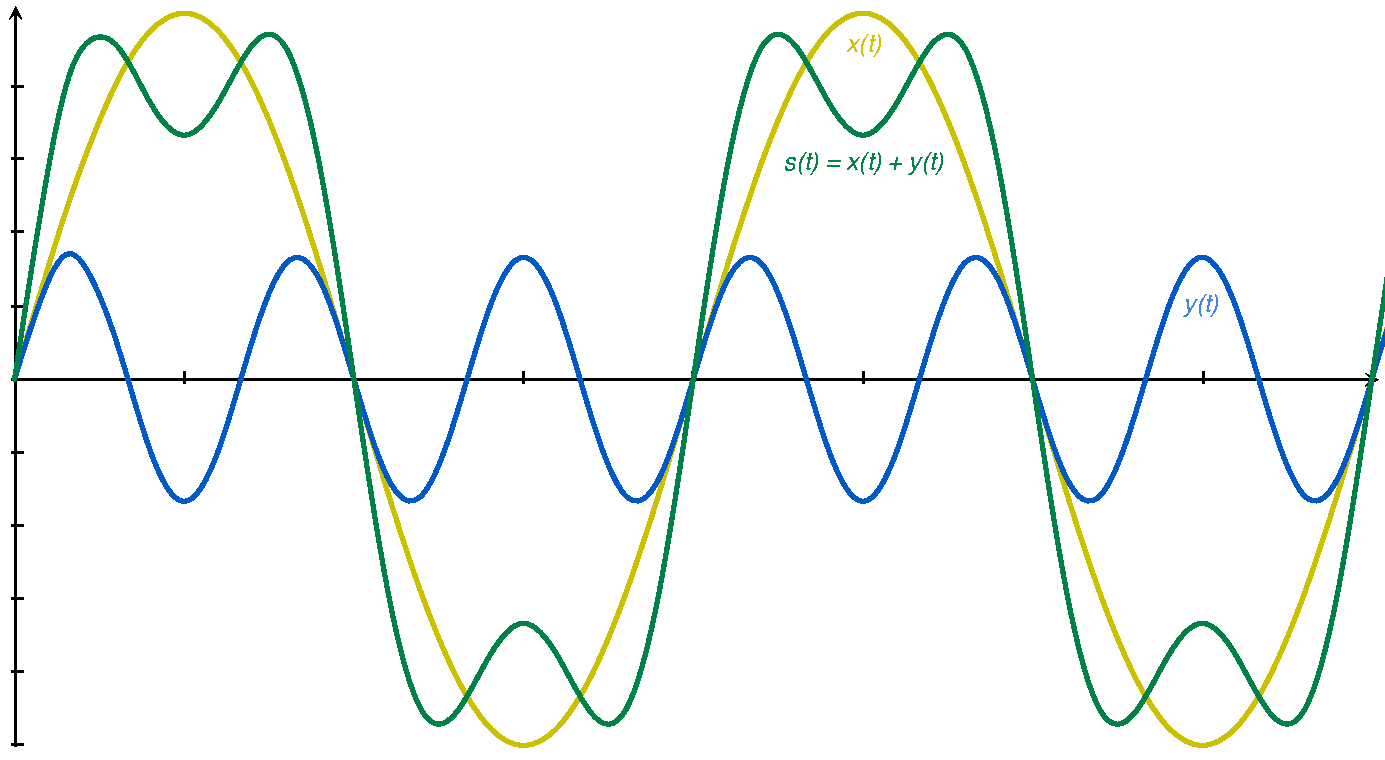
\includegraphics[scale=.5]{graphes/onde}
		\caption{Représentation graphique de l'onde $s(t)$}
	\end{figure}
\end{ex*}

\begin{rem*}
	De manière générale si l'on additionne à un signal périodique de période $T$ un autre signal périodique de période $\nicefrac{T}{n}$, le signal résultant est périodique de période $T$.
\end{rem*}

\section{Domaine temporel / Domaine fréquentiel} % (fold)

\subsection{La décomposition en séries de Fourier} % (fold)
Toute fonction périodique $g(t)$ de période $T$ peut se décomposer en une somme (éventuellement infinie) de fonctions sinus et cosinus.
\[
	g\left(t\right)=c_{0}+\sum_{n=1}^{\infty}a_{n}\cos\left(2\pi nf_{0}t\right)+\sum_{n=1}^{\infty}b_{n}\sin\left(2\pi nf_{0}t\right)
\]où
\begin{eqnarray*}
a_{n} & = & \frac{2}{T}\int_{\tau}^{\tau+T}g\left(t\right)\cos\left(2\pi nf_{0}t\right)\, dt\\
b_{n} & = & \frac{2}{T}\int_{\tau}^{\tau+T}g\left(t\right)\sin\left(2\pi nf_{0}t\right)\, dt\\
c_{0} & = & \frac{1}{T}\int_{\tau}^{\tau+T}g\left(t\right)\, dt\end{eqnarray*}

avec :\begin{itemize}
	\item $f_0$ la fréquence fondamentale,
	\item $a_n$ et $b_n$ sont les amplitudes sinus et cosinus de la $n^{\textrm{ième}}$ harmonique,
	\item $c_0$ est la composante continue du signal.
\end{itemize}
Une telle décomposition est appelée \textbf{Série de Fourier}. 

\begin{rem*}
	On a aussi :
	\[
		g(t)=c_0+\sum_{n=1}^{\infty}\sqrt{a_n^2+b_n^2}\cos(2\pi n f_0 t+\varphi_n)
	\]avec $\varphi_n=\arg(a_n+i b_n)$
\end{rem*}

\subsection{Spectre fréquentiel et largeur spectrale} % (fold)

Le spectre fréquentiel associé à une fonction périodique $g(t)$ est un \emph{spectre de raies}, chaque raie correspondant à la fréquence d'une harmonique de la décomposition en série de Fourier de $g(t)$. 

Il existe trois types de spectres fréquentiels :\begin{itemize}
	\item Le \textbf{spectre d'amplitude} pour lequel la hauteur de chaque raie est égale à $\sqrt{a_n^2+b_n^2}$ (leurs carrés sont proportionnels à la puissance transmise à la fréquence correspondante),
	\item Le \textbf{spectre de puissance} où chaque raie a une hauteur égale à $a_n^2+b_n^2$,
	\item Le \textbf{spectre de phase} où chaque raie possède une hauteur égale à $\arctan\left(\nicefrac{b_n}{a_n}\right)$.
\end{itemize}

\section{Bande passante} % (fold)

\subsection{Supports de transmission} % (fold)

Les supports physiques de transmission sont les éléments permettant de faire circuler les informations entre les équipements de transmission. 

On classe généralement ces supports en trois catégories, selon le type de grandeur physique qu'ils permettent de faire circuler, donc de leur constitution physique :\begin{itemize}
	\item Les supports \textbf{métalliques} permettent de faire circuler une grandeur électrique sur un câble généralement métallique ;
	\item Les supports \textbf{optiques} permettent d'acheminer des informations sous forme lumineuse ;
	\item Les supports \textbf{aériens} désignent l'air ou le vide; ils permettent la circulation d'ondes électromagnétiques diverses.
\end{itemize}

Selon le type de support physique, la grandeur physique a une vitesse de propagation plus ou moins rapide.

\begin{ex*}
	Le son se propage dans l'air à une vitesse de l'ordre de 300 m/s alors que la lumière a une célérité proche de 300 000 km/s
\end{ex*}

Un support de transmission ne peut transmettre que dans une bande de fréquence limitée.

\begin{def*}[Bande passante]
	On appelle \emph{bande passante} du support la bande de fréquences $\left[f_{1},\, f_{2}\right]$ ($f_1<f_2$), que le support laisse passer sans (trop de) déformation.
	
	La largeur de cette bande passante est généralement notée $B=f_2-f_1$.
\end{def*}

Or la transmission du signal complet requiert une largeur de bande infinie. La bande passante du support limite le débit qui peut être véhiculé sur le canal de transmission.

\begin{figure}[h!]
	\center
	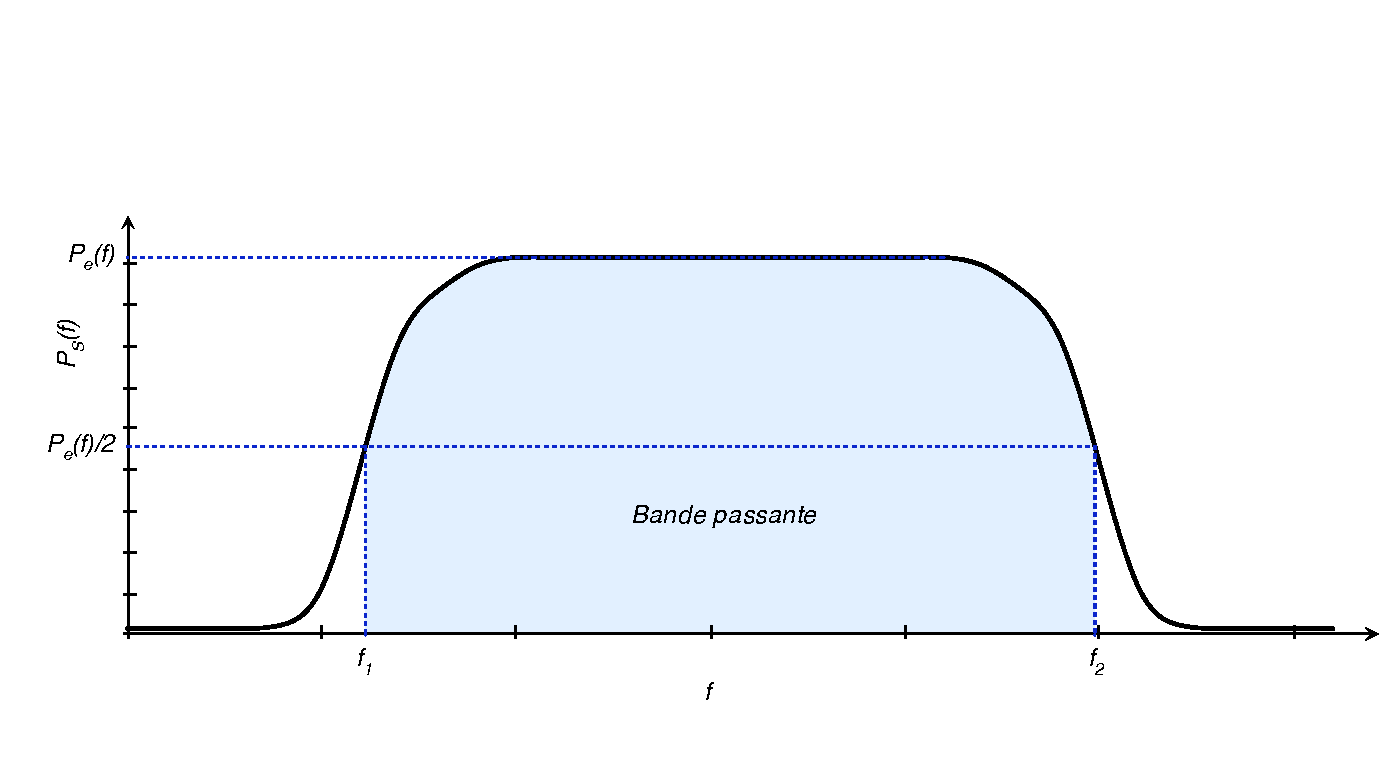
\includegraphics[scale=.5]{graphes/bandwidth}
	\caption{Représentation graphique de la bande passante $[f_1,\,f_2]$}
\end{figure}

\subsection{Perturbations du signal} % (fold)

On distingue généralement 3 types de perturbations du signal :\begin{itemize}
	\item \textbf{Affaiblissement de propagation} : perte de signal en énergie dissipée sur le support : Puissance reçue < Puissance émise. Plus le signal se propage, plus il est affaibli. 
	\item \textbf{Distorsion} : déformation subie par le signal -- certaines composantes fréquentielles sont plus atténuées que d'autres.
	\item \textbf{Bruit} : perturbation aléatoire qui se rajoute au signal sur tout support. On différencie :\begin{itemize}
		\item Les \emph{bruits blancs} : perturbation uniforme du signal -- ajoute au signal une petite amplitude de moyenne nulle ;
		\item Les \emph{bruits impulsifs} : petits pics de forte intensité et de faible durée ajoutés au signal.
	\end{itemize}
\end{itemize}

\begin{figure}[h!]
	\center
	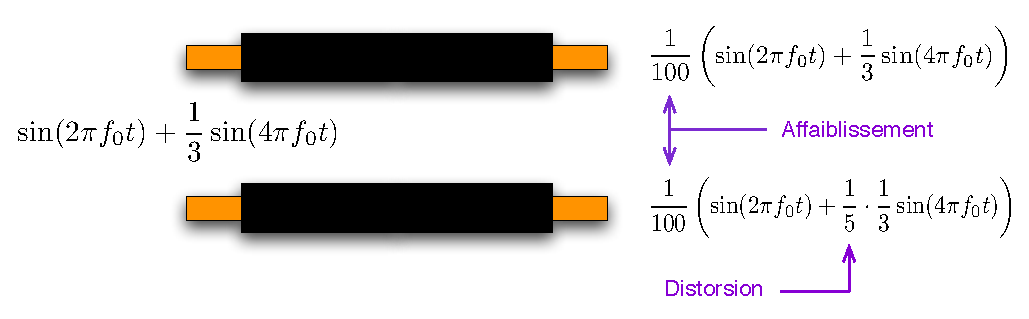
\includegraphics[scale=.75]{graphes/perturbations}
	\caption{Exemples de perturbations}
\end{figure}

\begin{def*}[Rapport Signal/Bruit]
 	Le rapport signal-à-bruit se calcule en faisant le quotient entre la puissance du signal $P_S$ et la puissance du bruit $P_N$. Il est exprimé en décibels (dB) :
\[
	\left(\frac{S}{N}\right)_{dB}=10\cdot\log_{10}\left(\frac{P_{S}}{P_{N}}\right)
\]
\end{def*}

\subsection{Bande passante et capacité} % (fold)

La loi de Shannon fournit le \textbf{débit binaire maximum} (\emph{capacité}) auquel on peut théoriquement transmettre \textbf{sans erreur} sur un canal à bande passante limitée sujet à du bruit.

\begin{loi*}[Shannon]
	Un canal de transmission bruité de largeur de bande $B$ a pour capacité :
	\[
		C=B\log_2\left(1+\frac{P_S}{P_N}\right) \qquad \textrm{(bit/s)}
	\] où $\nicefrac{P_S}{P_N}$ représente le rapport signal-à-bruit du canal.
\end{loi*}

\begin{figure}[h!]
	\center
	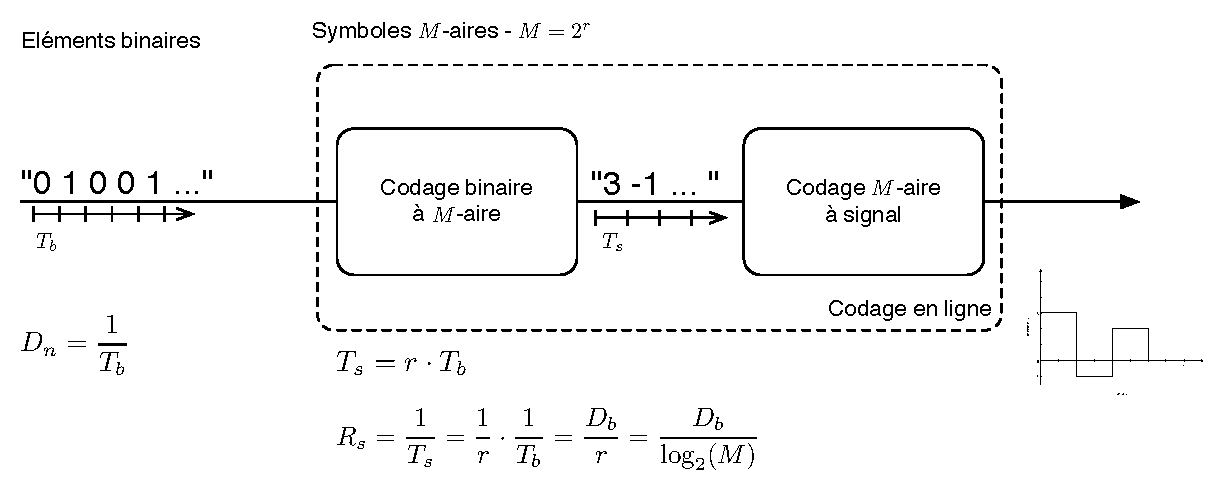
\includegraphics[scale=.75]{graphes/codage}
	\caption{Codage d'éléments binaires}
\end{figure}

\begin{loi*}[Nyquist]
	La rapidité de modulation $R_S$ d'un canal de largeur de bande $B$ doit vérifier :
	\[
		R_S \leqslant 2B \qquad \textrm{(symb/s)}
	\]
	
	Le débit binaire $D_b$ transmis sur un canal de largeur de bande $B$ doit donc vérifier :
	\[
		D_b \leqslant 2B\log_2 M \qquad \textrm{(bit/s)}
	\]
\end{loi*}

\chapter{Techniques de transmission et de protection contre les erreurs}

\section{Message, signal et modes de transmission} % (fold)

\begin{figure}[h!]
	\center
	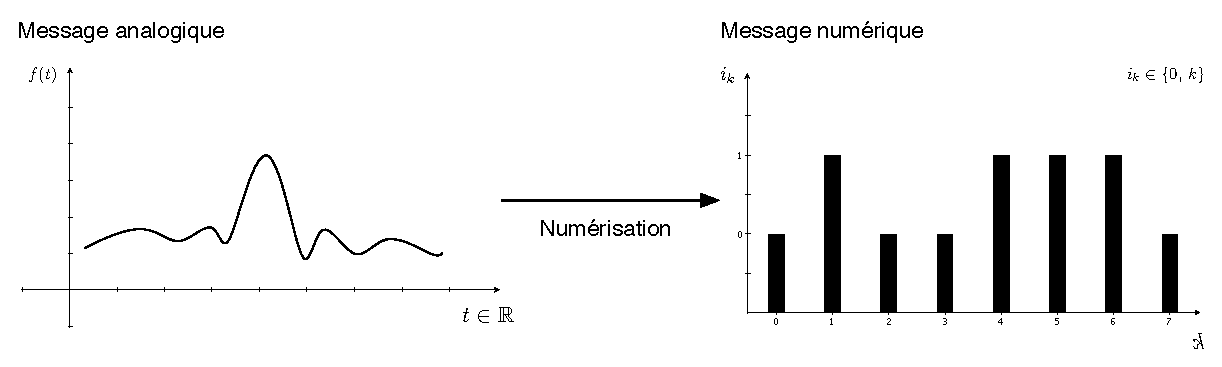
\includegraphics[scale=.75]{graphes/numerisation}
	\caption{Schéma de la numérisation}
\end{figure}

\begin{def*}[Message]
	Un message est constitué par les éléments d'information / données que l'usager soumet. 
	
	\begin{itemize}
		\item Message analogique : données se présentent sous la forme d'une fonction $f(t)$ continue.
		\item Message numérique : les données se présentent sous la forme d'i,e suite $\{i_k\}_{k\in\mathbb{N}}$ d'éléments d'information pouvant prendre une valeur parmi un ensemble fini de valeurs discrètes -- alphabet.
	\end{itemize}
\end{def*}

\begin{def*}[Signal]
	Un signal est la représentation physique du message à transmettre. C'est soit une onde électrique ou électromagnétique.
	
	\begin{itemize}
		\item Signal analogique : représente un message analogique.
		\item Signal numérique : signal résultant de la mise en forme d'un message numérique.
	\end{itemize}
\end{def*}

\begin{def*}[Transmission]
	La transmission est l'opération qui consiste à transporter le signal d'une machine vers une autre sur un support donné. On distingue la transmission analogique de la transmission numérique, suivant la nature du signal transmis.
	
	\begin{itemize}
		\item Transmission en bande de base : canal de type passe-bas (ie. de bande passante $[0,\,f_2]$). Il n'y a pas de modulation.
		\item Transmission sur fréquence porteuse : canal de type passe-bande (ie. de bande passante $[f_1,\,f_2]$). Le signal est alors modulé.
	\end{itemize}
\end{def*}

\begin{ex*}
	Un amplificateur est utilisé pour une transmission analogique. Il sert à amplifier (booster) le signal.
	
	Un répéteur est utilisé en transmission numérique. Il sert à :\begin{itemize}
		\item Décoder numériquement le signal (ie. retrouver les 0 et 1 transmis initialement).
		\item Reformer le signal sans bruit et amplifié.
	\end{itemize} 
\end{ex*}

\begin{figure}[h!]
	\center
	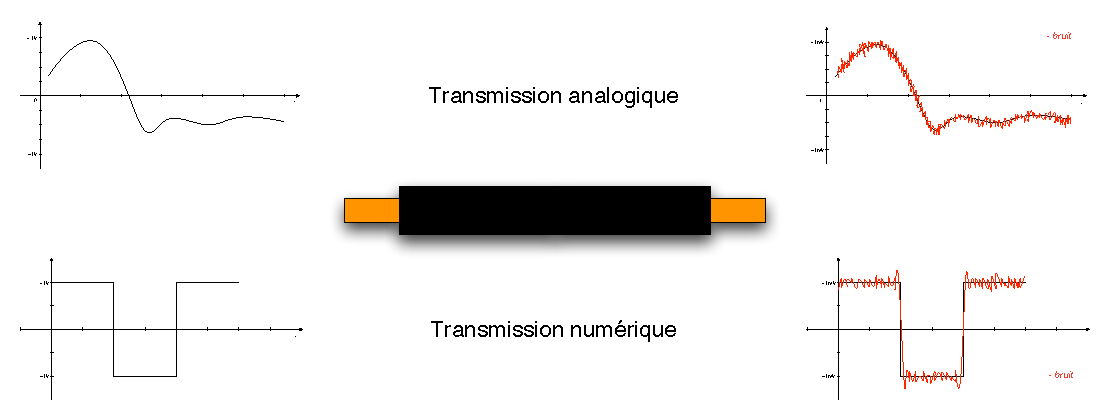
\includegraphics[scale=.75]{graphes/transmission}
	\caption{Transmission d'un signal analogique ou numérique}
\end{figure}

\section{La numérisation} % (fold)
\begin{def*}[Numérisation]
	La  numérisation est l'opération qui consiste à transformer un message analogique en un message numérique qui pourra ensuite être traité numériquement.
\end{def*}
Les trois étapes de la numérisation sont :\begin{itemize}
	\item \textbf{L'échantillonnage} : consiste à transformer un signal à temps continu en un signal à temps discret par un prélèvement périodique (de période $T_e$), à la fréquence d'échantillonnage, de la valeur du signal analogique ;
	\item \textbf{La quantification} représente un échantillon par une valeur numérique appartenant à une échelle de quantification. L'erreur de quantification est d'autant plus importante que le nombre de niveaux de quantification est faible et que le pas de quantification est grand ;
	\item \textbf{Le codage} consiste à remplacer la suite des valeurs quantifiées des échantillons par une suite binaire. S'il y a niveaux de quantification, chaque échantillon est codé sur $n$ bits.
\end{itemize}

\vspace{10pt}
Le théorème d'échantillonnage de Shannon exprime le nombre minimum d'échantillons par seconde nécessaire pour reconstituer un signal à partir de ses échantillons.
\begin{thm*}[Shannon]
	L'échantillonnage d'un signal de fréquence de spectre maximum $f_{\textrm{max}}$ est sans perte si :
	\[
		f_e >2\cdot f_{\textrm{max}}
	\]
	Pas d'échantillonnage (période):
	\[
		T_e = \frac{1}{f_e}
	\]
\end{thm*}

\begin{figure}[h!]
	\center
	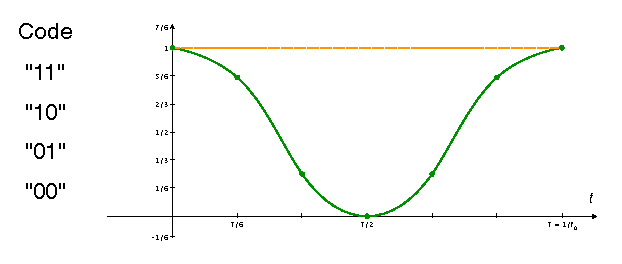
\includegraphics[scale=.7]{graphes/Quantification}
	\caption{Quantification d'un signal analogique}
\end{figure}

\section{Codage en ligne et transmission en bande de base} % (fold)

\begin{princ*}[Codage en ligne]
	Le codage en ligne consiste à associer une représentation physique au message numérique, avant d'effectuer une transmission numérique en bande de base (BdB) sur un support de longueur limitée. 
	
	Cette opération est parfois improprement appelée modulation en bande de base.
\end{princ*}

Le codage en ligne se décompose en 2 opérations :\begin{itemize}
	\item La première transforme la suite d'éléments binaires $\left\{d_k\right\}_{k\in\mathbb{N}}$ correspondant au message numérique à émettre en une suite de symboles. 
	
	C'est l'opération de codage binaire $M$-aire. 
	\item La seconde opération consiste à associer une forme d'onde à chaque symbole ainsi produit. 
	
	C'est l'opération de codage $M$-aire à signal.
\end{itemize}

\begin{def*}[Débit binaire]
	Débit binaire ($D_b$) : nombre maximum d'éléments binaires transmis par seconde.
	
	$T_b$ étant la durée de transmission d'un élément binaire, on a :
	\[
		D_b = \frac{1}{T_b} \qquad \textrm{bit/s}
	\]
\end{def*}

\begin{def*}[Rapidité de modulation]
	Rapidité de modulation ($R_s$): vitesse à laquelle les symboles se succèdent.
	
	$T$ étant la durée de transmission d'un symbole (et donc la durée d'un élément de signal), on a :
	\[
		R_s = \frac{1}{T_S}\qquad\textrm{symb/s (ou bauds)}
	\]
\end{def*}

\begin{def*}[Valence]
	Valence ($M$) : cardinal de l'alphabet des symboles.
	
	$r$ étant le nombre de bits codés par symbole, on a :
	\[
		M = 2^r \Leftrightarrow r= \log_2(M)\qquad\textrm{bits}
	\]
\end{def*}

\begin{rem*}
	La rapidité de modulation $R_s$ se relie au débit binaire $D_b$ par la relation suivante :
	\[
	 R_s = \frac{D_b}{r} = \frac{D_b}{\log_2(M)}\qquad\textrm{symb/s (ou bauds)}
	\]
	ou encore
	\[
		D_b = R_s.r = R_s.\log_2(M)\qquad\textrm{bit/s}
	\]
\end{rem*}

\section{Différents code en ligne} % (fold)

\subsection{Code NRZ (Non Return to Zero)} % (fold)

\begin{princ*}\hfill
	\begin{itemize}
		\item $d_k=0$, le signal vaut -V ;
		\item $d_k = 1$, le signal vaut V.
	\end{itemize}
\end{princ*}

Avantages :\begin{itemize}
	\item La détection de la présence ou non du signal ;
	\item $M = 2$ : bonne résistance aux bruits.
\end{itemize}
	          
Inconvénients :\begin{itemize}
	\item Spectre de puissance concentré autour de la fréquence nulle, coupée par de nombreux supports;
	\item Présence d'un courant continu lors d'une suite de 0 ou de 1, gênant la synchronisation entre émetteur et récepteur.
\end{itemize}

\subsection{Code Manchester (ou biphase)} % (fold)
\begin{princ*}\hfill
	\begin{itemize}
		\item $d_k=0$, le signal est un front \emph{montant} au milieu de l'intervalle $T_S$ ;
		\item $d_k = 1$, le signal est un front \emph{descendant} au milieu de l'intervalle $T_S$.
	\end{itemize}
\end{princ*}

Avantages :\begin{itemize}
	\item Spectre ne contenant pas la fréquence nulle ;
	\item Non passage par zéro, rendant possible par le récepteur la détection d'un signal ;
	\item Au moins une transition par intervalle.
\end{itemize}
	          
Inconvénient :\begin{itemize}
	\item Spectre de puissance concentré autour de la fréquence nulle, coupée par de nombreux supports.
\end{itemize}

\subsection{Code Manchester différentiel} % (fold)
\begin{princ*}\hfill
	\begin{itemize}
		\item $d_k=0$, le signal force une transition (front montant ou descendant) au début de l'intervalle $T_S$ et une autre au milieu de l'intervalle $T_S$;
		\item $d_k = 1$, le signal est un front \emph{descendant} au milieu de l'intervalle $T$.
	\end{itemize}
\end{princ*}

Avantages et inconvénients identiques au code Manchester.

Avantage par rapport au code Manchester :\begin{itemize}
	\item Une transition code ou non l'information, donc la polarité des fils n'a pas besoin d'être repérée.
\end{itemize}

\subsection{Code bipolaire simple} % (fold)
\begin{princ*}\hfill
	\begin{itemize}
		\item $d_k=0$, le signal vaut 0 ;
		\item $d_k = 1$, le signal vaut alternativement +V ou -V.
	\end{itemize}
\end{princ*}

Convention d'initialisation : amplitude de +V.

Avantage :\begin{itemize}
	\item Spectre limité.
\end{itemize}
	          
Inconvénients :\begin{itemize}
	\item Plus sensible au bruit que les codages à 2 niveaux ;
	\item Problèmes d'horloge avec les suites de 0.
\end{itemize}

\begin{figure}[h!]
	\center
	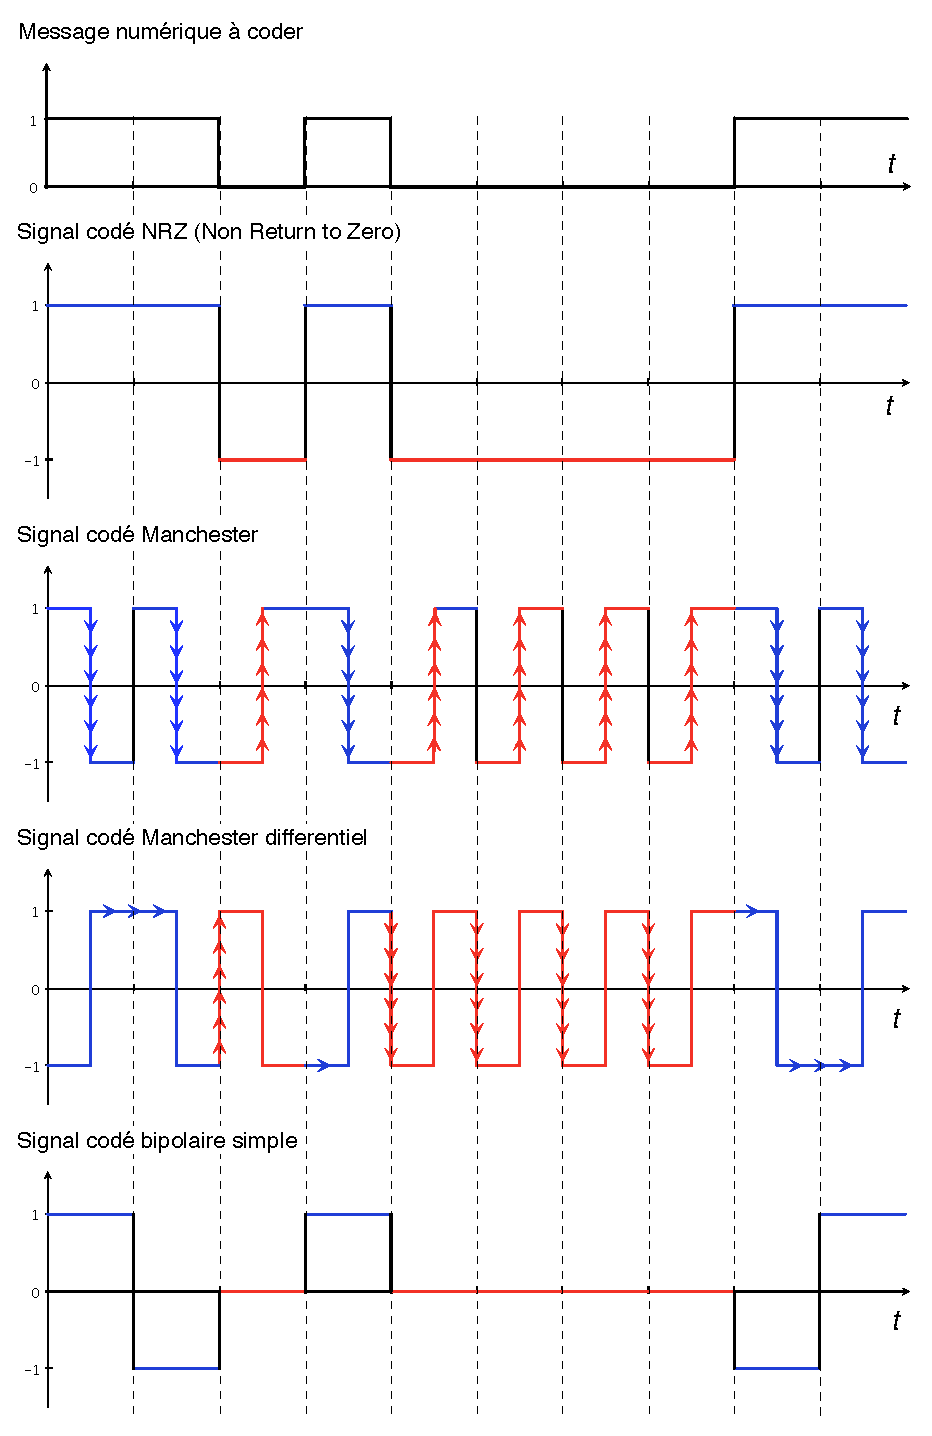
\includegraphics[scale=.9]{graphes/codages}
	\caption{Les différents types de codage d'un signal}
\end{figure}
\clearpage

\section{Modulation et transmission sur fréquences porteuses} % (fold)

	Lorsque le canal est de type passe-bande, comme dans le cas de la transmission hertzienne, il est indispensable de transposer le spectre du signal autour d'une fréquence porteuse située au centre de la bande passante du canal. On réalise ainsi une transmission sur fréquence porteuse.

\begin{princ*}[Modulation]
La technique de modulation permet de décaler le spectre du signal, naturellement situé autour de la fréquence nulle (signal en bande de base), autour d'une fréquence porteuse $f_0$. 

Elle est réalisée en modifiant (modulant) une des caractéristiques (amplitude, phase, fréquence instantanée) d'une porteuse sinusoïdale de fréquence $f_0$ en se servant du signal porteur de l'information à transmettre, appelé signal modulant. Lorsque le signal modulant est analogique on parle de modulation analogique.
\end{princ*}

Les modulations consistent à modifier l'amplitude, la phase ou la fréquence d'une porteuse sinusoïdale de fréquence $f_0$ en fonction de la valeur du symbole à transmettre sur chaque intervalle de durée $T_S$. Il existe donc trois grands types de modulation :\begin{itemize}
	\item \textbf{la modulation par déplacement d'amplitude} (MDA, ASK \emph{Amplitude Shift Keying}) qui associe à chaque symbole à coder une amplitude différente;
	\item \textbf{la modulation par déplacement de phase} (MDP, PSK \emph{Phase Shift Keying}) qui associe à chaque symbole à coder une phase différente;
	\item \textbf{la modulation par déplacement de fréquence} (MDF, FSK \emph{Frequency Shift Keying}) qui associe à chaque symbole à coder une fréquence différente.
\end{itemize}

Il existe aussi \textbf{la modulation par déplacement d'amplitude} (MDAP) et de phase ainsi que \textbf{la modulation d'amplitude en quadrature} (MAQ).

Le chiffre associé au sigle d'une modulation correspond au nombre total d'états possibles du signal modulé. Chaque état est associé à un symbole, le nombre d'états est donc égal à la valence $M$.

\begin{figure}[h!]
	\center
	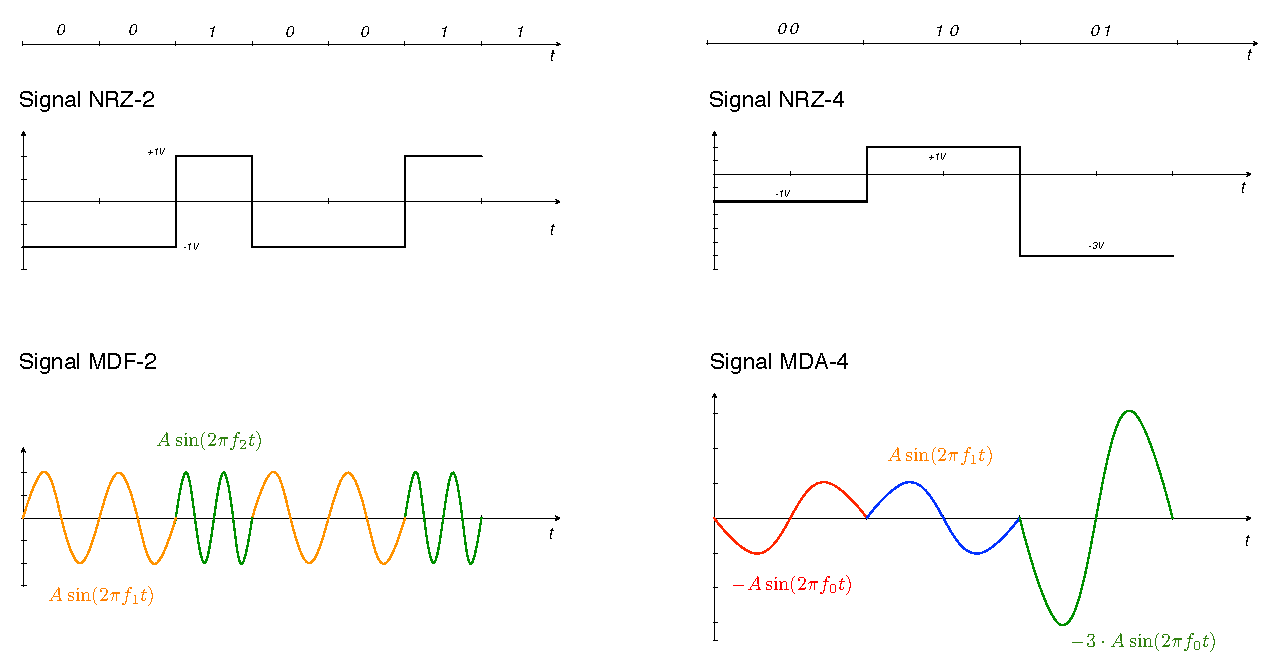
\includegraphics[scale=.7]{graphes/signals}
	\caption{Signal transmis sur fréquence porteuse}
\end{figure}

\section{Contrôle d'erreur} % (fold)

Lors de la transmission des données, un signal peut subir diverses déformations et être altéré par du bruit. A la réception, lors du décodage, une erreur d'estimation peut alors se produire: l'état du signal représentant le bit « 1 » est interprété comme s'il s'agissait d'un bit « 0 », et vice versa.

Plus le débit est élevé plus le risque que le bruit affecte plusieurs bits est grand.

\begin{def*}[Taux d'erreur binaire]
	Le taux d'erreur binaire (TEB) d'une transmission est défini comme le nombre moyen de bits transmis en erreur divisé par le nombre total de bits transmis.
\end{def*}

\begin{ex*}
	Quelques taux d'erreur binaire :\begin{itemize}
		\item $TEB_{\textrm{ligne téléphonique}}=10^{-5}$
		\item $TEB_{\textrm{câble coaxial}}=10^{-7}\textrm{ à }10^{-8}$
		\item $TEB_{\textrm{fibre optique}}=10^{-10}\textrm{ à }10^{-12}$
	\end{itemize}
\end{ex*}


Les techniques employées, pour effectuer un contrôle d'erreurs, reposent sur l'utilisation de \emph{codes détecteurs} ou de \emph{codes correcteurs} d'erreurs qui enrichissent la suite de bits à envoyer, en lui ajoutant de la redondance. Le récepteur se sert de cette information ajoutée pour déterminer si une erreur s'est produite et éventuellement pour la corriger.

\begin{def*}[Mot]
	Pour $m$ \emph{bits de données}, on ajoutera $r$ \emph{bits de redondance} pour permettre la détection et éventuellement la correction d'erreurs. On transmettra au total $n = m + r$ bits.
	\begin{itemize}
		\item Mot \textbf{légal} : les bits de contrôle correspondent aux bits de données ;
		\item Mot \textbf{illégal} sinon. La réception d'un mot de code illégal permet de détecter la présence d'une erreur.
	\end{itemize}
\end{def*}

On a alors :\begin{itemize}
	\item Nombre de mots de code possibles : $2^n$;
	\item Nombre de mots de code légaux possibles : $2^m$;
	\item Nombre de mots de code illégaux possibles : $2^n - 2^m$.
	
\end{itemize}

\subsection{Codes de détection d'erreurs basés sur la parité} % (fold)

Prenons un mot de 7 bits, on lui ajoute un bit de contrôle de valeur telle que le nombre total de bits à 1 du code du caractère est pair. C'est ce qu'on appelle un bit de parité ou \textbf{VRC (Vertical Redundancy Checking)}.\\
Pouvoir de détection d'erreur : 1 par mot.
\begin{ex*}
	Soit le mot 
	\[
		\begin{array}{ccccccc}
		\mathtt{1} & \mathtt{0} & \mathtt{0} & \mathtt{1} & \mathtt{1} & \mathtt{1} & \mathtt{1}\end{array}
	\]
	
	Le mot obtenu par VRC est alors : 
	\[
		\begin{array}{cccccccc}
		\mathtt{1} & \mathtt{0} & \mathtt{0} & \mathtt{1} & \mathtt{1} & \mathtt{1} & \mathtt{1} & \mathtt{{\color{red}1}}\end{array}
	\]
\end{ex*}

On utilise aussi la parité bidimensionnelle ou \textbf{LRC (Longitudinal Redundancy Checking)}.\\
Pouvoir de détection d'erreur : 3\\
Pouvoir de correction d'erreur : 1

\begin{ex*}
	Soit le code 
	\[
		\begin{array}{ccccccc}
		\mathtt{1} & \mathtt{0} & \mathtt{0} & \mathtt{1} & \mathtt{1} & \mathtt{1} & \mathtt{1}\\
		\mathtt{1} & \mathtt{0} & \mathtt{1} & \mathtt{0} & \mathtt{0} & \mathtt{1} & \mathtt{1}\\
		\mathtt{1} & \mathtt{0} & \mathtt{0} & \mathtt{0} & \mathtt{0} & \mathtt{1} & \mathtt{1}
		\end{array}
	\]
	
	Le code obtenu par LRC est alors :
	\[
		\begin{array}{cccccccc}
		\mathtt{1} & \mathtt{0} & \mathtt{0} & \mathtt{1} & \mathtt{1} & \mathtt{1} & \mathtt{1} & {\color{red}\mathtt{1}}\\
		\mathtt{1} & \mathtt{0} & \mathtt{1} & \mathtt{0} & \mathtt{0} & \mathtt{1} & \mathtt{1} & {\color{red}\mathtt{0}}\\
		\mathtt{1} & \mathtt{0} & \mathtt{0} & \mathtt{0} & \mathtt{0} & \mathtt{1} & \mathtt{1} & {\color{red}\mathtt{1}}\\
		{\color{green}\mathtt{1}} & {\color{green}\mathtt{0}} & {\color{green}\mathtt{1}} & {\color{green}\mathtt{1}} & {\color{green}\mathtt{1}} & {\color{green}\mathtt{1}} & {\color{green}\mathtt{1}} & {\color{green}\mathtt{0}}\end{array}
	\]
\end{ex*}

\subsection{Codes de détection d'erreurs polynomiaux}

A un code polynomial $C$ est associé un polynôme générateur (par ex: $g(x) = x^8 + 1$).
Le codage est la calcul du mot de code :\begin{itemize}
	\item On constitue $M(x)$ le polynôme associé à la suite binaire à transmettre ;
	\item On multiplie $M(x)$ par $x^r$, où $r$ est le degré du polynôme générateur $g(x)$;
	\item On calcule $R(x)$, le reste de la division du polynôme $M(x)* x^r$ par $g(x)$;
	\item On calcule le mot de code  $M(x)* x^r  - R(x)$ et on le transmet.
\end{itemize}

\vspace{10pt}
Le décodage est la vérification du mot de code reçu :\begin{itemize}
	\item On constitue $M'(x)$ le polynôme associé à la suite binaire reçue;
	\item On calcule $R'(x)$, le reste de la division du polynôme de $M'(x)$ par $R'(x)$:\begin{itemize}
		\item Si $R'(x) = 0$; il n'y a pas d'erreur;
		\item Sinon il y a une erreur, on demande alors la retransmission du message.
	\end{itemize}
\end{itemize}

\chapter{Liaison de données} % (fold)

\section{Introduction} % (fold)

Lorsque l'on souhaite faire communiquer deux équipements informatiques \textbf{ETTD} (Equipement Terminal de Traitement de Données), on commence par mettre en oeuvre un circuit de données, constitué d'un support de transmission et de deux \textbf{ETCD} (Equipement de Terminaison de Circuit de Données), qui permet d'émettre et/ou de recevoir des bits en série sur le support physique.

Mais avec :\begin{itemize}
	\item Un certain débit;
	\item Un certain délai (temps de transmission et de propagation);
	\item Un certain taux d'erreurs,
\end{itemize}
le circuit de données n'est pas suffisant pour assurer un transport et une interprétation corrects de l'information entre les deux ETTD (aucun moyen de réagir à des anomalies de transmission). 

Il est donc nécessaire d'ajouter une interface logique entre la partie de traitement de l'information et la partie de transmission de l'information. Cette interface, appelée procédure de commande ou protocole de communication, est chargée de fiabiliser le transfert de l'information entre deux ETTD.

La liaison de données est donc constituée du circuit de données et du protocole de communication.

\begin{figure}[h!]
	\center
	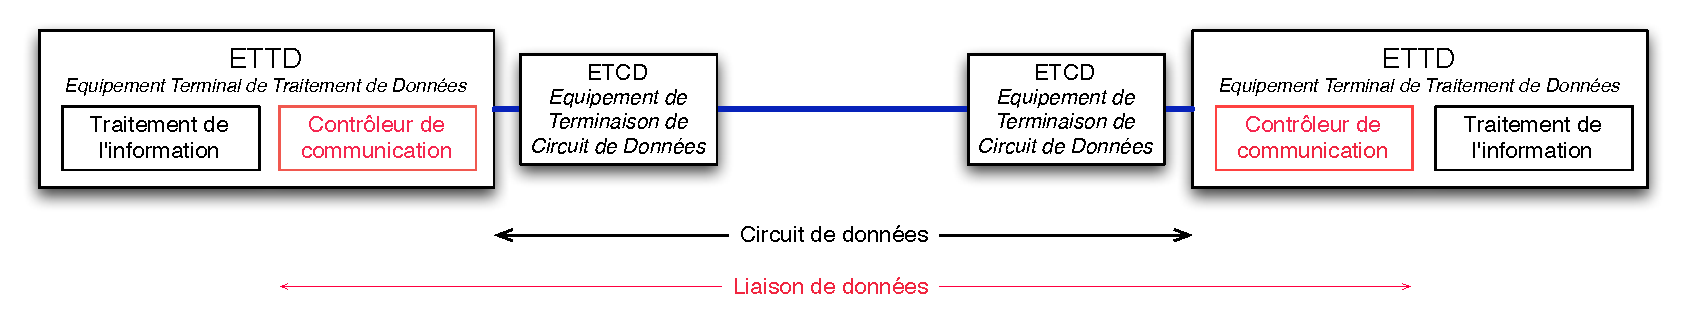
\includegraphics[scale=.5]{graphes/ETTD}
	\caption{Liaison de données}
\end{figure}

\begin{def*}[Fialbilité]
	Pas d'erreur, pas de perte, pas de déséquencement, pas de duplication.
\end{def*}

\section{Caractéristiques d'une liaison de données} % (fold)

\begin{description}
	\item[Configuration] \textbf{point-à-point} ou \textbf{multipoint}.
	\item[Mode d'exploitation] \textbf{unidirectionnel}, \textbf{bidirectionnel} à l'\textbf{alternat} ou \textbf{bidirectionnel simultané}.
	\item[Mode de gestion] L'échange d'information entre deux stations sur une liaison doit être réglé de façon précise afin d'éviter que des stations n'émettent simultanément en se brouillant réciproquement, ou de permettre une configuration de la réception des données transmises. Deux approches sont possibles :\begin{itemize}
		\item Approche \textbf{centralisée} (ou hiérarchique) : une station primaire joue un rôle particulier dans le protocole pour assurer que la communication entre plusieurs stations secondaires se passe sans problèmes;
		\item Approche \textbf{symétrique} : toutes les stations ont les « mêmes droits » et les « mêmes devoirs », donc un rôle symétrique vis-à-vis du protocole de communication
	\end{itemize}  
\end{description}

\section{Conception d'un protocole de liaison de données} % (fold)

Une liaison de données est constituée d'un canal physique capable de transmettre des bits en série, sur lequel sont raccordés un certain nombre (2 ou plus) de stations qui doivent pouvoir échanger de l'information. Cette information est structurée en trames.

En plus des trames d'information contenant les données, il faut gérer la liaison, pouvoir échanger des trames de contrôle (ou de commande ou de supervision).

\begin{def*}[Protocole de liaison de données]
	Un protocole de liaison de données (ou procédure de contrôle) est un ensemble de règles permettant de gérer la liaison :\begin{itemize}
		\item Règle de codage des informations de contrôle;
		\item Règle de structuration (séparation de l'information proprement dite de l'information de contrôle);
		\item Règle d'échange (pour préciser les séquences valides d'échanges de trames).
	\end{itemize}
	
	Ce protocole met en oeuvre un certain nombre de mécanismes de communication sur la liaison pour atteindre l'objectif de fiabilité.
\end{def*}

\section{Quelques mécanismes et leurs principes} % (fold)

\subsection*{La délimitation de trames} % (fold)

\begin{figure}[h!]
	\center
	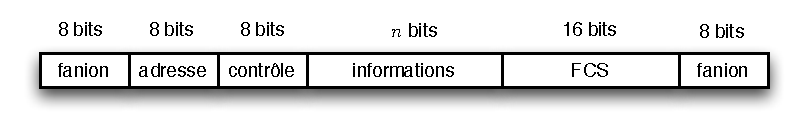
\includegraphics[scale=.7]{graphes/trame}
	\caption{Une trame HDLC}
\end{figure}

On va choisir une combinaison particulière (par exemple « 01111110 ») comme délimiteur ou \textbf{fanion} (flag).

\begin{description}
	\item[Problème] Les données utilisateurs sont quelconques et peuvent en particulier contenir la combinaison retenue pour le fanion.
	\item[Solution] En émission, un « 0 » (bit de bourrage) est inséré dés que cinq « 1 » binaire consécutifs apparaissent en dehors des champs fanions. Ces « 0 » sont retirés à la réception.
\end{description}

\subsection*{L'établissement et la libération de la liaison de données} % (fold)

\begin{def*}[Etablissement de la liaison]
	Une fois les stations raccordées physiquement au canal de transmission elles doivent échanger de l'information de contrôle avant de pouvoir échanger les données proprement dites. 
	
	Cette information de contrôle permet en particulier aux stations de se reconnaître mutuellement et d s'assurer qu'elles sont prêtes à communiquer. 
\end{def*}

A l'issue de cette phase, il y a la phase de \textbf{transfert de données}.

\begin{def*}[Libération de la liaison]
	Lorsque les stations n'ont plus de données à échanger, elles échangent à nouveau des informations de contrôle pour terminer le transfert de l'information.
\end{def*}

\begin{figure}[h!]
	\center
	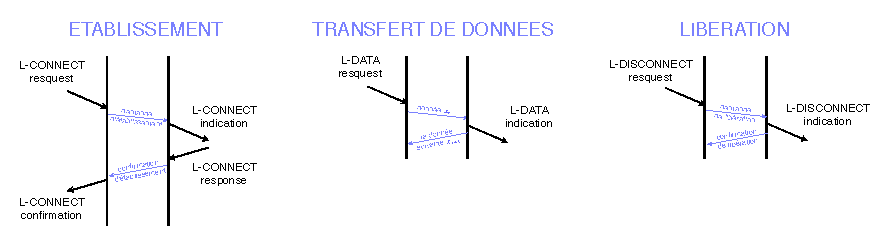
\includegraphics[scale=1.2]{graphes/transfert_data}
	\caption{Transfert d'une trame}
\end{figure}

\subsection*{Le contrôle de flux} % (fold)
Il s'agit d'asservir l'émetteur de façon à ce qu'il émette à un taux inférieur aux taux d'absorption du récepteur.

\begin{princ*}[\emph{Send-and-Wait}]
	Chaque fois qu'il a fini d'envoyer une trame, l'émetteur attend l'autorisation explicite du récepteur pour envoyer la trame suivante.
\end{princ*} 

\subsection*{La détection d'erreur} % (fold)

\begin{description}
	\item[Problème] Le circuit de données n'étant pas parfait, il peut se produire des erreurs de transmission.
	\item[Solution] Inclure dans la trame un champ de contrôle calculer selon une technique \textbf{CRC} (Cycling Redundancy Check) par exemple, qui permettra au récepteur de détecter les erreurs dans la trame et donc de \textbf{rejeter} la trame erronée.
\end{description}

\begin{figure}[h!]
	\center
	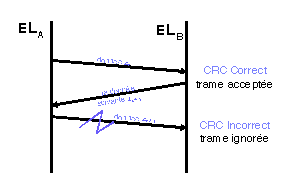
\includegraphics[scale=1.2]{graphes/erreur_transmission}
	\caption{Détection d'erreur}
\end{figure}

\subsection*{Les acquittements} % (fold)
Si la trame est en erreur, le récepteur doit demander une retransmission de la trame. Si elle est correcte le récepteur doit autoriser l'émetteur à passer à la trame suivante.

\begin{description}
	\item[NAK] Acquittement négatif pour signaler une erreur de transmission et demander une retransmission.
	\item[ACK] Acquittement positif, demande la transmission de la trame suivante.
\end{description}

\begin{figure}[h!]
	\center
	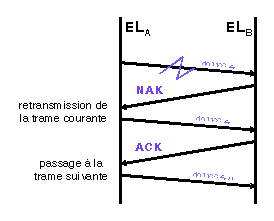
\includegraphics[scale=1.2]{graphes/acquittement}
	\caption{Acquittement}
\end{figure}

\subsection*{Le temporisateur de retransmission} % (fold)
Pour éviter que l'émetteur ne reste indéfiniment en attente d'une réponse hypothétique (interblocage) du récepteur, on utilise un mécanisme de temporisation.

\begin{wrapfigure}{l}{0.60\textwidth}
	\vspace{-15pt}
	\begin{center}
		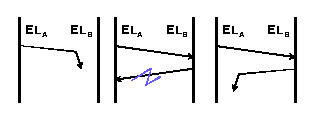
\includegraphics[width=0.40\textwidth]{graphes/temporisation1}
		\vspace{-15pt}
		\caption{Problèmes de transmission de données}
	\end{center}
	
\end{wrapfigure}

\begin{wrapfigure}{r}{0.50\textwidth}
	\vspace{-60pt}
	\begin{center}
		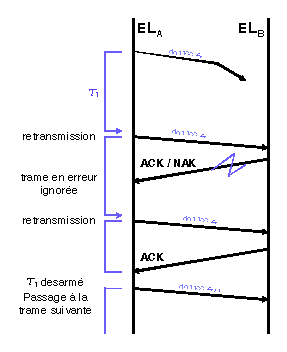
\includegraphics[width=0.38\textwidth]{graphes/temporisation2}
		\vspace{-15pt}
		\caption{Temporisateur de retransmission}
	\end{center}
	\vspace{-40pt}
\end{wrapfigure}

A l'émission d'une trame, l'émetteur arme un temporisateur dont la durée $T$ est supérieure au délai aller-retour légèrement surestimé d'une trame (\textbf{Round-Trip Time}).

Si le temporisateur arrive à échéance avant qu'un acquittement ne soit reçu, la trame est retransmise. Dans le cas contraire, il est désarmé.

Pour éviter un nombre infini de retransmission suite à un accident grave du circuit de données, le nombre de transmission pour une même trame est limité à $N$. Au bout de $N$ essais infructueux, la liaison est considérée hors service.

\begin{rem*}
	La retransmission des trames suppose une rétention des trames (on garde une copie des trames non encore transmises).
\end{rem*}

\subsection*{La numérotation des trames} % (fold)

\begin{figure}[h!]
	\center
	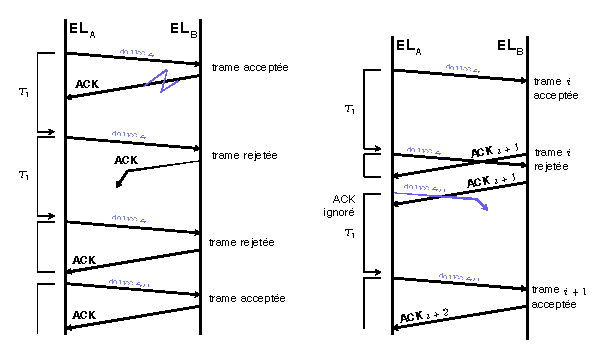
\includegraphics[scale=1.2]{graphes/numerotation}
	\caption{Numérotation de trames}
\end{figure}

\begin{description}
	\item[Solution] introduire dans la trame de données un champ véhiculant son numéro de séquence $N(S)$.
\end{description}

\begin{rem*}
	pour une procédure \emph{Send-and-Wait} une numérotation modulo 2 sur un seul bit suffira puisqu'il ne peut jamais avoir plus de deux trames non encore acquittées.
	
	Il y a aussi une numérotation des acquittements (au moins les 	positifs). On utilise un numéro $N(R)$ qui correspond au numéro de la prochaine trame attendue par le récepteur.
\end{rem*}

\subsection*{Le temporisateur de détection d'inactivité} % (fold)

\begin{description}
	\item[Problème] Hormis les erreurs de retransmission et les pertes de trame, il peut y avoir des accidents graves comme la rupture du circuit de données.
	\item[Solution] Utiliser un temporisateur I qui sera réarmé lors de toute trace d'activité du distant.
\end{description}

\begin{figure}[h!]
	\center
	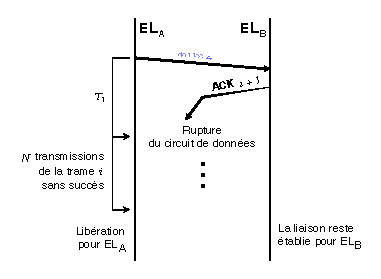
\includegraphics[scale=1.2]{graphes/inactivite}
	\caption{Inactivité du canal de transmission}
\end{figure}

\subsection*{La fenêtre d'anticipation} % (fold)

Lorsque le circuit de données présente un temps de propagation important (ex: liaison satellite) une procédure type \emph{Send-and-Wait} ne permet pas d'utiliser d'une manière efficace la bande passante.

Une solution consiste à permettre à l'émetteur d'envoyer consécutivement $W$ trames avant de se bloquer.

\begin{princ*}[Fenêtre coulissante]
	 L'émetteur est autorisé à envoyer les trames de numéro de séquence $N(S)$ compris entre le numéro r de la prochaine trame attendue (communiqué par le récepteur dans les champ $N(R)$) et $r + W - 1$.
	\[
		r = N(R) \leqslant N(S) \leqslant r+W-1
	\]
\end{princ*}

\begin{rem*}
	L'utilisation d'une fenêtre d'anticipation peut nécessiter la mise en oeuvre d'un mécanisme de régulation supplémentaire de type « tout ou rien ».
\end{rem*}

\begin{description}
	\item[Solution] Une trame de contrôle particulière est utilisée pour indiquer que le récepteur est momentanément dans l'incapacité de continuer à recevoir (ex: trame \textbf{RNR} dans HDLC -- \emph{not ready to receive}).
\end{description}

\begin{princ*}[Mécanisme de rejet]
	L'utilisation d'une fenêtre implique que parmi les trames non encore acquittées certaines peuvent ne pas être reçues correctement. Le récepteur doit alors rejeter ces trames.
\end{princ*}

\begin{description}
	\item[Solutions] \hfill \begin{itemize}
		\item Le rejet sélectif (\textbf{SREJ}) seule la trame en erreur doit être retransmise;
		\item Le rejet global (\textbf{REJ}) la trame erronée ainsi que toutes les trames qui la suivent sont rejetées et doivent être retransmises.
	\end{itemize}
\end{description}

\section{Protocole HDLC} % (fold)

\subsection{Généralités} % (fold)

\begin{description}
	\item [HDLC] \emph{High-level Data Link Control}
	\item[Norme ISO] \hfill\begin{itemize}
		\item IS 3309-2 : structure de trames;
		\item IS 4335 : éléments de procédures.
	\end{itemize}
	\item[Configuration] \hfill\begin{itemize}
		\item Point-à-point;
		\item Multipoint.
	\end{itemize}
	\item[Exploitation] \hfill\begin{itemize}
		\item Bidirectionnel à l'alternat;
		\item Bidirectionnel simultané.
	\end{itemize}
	\item[Procédure orientée bit] Utilisation de trames de longueur quelconque et constituée de plusieurs champs (données ; information de contrôle ; début/fin : fanions).
	\item[Fonctionnement] Mode connecté :\begin{description}
		\item [Mode NRM (\emph{Normal Response Mode})] \hfill\begin{itemize}
			\item Liaison point-à-point ou multipoint;
			\item Gestion hiérarchique (une station primaire, des stations secondaires);
			\item Exploitation par élection.
		\end{itemize}
		\item [Mode ARM (\emph{Asynchronus Response Mode})] \hfill\begin{itemize}
			\item Liaison point-à-point ou multipoint;
			\item Gestion hiérarchique (une station primaire, des stations secondaires);
			\item Exploitation par compétition.
		\end{itemize}
		\item [Mode ABM (\emph{Asynchronous Balanced Mode})] \hfill\begin{itemize}
			\item liaison point-à-point;
			\item gestion symétrique (stations identiques).
		\end{itemize}
	\end{description}
	\begin{rem*}
		Aujourd'hui, seul le mode ABM est utilisé. Il s'applique sur une liaison point-à-point. Liaison symétrique : chaque station dispose des capacités d'initialisation, de supervision et de reprise (peut envoyer trames de commande ou de réponse).
	\end{rem*}
	\item[Fenêtre d'anticipation] \hfill\begin{itemize}
		\item 7 : mode normal;
		\item 127 : mode étendu.
	\end{itemize}
\end{description}

\clearpage

\subsection{Structure de la trame} % (fold)

\begin{figure}[h!]
	\center
	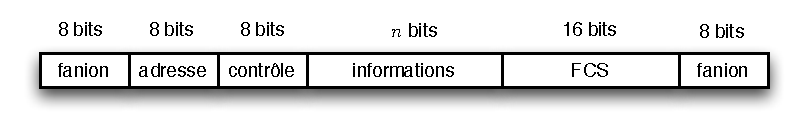
\includegraphics[scale=.8]{graphes/trame}
	\caption{Une trame HDLC}
\end{figure}


\begin{description}
	\item [Fanion (\emph{flag})] \lstinline!01111110! \begin{itemize}
		\item Délimitation de trame : toute trame commence et finit par un fanion;
		\item Synchronisation de trame : toutes les stations rattachées à la liaison doivent rechercher en permanence cette séquence;
		\item Un même fanion peut servir de fermeture pour une trame et de fanion d'ouverture pour la trame suivant.
		\item Mécanisme de transparence au fanion par bits de bourrage : en émission un \lstinline!0! est inséré dès que cinq \lstinline!1! consécutifs apparaissent en dehors des champs fanion. Ces \lstinline!0! sont enlevés en réception.
	\end{itemize}
	\begin{rem*}
		Si sept \lstinline!1! apparaissent n'import où dans une trame, elle est déclarée comme erreur.
	\end{rem*}
	\item[Champ adresse] Permet d'identifier la trame comme étant une commande ou une réponse :\begin{itemize}
		\item Trame de commande : l'adresse est celle du destinataire de la trame.
		\item Trame de réponse : l'adresse est celle de l'émetteur de la trame.
	\end{itemize}
	\item[Champ de contrôle] Indique le type de la trame :\begin{description}
		\item [Trame I (\emph{Information})] Mécanisme de \emph{piggbacking} -- acquittement dans les données.
		
		\begin{figure}[h!]
			\vspace{-15pt}
			\center
			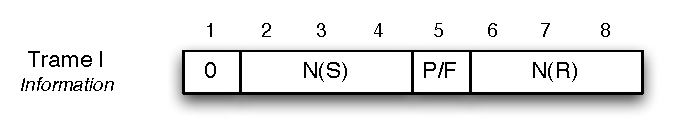
\includegraphics[scale=.75]{graphes/trameI}
			\vspace{-20pt}
		\end{figure}
		\item [Trame S (\emph{Supervision})] Assurer les fonctions de supervision de base de la liaison.
		
		\begin{figure}[h!]
			\vspace{-15pt}
			\center
			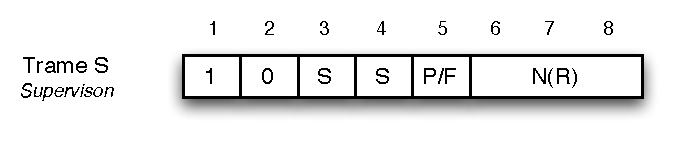
\includegraphics[scale=.75]{graphes/trameS}
			\vspace{-20pt}
		\end{figure}
	\begin{tabularx}{\linewidth}{>{\setlength\hsize{0.6\hsize}}X>{\setlength\hsize{1.75\hsize}}X>{\setlength\hsize{0.65\hsize}}X}
		RR & \emph{Ready to Recieve} $N\left(R\right)$ & \lstinline!1 0 0 0 P/F N(R)!\tabularnewline
		REJ & \emph{Reject} $N\left(R\right)$ & \lstinline!1 0 0 1 P/F N(R)!\tabularnewline
		SREJ & \emph{Selective Reject} $N\left(R\right)$ & \lstinline!1 0 1 0 P/F N(R)!\tabularnewline
		RNR & \emph{Not Ready to Recieve} & \lstinline!1 0 1 1 P/F N(R)!\tabularnewline
		\end{tabularx}
		\item [Trame U (\emph{Unnumbered})] Ne comporte pas de numéro -- établissement et libération de la liaison.
		
		\begin{figure}[h!]
			\vspace{-15pt}
			\center
			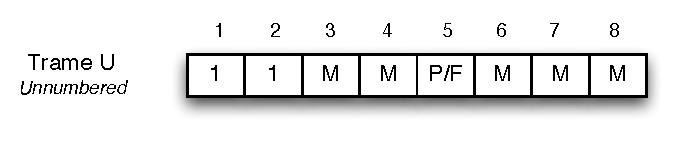
\includegraphics[scale=.75]{graphes/trameU}
			\vspace{-20pt}
		\end{figure}
		\begin{tabularx}{\linewidth}{>{\setlength\hsize{0.6\hsize}}X>{\setlength\hsize{1.75\hsize}}X>{\setlength\hsize{0.65\hsize}}X}
		SNRM & \emph{Set NRM} & \lstinline!1 1 0 0 P 0 0 1!\tabularnewline
		SARM & \emph{Set ARM} & \lstinline!1 1 1 1 P 0 0 0!\tabularnewline
		SABM & \emph{Set ABM} & \lstinline!1 1 1 1 P 1 0 0!\tabularnewline
		SNRME & \emph{Set NRM Extended} & \lstinline!1 1 1 1 P 0 1 1!\tabularnewline
		SARME & \emph{Set ARM Extended} & \lstinline!1 1 1 1 P 0 1 0!\tabularnewline
		SABME & \emph{Set ABM Extended} & \lstinline!1 1 1 1 P 0 1 1!\tabularnewline
		UA & \emph{Unnumbered Acknowledge} & \lstinline!1 1 0 0 F 1 1 0!\tabularnewline
		DISC & \emph{Disconnect} & \lstinline!1 1 0 0 F 0 0 1!\tabularnewline
		CMDR / FRMR & \emph{Command} (ARM, NRN) / \emph{Frame} (ABM) \emph{Reject} & \lstinline!1 1 1 0 P 0 1 0!\tabularnewline
		DM & \emph{Disconnect Mode} & \lstinline!1 1 1 1 F 0 0 0!\tabularnewline
		\end{tabularx}
	\item [Description des champs] \hfill\begin{itemize}
			\item Le champ $N(S)$ indique le numéro de séquence de la trame;
			\item Le champ $N(R)$ indique le numéro de la prochaine trame attendue.
			\item Le champ $P/F$ :\begin{itemize}
				\item $P$ (\emph{Poll}) : demande de réponse immédiate pour les commandes;
				\item $F$ (\emph{Final}) : réponse au bit $P$ ou trame finale (en NRM).
			\end{itemize}
			\item Jusqu'à 4 trames S différentes;
			\item Jusqu'à 32 trames U différentes.
	\end{itemize}
	\end{description}
	\item[Champ information] \hfill\begin{itemize}
		\item Données de l'utilisateur;
		\item Toute trame de longueur inférieure à 6 octets est non valide.
	\end{itemize}
	\item[FCS (\emph{Frame Check Sequence})] Calculé sur les champs d'adresse, de commande et d'information à partir du code polynomial V.41 : $x^{16}+x^{12}+x^5+1$
\end{description}

\subsection{Situations d'erreur et anomalies de fonctionnement} % (fold)

\begin{description}
	\item [Station temporairement saturée] \hfill\begin{itemize}
		\item Indication d'un état d'occupation : émission d'une trame RNR avec un $N(R)$ indiquant le numéro de séquence de la première trame non acceptée.
		\item Indication du retour à l'état normal : émission d'une trame RR (ou d'une trame I) avec $N(R)$ indiquant le numéro de séquence de la prochaine trame attendue.
	\end{itemize}
	\item[Erreurs de transmission] \hfill \begin{itemize}
		\item Rejet des trames dont le FCS indique la présence d'erreurs de transmission;
		\item \textbf{Tout se passe comme si la station n'avait rien reçu}.
	\end{itemize}
	\item[Erreurs de numéro de séquence] Le $N(S)$ ne correspond pas au numéro de la prochaine trame attendue : émission d'une trame de rejet : \begin{itemize}
		\item REJ : mécanisme de rejet non sélectif : toutes les trames qui suivent la trame erronée sont rejetées ;
		\item SREJ : mécanisme de rejet sélectif : seule la trame erronée est rejetée ; les autres sont mémorisées.
	\end{itemize}
\end{description}

\chapter{Commutation et multiplexage} % (fold)

\section{Commutation} % (fold)

Commutation dans sa forme la plus simple : deux équipements reliés directement par un support de transmission en point-à-point.

\begin{def*}[Topologie]
	Manière dont des équipements sont reliés entre eux.
	
	Une topologie est maillée si chaque équipement est relié à l'autre.
\end{def*}

\begin{rem*}
	Si on a un ensemble de $N$ équipements et que chacun est susceptible de communiquer avec n'importe quel autre, une topologie totalement maillée représente \[
	C_N^2=\frac{N(N-1)}{2}
\] liaisons dédiées. Il faudrait alors $N-1$ ports d'entrées/sorties.
\end{rem*}

Les équipements doivent alors être attachés à un réseau de communication (déployé le plus souvent par un opérateur) comprenant :\begin{itemize}
	\item Noeud d'accès : relie chaque équipement (ou station);
	\item Frontières visibles du réseau : ensemble des noeuds d'accès;
	\item Noeud de communication (commutateurs) : ensemble de noeud interconnectés par des liaisons.
\end{itemize}

Le réseau doit être fortement connexe : il faut disposer de plus d'un chemin entre toute paire de commutateurs. 

La topologie du réseau peut être complètement / partiellement maillée car il est souhaitable (fiabilité / robustesse) de disposer de plus d'un chemin entre toute paire de noeuds d'accès (redondance).

\begin{def*}[Commutation]
	Fonction réalisée par des noeuds du réseau. Elle consiste à aiguiller au niveau de chaque commutateur (noeud) une communication provenant d'un canal en entrée vers un canal en sortie.
	
	Deux familles de techniques de commutation :\begin{itemize}
		\item Commutation de circuits  -- réseau téléphonique.
		\item Commutation d'unités de données -- réseaux informatiques :\begin{itemize}
			\item Commutation de messages;
			\item Commutation de paquets;
			\item Commutation de cellules.
		\end{itemize}
	\end{itemize} 
\end{def*}

\subsection{Commutation de circuit} % (fold)

\begin{def*}[Commutation de circuits]
	Itinéraire physique permanent pour chaque canal de communication. Circuit n'appartenant qu'au deux entités qui communiquent :\begin{itemize}
		\item Le circuit doit être établi avant que les informations ne transitent;
		\item Les ressources sont réservées jusqu'à l'interruption de la communication (et donc du circuit).
	\end{itemize} 
\end{def*}

\begin{description}
	\item[Avantages] \hfill \begin{itemize}
		\item Une fois établi, le circuit va offrir un délai constant de transfert de l'information (important pour les applications en temps réel);
		\item Pas de risque de congestion du réseau.
	\end{itemize}
	\item[Inconvénients] \hfill \begin{itemize}
		\item Les ressources sont dédiées au circuit qu'il y ait ou non des échanges.\\ $\Rightarrow$ gachis de ressources;
		\item Par manque temporaire de ressource une demande d'établissement de circuit peut être rejetée;
		\item Le délai d'établissement du circuit peut être handicapant pour un certain type d'applications (avec des échanges brefs).
	\end{itemize}
\end{description}

Temps de transfert d'un message sur $N$ noeuds :
\[
	T_{C}=t_e+\frac{L}{D_{b}}+N\times t_{p}
\]

\begin{figure}[h!]
	\center
	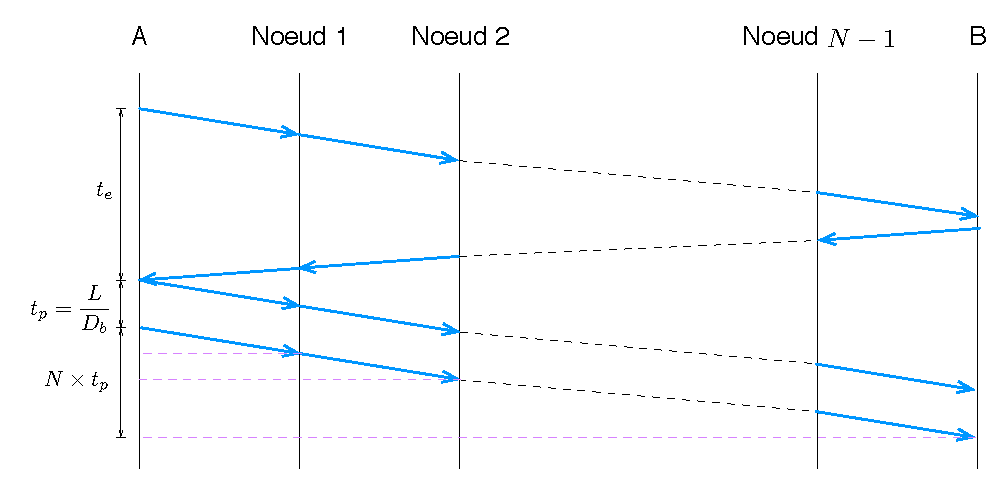
\includegraphics[scale=.7]{graphes/CC}
	\caption{Commutation de circuit}
\end{figure}

\subsection{Commutation de messages} % (fold)

\begin{def*}[Message]
	Suite d'information formant un tout pour l'expéditeur et le destinataire.
	
	Messages envoyés indépendamment les uns des autres.\\
	Commutateur : \emph{store and forward} -- reçoit, stocke le message dans une file d'attente et le vérifie avant de le renvoyer vers le port de sortie approprié.
\end{def*}

\begin{description}
	\item [Avantage] Permet d'utiliser les ressources du réseau uniquement lorsque c'est nécessaire.\\
	$\Rightarrow$ Echanges variables, sporadiques ou par rafale.
	\item[Inconvénients] \hfill \begin{itemize}
		\item Le message n'étant pas de taille bornée, il faudra des sources importantes de stockage;
		\item Temps de transfert importants à cause de la technique \emph{store and forward};
		\item Mécanisme de contrôle nécessaire pour éviter les congestions;
		\item Du fait de leur taille parfois importante les messages on une forte probabilité de contenir des erreurs. En cas d'erreur le message entier doit être retransmis.
		\end{itemize}
\end{description}

Temps de transfert d'un message sur $N$ noeuds :
\[
	T_{M}=\frac{L+E_{m}}{D_{b}}+t_{p}+\left(t_{r}+\frac{L+E_{m}}{D_{b}}+t_{p}\right)\left(N-1\right)
\]

\begin{figure}[h!]
	\center
	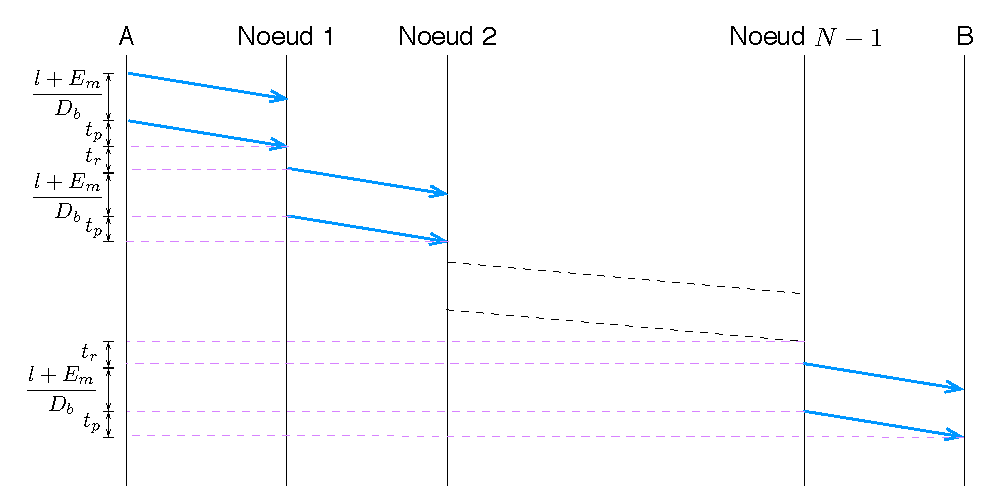
\includegraphics[scale=.75]{graphes/CM}
	\caption{Commutation de messages}
\end{figure}

\subsection{Commutation de paquets} % (fold)

\begin{def*}[Paquet]
	Message de taille limitée (bornée à 1500, 2000 octets).
	
	Le message à transmettre est découpé en paquets de données. Un paquet contient :\begin{itemize}
		\item Une portion du message découpé;
		\item Origine, destination du message;
		\item Indication sur le réassemblage du message.
	\end{itemize}
\end{def*}

\begin{figure}[h]
	\center
	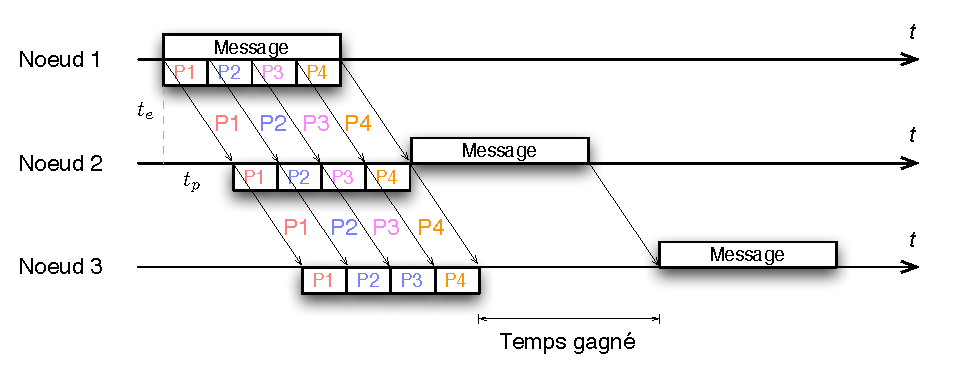
\includegraphics[scale=.75]{graphes/CV-CC}
	\caption{La commutation de message vs. la commutation de paquets}
\end{figure}

\paragraph{Mode connecté - circuit virtuel (CV)} % (fold)
eg. X.25
\begin{itemize}
	\item Etablissement du CV -- réservé par le billet des voies logiques;
	\item Les paquets vont alors suivre le même chemin dans le réseau.
	\item Les paquets arrivent dans le bon ordre.
\end{itemize}

Temps de transfert d'un paquet en mode CV sur $N$ noeuds :
\[
	T_{CV}=\begin{cases}
		t_{e}+\left(\frac{l+E_{p}}{D_{b}}+t_{p}\right)N+\left(\frac{l+E_{p}}{D_{b}}\right)\left(q-1\right) & \textrm{si }r=0\\
		t_{e}+\left(\frac{l+E_{p}}{D_{b}}+t_{p}\right)N+\left(\frac{l+E_{p}}{D_{b}}\right)\left(q-1\right)+\frac{r+E_{r}}{D_{b}} & \textrm{si }r\ne0
	\end{cases}
\] avec $L=l\times q+r$ et $0\leqslant r<l$

\paragraph{Mode non connecté - datagramme} % (fold)
eg. IP
\begin{itemize}
	\item Les paquets sont indépendants les uns des autres. Ils ne vont pas suivre le même chemin dans le réseau.\\
	$\Rightarrow$ Déséquencement
	\item La station réceptrice devra alors rassembler les paquets dans le bon ordre pour reconstituer le message.
\end{itemize}

Temps de transfert d'un paquet en mode datagramme sur $N$ noeuds :
\[
	T_{D}=\begin{cases}
	\left(\frac{l+E_{p}}{D_{b}}+t_{p}\right)+\left(t_{r}+\frac{l+E_{p}}{D_{b}}+t_{p}\right)\left(N-1\right)+\left(\frac{l+E_{p}}{D_{b}}\right)\left(q-1\right) & \textrm{si }r=0\\
	\left(\frac{l+E_{p}}{D_{b}}+t_{p}\right)+\left(t_{r}+\frac{l+E_{p}}{D_{b}}+t_{p}\right)\left(N-1\right)+\left(\frac{l+E_{p}}{D_{b}}\right)\left(q-1\right)+\frac{r+E_{r}}{D_{b}} & \textrm{si }r\ne0\end{cases}
\] avec $L=l\times q+r$ et $0\leqslant r<l$


\begin{description}
	\item [Avantages]\hfill\begin{itemize}
		\item Permet de résoudre efficacement les erreurs de transmission, seul le paquet erroné (et non le message entier) va être retransmis;
		\item Diminution du temps de transfert en augmentant le parallélisme;
		\item Cela permet de multiplexer temporellement sur une même liaison les paquets appartenants à plusieurs messages.
	\end{itemize}
	\item [Inconvénients]\hfill\begin{itemize}
		\item Un dé-séquancement peut être introduit en mode non connecté;
		\item Risque de congestion;
		\item Délai d'acheminement/transfert variable.
	\end{itemize}
\end{description}

\begin{figure}[h!]
	\center
	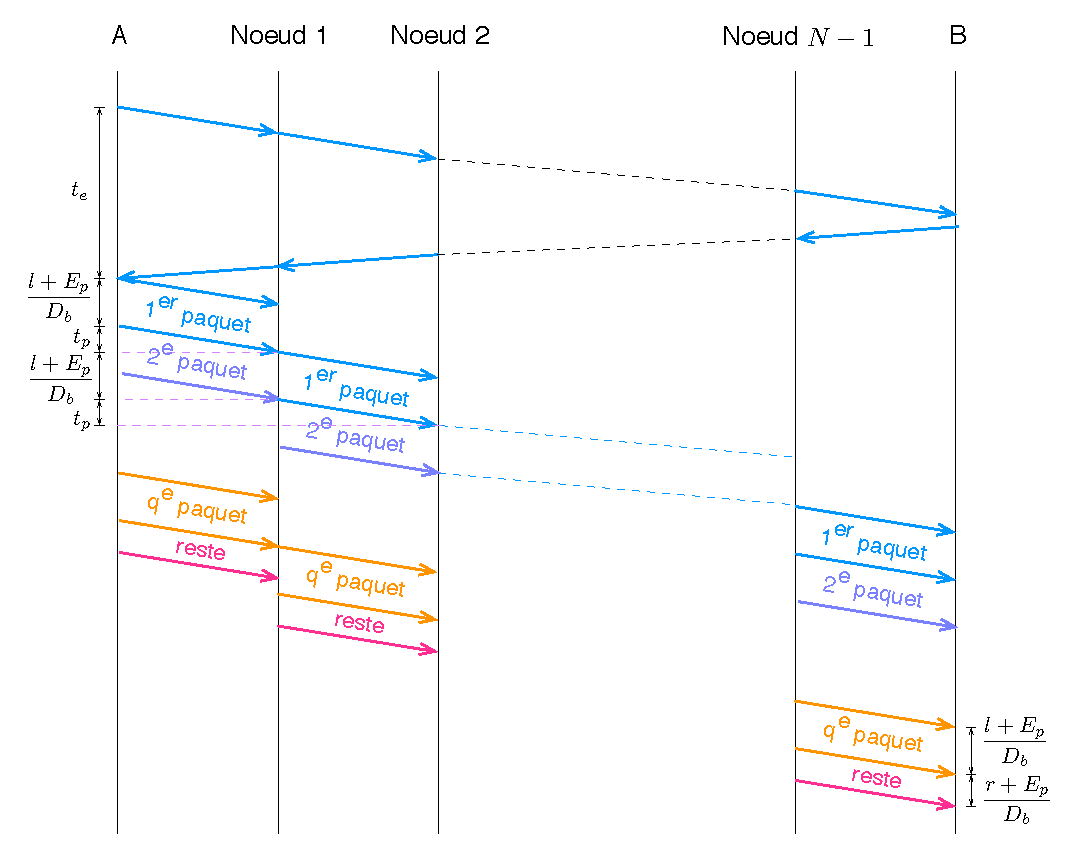
\includegraphics[scale=.75]{graphes/CPCV}
	\caption{Commutation de paquets (mode CV)}
\end{figure}

\begin{figure}[h!]
	\center
	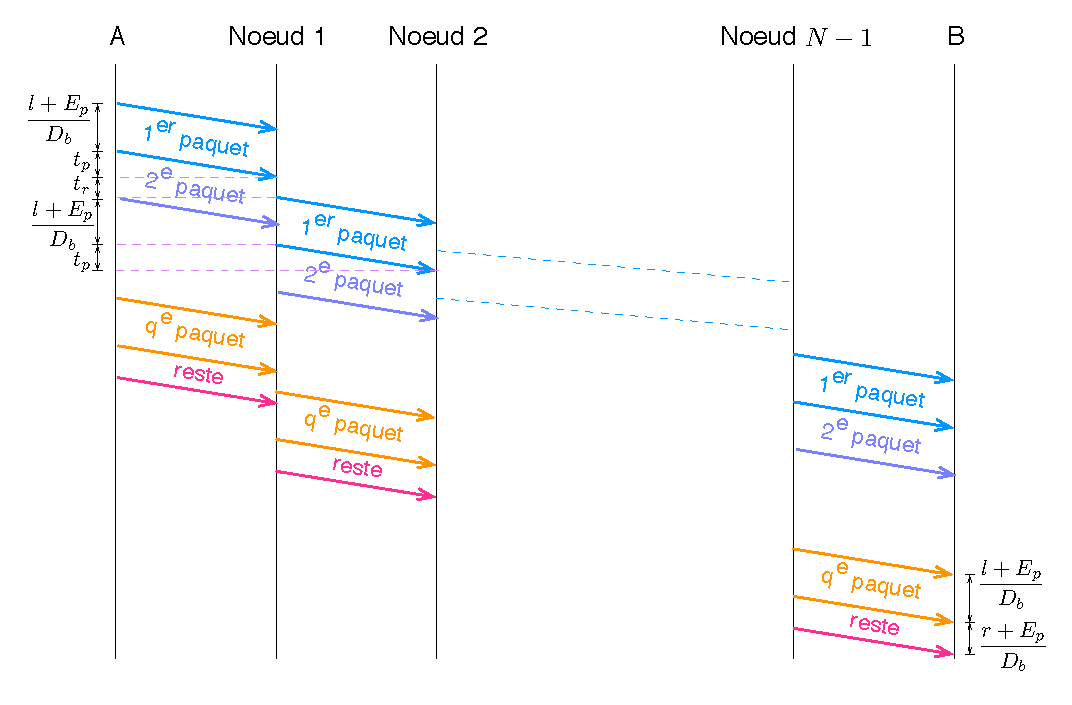
\includegraphics[scale=.75]{graphes/CP}
	\caption{Commutation de paquets (mode datagramme)}
\end{figure}


\subsection{Commutation de cellules} % (fold)

\begin{def*}[Cellule]
	Une cellule a pour caractéristiques :\begin{itemize}
		\item Une taille fixe;
		\item Une petite taille (eg. cellule ATM : 53 octets)
	\end{itemize}
\end{def*}

\begin{description}
	\item [Avantages -- taille fixe]\hfill\begin{itemize}
		\item Augmentation de la capacité des noeuds;
		\item Meilleures performances (utilisation de circuit électronique préprogrammé);
		\item Gestion mémoire des commutateurs plus simple.
	\end{itemize}
	\item[Inconvénient -- taille fixe] Mauvaise utilisation de la bande passante : le cadrage des cellules va nécessiter des octets de bourrage.
	\item[Avantages -- petite taille] \hfill\begin{itemize}
		\item Réduction du temps de constitution des paquets/unités de données (de cellules);
		\item Réduction du délai/temps d'acheminements grâce au parallélisme;
		\item Réduction du nombre de perte et de la taille de tampon des noeuds;
		\item Meilleurs entrelacement des messages;
		\item Gigue(écart type du temps de transfert) faible (environ 100 $\mu$s).
	\end{itemize}
	\item[Inconvénients -- petite taille] \hfill\begin{itemize}
		\item Diminution de l'efficacité de transmission car chaque cellule comporte un entête $\Rightarrow$ \emph{overhead} (débit) important;
		\item Augmentation de traitements dans les noeuds de commutation.
	\end{itemize}
\end{description}

\clearpage

\section{Multiplexage statique} % (fold)

Le coût d'installation et de maintenance d'un lien entre deux éléments de commutation est le même pour des artères ayant une large bande passante que pour des liens de faible bande passante. 

D'où l'idée du multiplexage permettant de regrouper plusieurs communications simultanées (des conversations dans le cas d’un réseau téléphonique) sur un même lien physique.

 Les matériels qui réalisent cette juxtaposition ont pour rôle de regrouper les informations de plusieurs circuits de données sur un seul circuit, appelé \textbf{circuit composite}.

\begin{figure}[h!]
	\center
	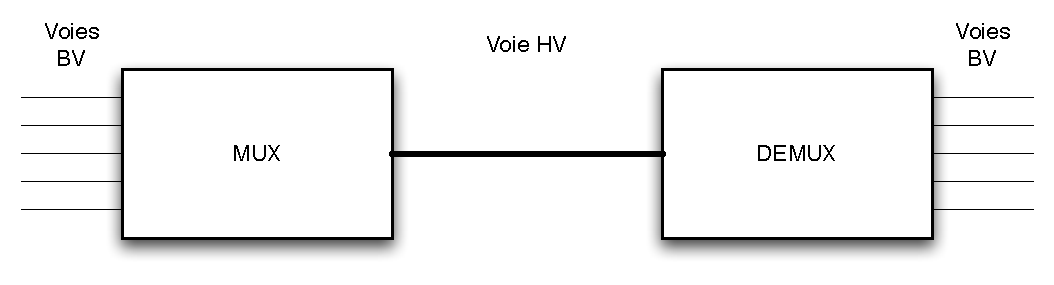
\includegraphics[scale=.75]{graphes/multiplexage}
	\caption{Principe du multiplexage}
\end{figure}

\begin{def*}[Multiplexage]
	Le multiplexage statique consiste à partager, par une méthode invariable dans le temps, le débit binaire $D_b$ d'une voie haute vitesse (HV) entre plusieurs voies basse vitesse (BV) ou canaux. 
\end{def*}

\begin{rem*}
	La somme des débits $D_i$ des voies BV ne peut excéder le débit $D_b$ de la voie HV. Le multiplexeur va combiner plusieurs voies BV en un seul train de données sur la ligne HV.
\end{rem*}

Il existe deux modes de multiplexage :\begin{itemize}
	\item Le multiplexage fréquentiel;
	\item le multiplexage temporel.
\end{itemize}

Ces deux modes de multiplexage consistent à découper la voie HV en différents canaux, chacun
étant associé à une voie BV.

\begin{def*}[Signalisation]
	En plus des données, un circuit composite doit pouvoir transmettre d'autres informations relatives à chaque circuit multiplexé. Ces informations sont appelées \textbf{signalisations}. 
	
	Deux méthodes sont possibles pour la transmission des signalisations :\begin{itemize}
		\item La \textbf{signalisation dans la bande} : la signalisation est transmise sur les différents canaux, à la place des données;
		\item La \textbf{signalisation hors bande} : la signalisation est transmise sur un canal séparé, appelé canal sémaphore.
	\end{itemize}	
\end{def*}

\begin{rem*}
	Il est à noter que même si le multiplexage fréquentiel n’est plus beaucoup utilisé dans les réseaux filaires, ceux-ci utilisant de plus en plus la transmission numérique, il reste une technique très employée dans les réseaux sans fils (GSM).
	Il existe par ailleurs un mode de multiplexage très proche du multiplexage fréquentiel, le
	multiplexage en longueur d’onde. Celui-ci s’applique sur une fibre optique et consiste à partager la plage de longueurs d’ondes de la fibre en sous-bandes de longueur d’ondes disjointes.
\end{rem*}

\subsection{Multiplexage fréquentiel (FDM)} % (fold)

Le multiplexage fréquentiel (Multiplexage par Répartition en Fréquence ou \emph{Frequency Division Multiplexing}) est principalement utilisé dans les systèmes analogiques (réseau téléphonique). 

Il consiste à partager la bande de fréquences disponible en un certain nombre de canaux (ou sous-bandes) plus étroits et à affecter en permanence chacun de ces canaux à une communication exclusive.

\begin{figure}[h!]
	\center
	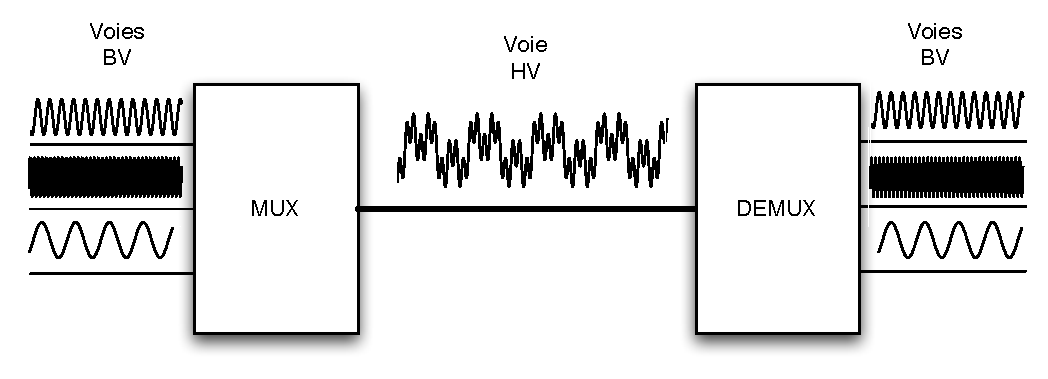
\includegraphics[scale=.75]{graphes/multiplexage-frequentiel}
	\caption{Principe du multiplexage fréquentiel}
\end{figure}

\subsection{Multiplexage temporel (TDM)} % (fold)

Le multiplexage temporel (Multiplexage par Répartition dans le Temps ou \emph{Time Division Multiplexing}) est mieux adapté aux signaux numériques. 

\begin{figure}[h!]
	\center
	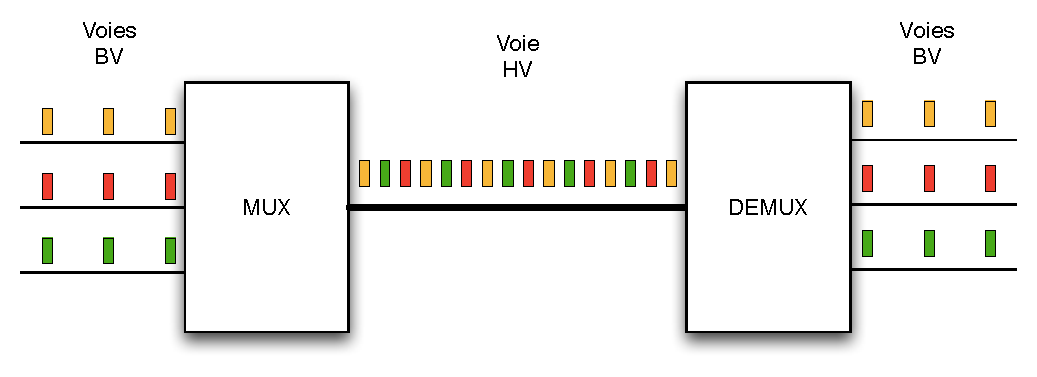
\includegraphics[scale=.75]{graphes/multiplexage-temporel}
	\caption{Principe du multiplexage temporel}
\end{figure}

Le partage des ressources se fait dans le temps. La totalité de la capacité du canal composite est allouée à un canal de communication pendant une tranche de temps fixe à intervalles réguliers. 

\begin{def*}[Intervalle de temps (IT)]
	Le multiplexeur manipule des \textbf{intervalles de temps} (IT) ou \emph{time-slot} contenant des prélèvements d'unités de données de chaque canal. Ces IT sont regroupés en une suite bornée nommée \textbf{trame multiplexée} ou \textbf{multiplex}. Cette structure de trame est répétée avec une certaine fréquence. 
\end{def*}

\begin{rem*}
	Un IT est réservé à chaque canal de communication qui a la même position à l'intérieur de 2 multiplex quelconques.
\end{rem*}

\begin{figure}[h!]
	\center
	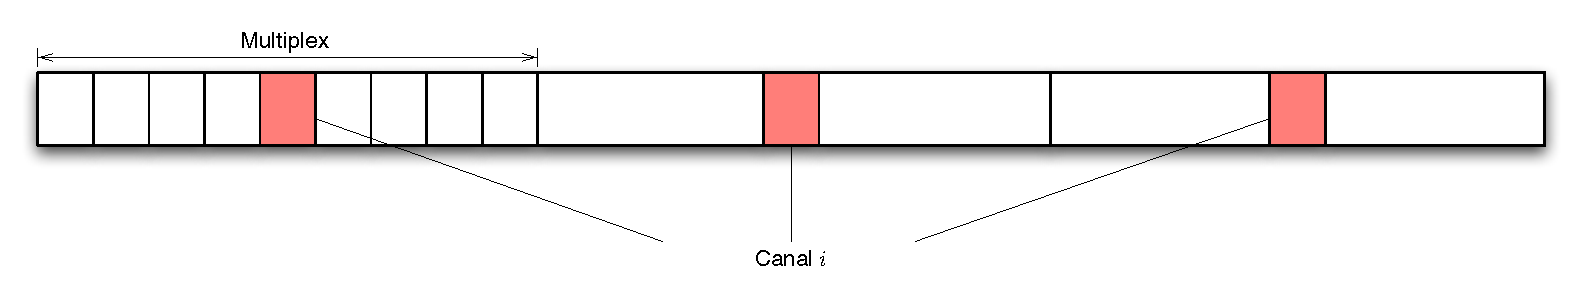
\includegraphics[scale=.5]{graphes/multiplex-temporel}
	\caption{Un multiplex temporel}
\end{figure}

\begin{def*}[Verrouillage de trame]
	Le premier IT de chaque trame n'est affecté à aucun canal : il transmet une combinaison particulière appelée \textbf{verrouillage de trame}, qui sert à reconnaître le début d'une trame et à maintenir la synchronisation entre les deux multiplexeurs.
\end{def*}

\subsubsection{Multiplexage par bits / par caractères} % (fold)

On considère un train numérique permanent de débit $D_b$ bit/s. On découpe le train en trames de $L$ bits : 
\begin{figure}[h!]
	\center
	\vspace{-25pt}
	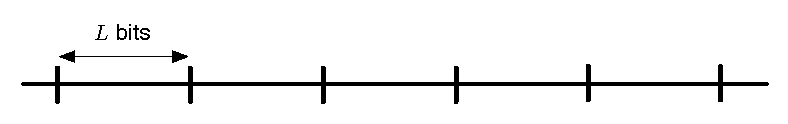
\includegraphics[scale=.75]{graphes/train-trame}
	\vspace{-15pt}
\end{figure}

Chaque trame est ensuite découpée en intervalles de temps (IT) :
\begin{figure}[h!]
	\center
	\vspace{-15pt}
	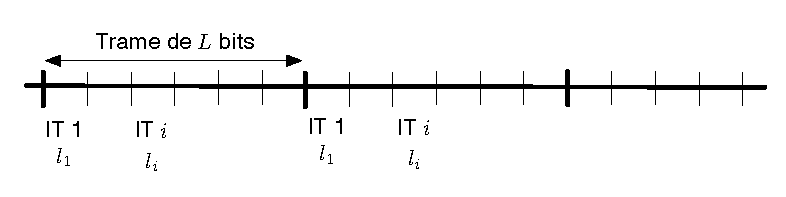
\includegraphics[scale=.75]{graphes/intervalle-temps}
	\vspace{-15pt}
\end{figure}

Dans un mode de \textbf{multiplexage par caractères}, chaque IT i a une longueur de $l_i$ bits. Les différents IT peuvent avoir des longueurs différentes, mais les IT ayant la même position ($i$) à l'intérieur de deux trames quelconques ont la même longueur :
\[L=\sum_i l_i\]

Le \textbf{rythme} (ou \textbf{cadence}) de répétition (ou d'occurrence) des trames est : 
\[R=\frac{D}{L}\qquad\textrm{trame/s}\]

La succession des IT de numéro $i$ des différentes trames constitue un circuit de données appelé
canal N°$i$. Le débit binaire du canal $i$ sur la voie HV est : 
\[d_i=\frac{l_i}{L}D\qquad\textrm{bit/s}\]

Le principe du \textbf{multiplexage par bits} est similaire excepté que la longueur de chaque IT est de 1 bit.

\subsubsection{Voies BV asynchrones / synchrones} % (fold)

\begin{def*}[Voies BV asynchrones]
	Lorsque les voies BV sont \textbf{asynchrones}, la transmission sur la voie BV n’est pas synchronisée : les horloges de l’émetteur et du récepteur (le multiplexeur) sont indépendantes. 
\end{def*}

\begin{rem*}
	L’unité de données sur une voie BV asynchrone est le caractère.
	
	La délimitation des caractères sur la voie BV doit donc être assurée par des bits supplémentaires : chaque caractère commence par un bit de \emph{Start} et se termine par un (ou plusieurs) bit(s) de \emph{Stop}. 
	
	Sur la voie HV, seule l’information utile (sans les bits \emph{Start} et \emph{Stop}) est transmise.
\end{rem*}

\begin{def*}[Voies BV synchrones]
	Lorsque les voies BV sont \textbf{synchrones}, la transmission sur la voie BV est synchronisée entre
	l’émetteur de la voie et le récepteur (le multiplexeur) à l’aide d’une horloge commune (obtenue par la transmission d’un signal de temps sur la ligne).
\end{def*}

\begin{rem*}
	Cette synchronisation permet de ne transmettre sur une voie BV que l’information utile, sans bit supplémentaire.
\end{rem*}

\begin{def*}[Efficacité d'un multiplexeur]
	L'efficacité $e$ d'un multiplexeur est donnée par :
	\[e=\frac{\sum_i C_i N_i}{D_b}\]
	\begin{itemize}
		\item $C_i$ est la rapidité de transfert en car/s de la voie BV $i$ (Basse Vitesse $i$);
		\item $N_i$ est le nombre de bits utiles par caractère (sans bit \emph{Start} ni \emph{Stop});
		\item $D_b$ est le débit en bit/s de la voie HV (Haute Vitesse).
	\end{itemize}
	
	L’efficacité $e$ s’interprète comme le rapport du débit utile (nombre de bits de données à transmettre sur la voie HV par unité de temps et provenant des voies BV), sur le débit maximum de la voie HV.	
\end{def*}

\section{Normes de multiplexage dans les artères de commutation} % (fold)

Pour utiliser un mode de multiplexage temporel dans les réseaux téléphoniques, il faut convertir les signaux analogiques en signaux numériques. Cette numérisation s’effectue dans les commutateurs locaux et requiert des codecs (codeur/décodeurs). Il existe différentes techniques de numérisation : \emph{Pulse Code Modulation}, \emph{Differential Pulse Code Modulation}, \emph{Delta Modulation}, etc. 

La Modulation par Impulsion et Codage, \emph{MIC} (PCM - \emph{Pulse Code Modulation}), échantillonne le signal à une fréquence de 8000 Hz (ce qui correspond à un échantillon toutes les 125 $\mu$s) et code chaque échantillon sur 8 bits. Le débit engendré est donc de 64 kbit/s.

Originellement il fût impossible d’obtenir une norme internationale de multiplexage, aussi plusieurs standards coexistent.

\paragraph{Canal E1 (Europe)} % (fold)

Le canal E1 est largement répandu en dehors des US et du Japon, et a été normalisé par l’IUT sous la norme G.732. Ce standard repose sur une numérisation par modulation MIC, et utilise des IT de 8 bits et une signalisation hors bande.

\begin{figure}[h!]
	\center
	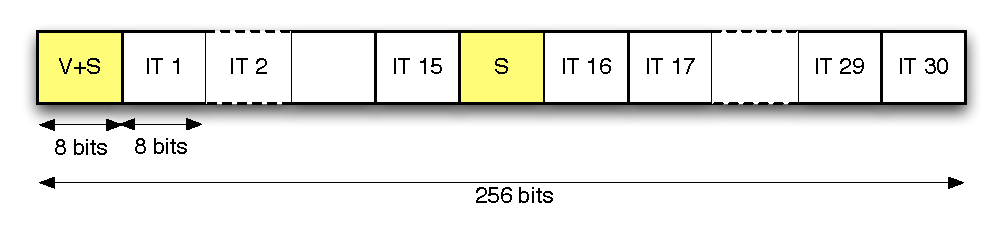
\includegraphics[scale=.75]{graphes/multiplex-E1}
	\caption{Le multiplex E1}
\end{figure}

Les trames sont émises toutes les 125 $\mu$s et contiennent chacune 32 IT de 8 bits (numérotées de 0 à 31), dont 30 IT pour les données et 2 IT pour le verrouillage et la signalisation (les IT N° 0 et N° 16). L’IT N° 0 est alternativement consacré au verrouillage (trames impaires) et à la signalisation (trames paires) tandis que l’IT N° 16 est entièrement consacré à la signalisation.
Le multiplexage est temporel, seul mode possible pour les messages numériques. 


Les trames sont émises toutes les 125 $\mu$s, ce qui correspond à une fréquence de 8000 Hz.
On a  L'efficacité du multiplexage est égal à 30/32.


\chapter{Les réseaux} % (fold)

\section{Rôle d'un réseau} % (fold)

\begin{def*}[Réseau]
	Le réseau est un temporisateur: son rôle est d'acheminer des données de leur source à leur destination. Les données qui pénètrent dans le réseau en provenance d'une station sont routées vers leur destinataire en étant commutées de nœud en nœud. Certains nœuds ne sont reliés qu'à d'autres nœuds du réseau: leur seule tâche est alors la commutation interne.
	D'autres (les nœuds d'accès) sont également reliés à des stations: en plus de la fonction de commutation, ils doivent pouvoir accepter des données en provenance des utilisateurs du réseau et, réciproquement, leur délivrer des données.	
\end{def*}

Du point de vue de deux stations communicantes, le réseau peut donc être considéré comme une généralisation d'une liaison point-à-point. Mais les fonctionnalités assurées par une liaison de données ne sont pas suffisantes pour permettre l'acheminement de données entre un ETTD source et un ETTD destinataire, trois fonctions sont absentes:
\begin{description} 
\item [L'adressage] Pour délivrer un paquets à un destinataire il faut connaître sont adresse ce qui implique de définir un mécanisme d'adressage.
\item [Le routage] Consiste à déterminer la route que le paquet devra emprunté dans le réseau. Cela pose 3 questions:\begin{itemize}
	\item Quels sont les critères de choix pour trouver la bonne route;
	\item Quel algorithme appliquer pour calculer les routes (eg. Dijkstra);
	\item Comment échanger les informations nécessaire au calcule des routes ? ce qui va ce faire par le protocole de routage.
	\end{itemize}
\item [Le contrôle de congestion]
\end{description}
On ajoute donc des fonctionnalités qui n'étaient pas disponible au niveau liaison.

Deux approches sont possibles.

\section{Service en mode connecté (circuit virtuel)} % (fold)
Analogie : le téléphone.

La communication se divise en trois phases :\begin{description}
	\item [Etablissement de la connexion virtuel] Identification des entités en communication, négociation tripartite (les deux ETTD et le réseau), détermination de la route qui seras emprunté par tous les paquets de la connexion (cela ce fait par un paquet d'appel qui comporte les adresse de l'appelant et de l'appelé qui trace la route), réservation des ressources de communication;
	\item [Transfert de données] Avec un volume d'information de contrôle minimisé;
	\item [Libération des ressources de communication]
\end{description}

Ce service est considéré comme \textbf{fiable} : les paquets qui appartiennent à une connections sont référencé et il est possible de faire un contrôle de flux, un contrôle d'erreur et un contrôle de séquence. C'est l'approche que fournissait l'opérateur France Telecom\texttrademark.

\section{Service en mode non connecté (datagrame)} % (fold)
Analogie : la poste.

Les paquets sont indépendants les un des autres il n'y a pas de phase d'établissement ni libération de la connexion. 

Transfert de données direct :les datagrames sont indépendant les un des autres, chaque paquets est considéré par le réseau comme une entité propre, chaque paquets peut éventuellement choisir un trajets différents des autres et donc des délais de transferts différents et donc une réception dé-séquencé. Chaque paquet doit contenir toute l'information de contrôle, notamment d'adressage (ce qui prend de la place) nécessaire à son acheminement.

\begin{itemize}
	\item Ce service est considéré comme \textbf{non fiable}, souvent qualifié comme \emph{best effort}.
	\item Le séquencement des données n'est pas garanti.
	\item Le contrôle de flux est très difficile, il peut y avoir des erreurs des pertes et duplication de paquets sont possible.
\end{itemize}

\begin{conc*}
	Le réseau est peu fiable, c'est à l'usager d'effectuer tous les contrôles. Le réseau fourni un service minimum (\emph{best effort}). C'est l'approche Internet.
\end{conc*}

\section{Interface X.25} % (fold)
\subsection{Généralités} %(fold)

La recommandation X.25 a été adopté par l'ITU-T en 1976. Protocole proposé à l'origine par les PTT françaises, les PTT britanniques, le canadien Trans Canada Telephone System et l'américain Telenet Communication Corps, il a été implanté sur les réseaux publics des ces quatre compagnies (Transpac, EPSS, Datapac et Telenet).

X.25 offre un service de réseau en \emph{\textbf{mode connecté}} et spécifie une \textbf{interface d'accès} à un réseau à commutation de paquets: il s'agit donc d'une interface locale entre un équipement connecté au réseau et le réseau lui-même, entre un ETTD et un ETCD.

\begin{figure}[h!]
	\center
	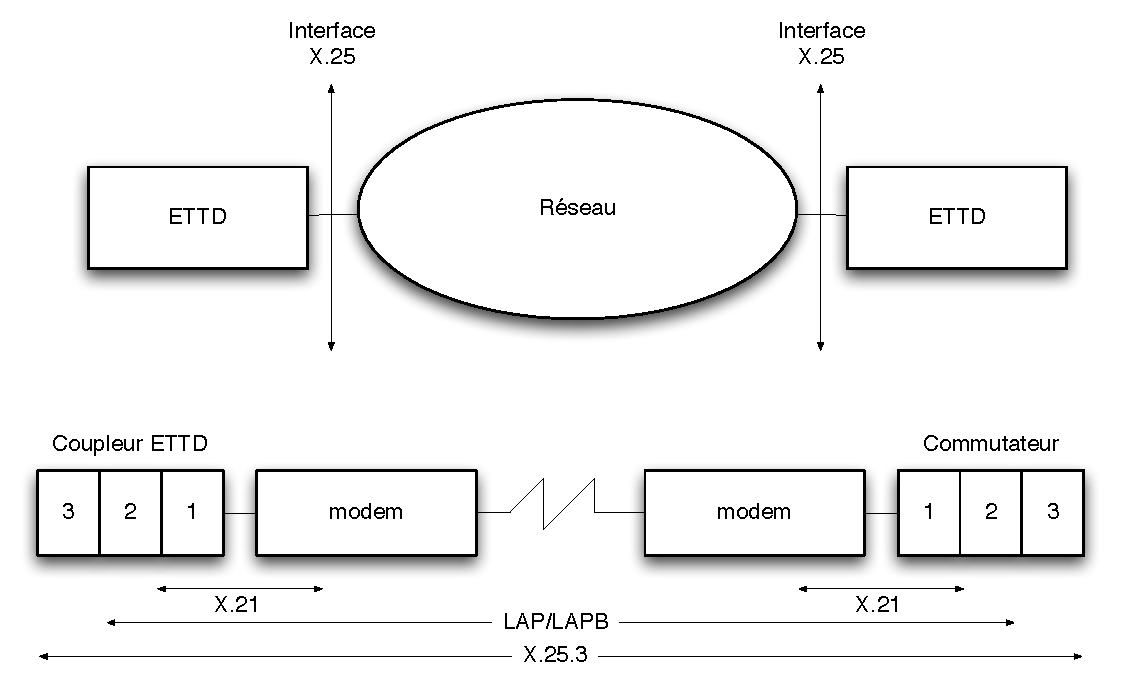
\includegraphics[scale=.65]{graphes/X25}
	\caption{Interface d'accès X.25}
\end{figure}

X.25 contient trois niveaux de protocoles:
\begin{description}
	\item[Un niveau physique]: interface conforme à la norme X.21 ou X.21 bis, solution intérimaire qui permet de se connecter à un réseau public numérique à partir d'un équipement utilisant l'interface V.24 (V.24 ayant été conçu à l'origine pour l'interface avec des réseaux de télécommunications analogiques);
	\item[Un niveau liaison]LAP-B = sous-ensemble de la procédure HDLC (en mode ABM);
	\item[Un niveau réseau]X.25 niveau paquet (PLP \emph{Packet Level Protocol}) gère le transfert de paquets d'une station source vers une station destinataire; l'unité d'information y est le \textbf{paquet} :
	\begin{itemize}
		\item tout paquet est placé dans le champ d'information d'une trame I (\textbf{encapsulation});
		\item la longueur de ce champ limite la longueur du paquet;
		\item par convention, il ne peut y avoir plus d'un paquet par trame.
	\end{itemize}
\end{description} 

X.25 définit les types de paquets et leur format, mais ne spécifie pas comment certaines informations de contrôle doivent être interprétées (eg. la fenêtre de contrôle de flux). Ces imprécisions ont donné naissance à des réseaux conformes à X.25, mais différents dans leur implantation.

\subsection{Le niveau réseau PLP: circuit virtuel et voie logique}

X.25 supporte un service de réseau en \textbf{\emph{mode connecté}} on parle également de \textbf{\emph{circuit virtuel}} (CV). Les deux partenaires en communication ont l'illusion d'un canal point-à-point dédié. La connexion correspond à une association bidirectionnelle entre les deux ETTD. 

Deux types de circuits virtuels sont possibles : 
\begin{description}
	\item[CVP (Circuit Virtuel Permanent)] Un CVP relie en permanence deux (mêmes) abonnés; l'établissement du CV est fait pour toute la durée de l'abonnement.
	\item[CVC (Circuit Virtuel Commuté)] Un CVC permet à un abonné d'atteindre tout autre abonné, tout transfert de données doit être précédé d'une phase d'établissement et doit se terminer par une phase de libération du CVC.
\end{description}


\begin{def*}[Voie logique]
	La notion de voie logique (VL) permet la coexistence de tronçons de plusieurs CV sur une même liaison, c'est un moyen de transmission bidirectionnelle simultanée sur une liaison de données. Elle est identifiée par un N° de GVL (groupe de VL) $\le 15$ et un numéro de VL $\le 255$ 
	(signification purement locale à l'interface), donc globalement sur 12 bits. Ces valeurs sont attribuées à l'abonnement dans le cas d'un CVP et lors de l'établissement pour un CVC.
\end{def*}

\begin{rem*}
	Un circuit virtuel est une connexion de bout en bout, alors que le numéro de voie logique est un identifiant local du circuit virtuel, on peut voir un circuit virtuel comme une succession de numéro de voie logique sur chaque liaison emprunté.
	
	$2^{12} = 4096$ circuits virtuels peuvent, au plus, transiter entre deux noeuds.
\end{rem*}

\begin{figure}[h!]
	\center
	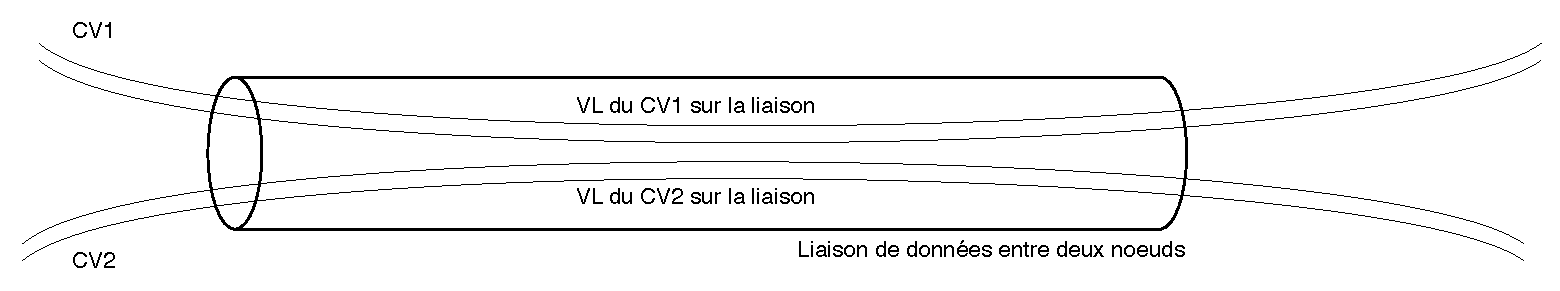
\includegraphics[scale=.7]{graphes/VL}
	\caption{Voies logiques (VL)}
\end{figure}

Le multiplexage des VL sur une même liaison se traduit par un entrelacement de paquets appartenant à des CV différents dans les trames qui circulent sur la liaison de données.

\begin{figure}[h!]
	\center
	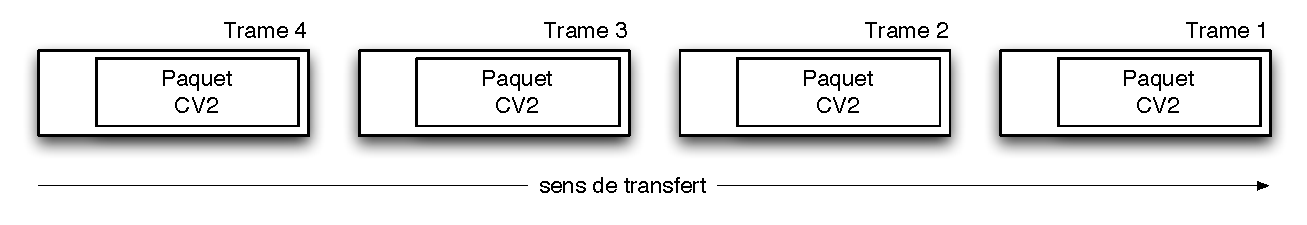
\includegraphics[scale=.7]{graphes/multiplexage-paquets}
	\caption{Multiplexage sur une VL}
\end{figure}

\subsection{Le niveau réseau PLP: Les paquets X.25}

Chaque paquet transféré à travers l'interface comporte au moins trois octets contenant: 
\begin{itemize}
	\item Une identification générale de format : indique entre autres le modulo utilisé (8 ou 128);
	\item Une identification de voie logique : N° GVL et N° VL;
	\item Une identification de type de paquet.
\end{itemize}

\begin{rem*}
	Il est à noter que seuls les paquets d’appel et d’appel entrant contiennent nécessairement l’adresse source (ETTD appelant) et l’adresse destination (ETTD appelé).
\end{rem*}

\subsection{Le niveau réseau PLP : Les différentes phases d'un circuit virtuel}

\subsubsection*{Etablissement d'un CVC} % (fold)

\begin{figure}[h!]
	\center
	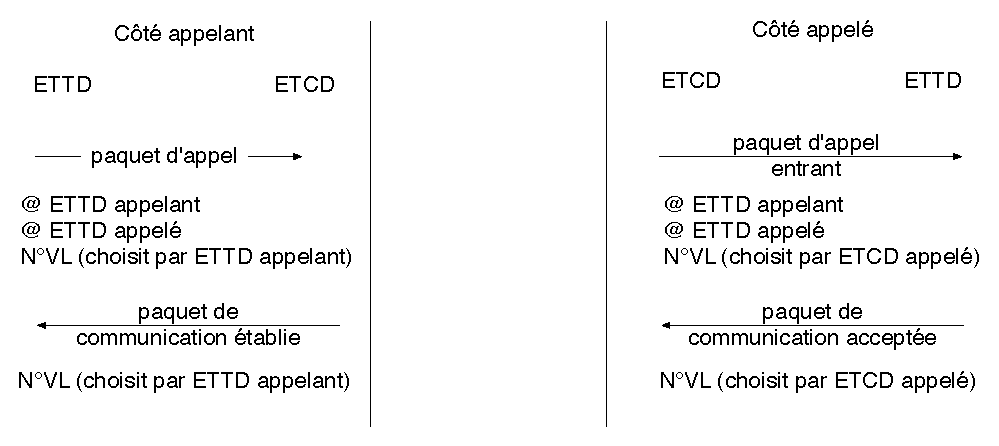
\includegraphics[scale=.7]{graphes/X25-etablissement}
	\caption{Etablissement d'une connexion circuit virtuel permanent}
\end{figure}


En cas de refus de l'ETTD appelé, celui-ci envoie un paquet de demande de libération à l'ETCD appelé qui provoquera l'envoi par l'ETCD appelant d'un paquet d'indication de libération. 

En cas de collision d'appel sur une interface, lorsque l'ETTD et l'ETCD transmettent en même temps un paquet d'appel et un paquet d'appel entrant indiquant le même numéro de voie logique, l'ETCD traite le paquet d'appel et ne tient pas compte du paquet d'appel entrant, toutefois, l'ETTD distant reçoit une indication de libération.
Afin de minimiser les risques de collision d'appels, et par convention, l'ETTD choisit comme numéro de voie logique (N° GVL + N° VL) le plus grand numéro disponible, alors que l'ETCD choisira le plus petit possible.

\clearpage

\subsubsection*{Transfert de données} % (fold)

Les paquets utilisés pendant cette phase sont :

\begin{figure}[h!]
	\center
	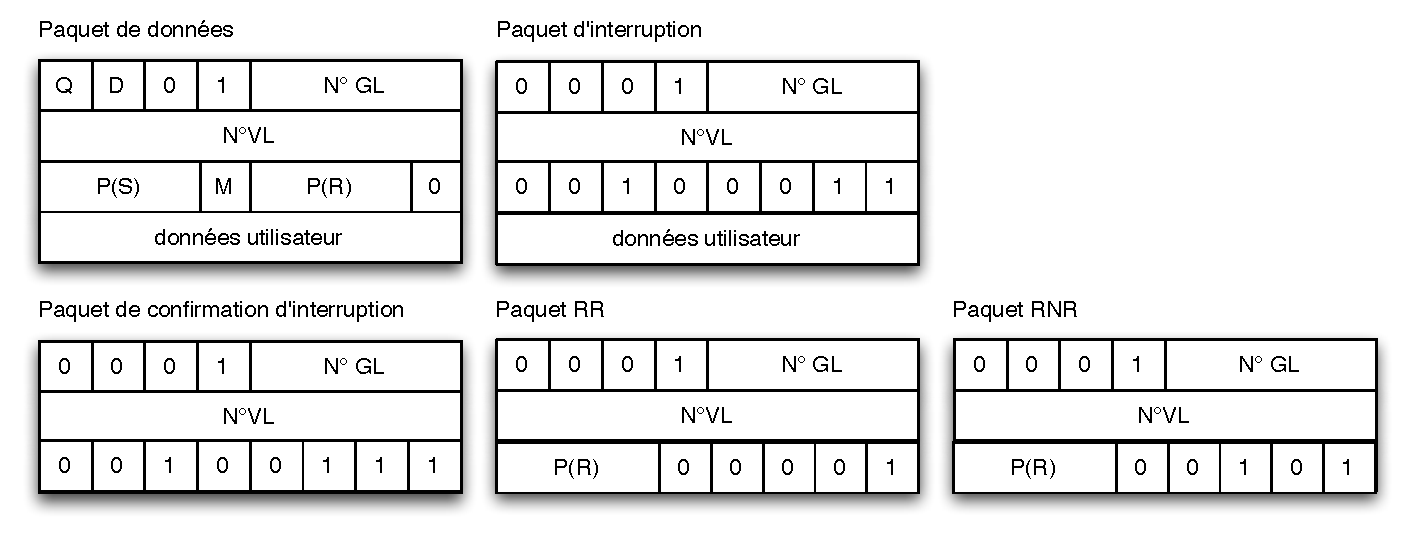
\includegraphics[scale=.7]{graphes/paquets-X25}
	\caption{Paquets X.25}
\end{figure}

Dans le paquet de données:
\begin{itemize}
	\item $Q$ est le bit de qualification des données. Dans certains cas l'usager peut souhaiter différencier deux types d'information dans les paquets de données, par exemple les données de l'usager et l'information de commande;
	\item $D$ est le bit de portée de l'acquittement :\begin{itemize}
		\item si $D = 0$, l'acquittement se fait par l'ETCD local;
		\item si $D = 1$, l'acquittement est de bout en bout (il est alors généré par l'ETTD distant).
	\end{itemize}
	\item 01 indique une numérotation modulo 8 (10 pour un modulo 128);
	\item $P(S)$ est le numéro de séquence du paquet;
	\item $M$ est la marque ``données à suivre''. Ce bit est utilisé par un ETCD ou un ETTD s'il souhaite indiquer une séquence comportant plus d'un paquet, le dernier paquet de la séquence a le bit M à 0, les autres le bit M à 1;
	\item $P(R)$ est le numéro de séquence en réception (\emph{piggybacking});
	\item La longueur maximale normalisée du champ de données est de 128 octets.
\end{itemize}


Le paquet d'interruption est un paquet comportant entre 1 et 32 octets de données, non numéroté, non soumis au contrôle de flux, et qui doit être acquitté par un paquet de confirmation d'interruption. Il sert à transporter des informations urgentes. A tout moment un ETTD ne peut avoir plus d'un paquet d'interruption en attente d'acquittement.


\subsubsection*{Contrôle de flux} % (fold)

Le contrôle de flux au niveau des paquets utilise, comme au niveau de la liaison, un mécanisme de fenêtrage. A l'interface ETTD/ETCD, une fenêtre est définie pour chaque sens de transmission, dont la taille $W$ normalisée est de 2 (cette taille peut être négociée lors de la phase d'établissement, il s'agit cependant d'un service optionnel facturé à l'usager). De façon similaire à HDLC, un paquet de données doit, pour pouvoir être émis, avoir son $P(S)$ à l'intérieur de la fenêtre :
\[
	\textrm{dernier } P(R) \textrm{ reçu} \leqslant P(S) \leqslant \textrm{dernier } P(R) \textrm{ reçu} + W - 1
\]

\begin{rem*}
La fenêtre de niveau liaison indique le nombre de trame I qu'un émetteur peut émettre sans acquittement, alors que la fenêtre de niveau réseau donne le nombre de paquets qui peuvent être envoyés sans acquittement.

Les deux fenêtres sont gérées par des couches différentes, toutefois la fenêtre de niveau liaison doit être la plus grande possible dans le cas contraire il y aurait toujours blocage au niveau liaison avant qu'il n'y ait blocage sur le circuit virtuel.
\end{rem*}

\subsubsection{Libération de CVC} % (fold)

\begin{figure}[h!]
	\center
	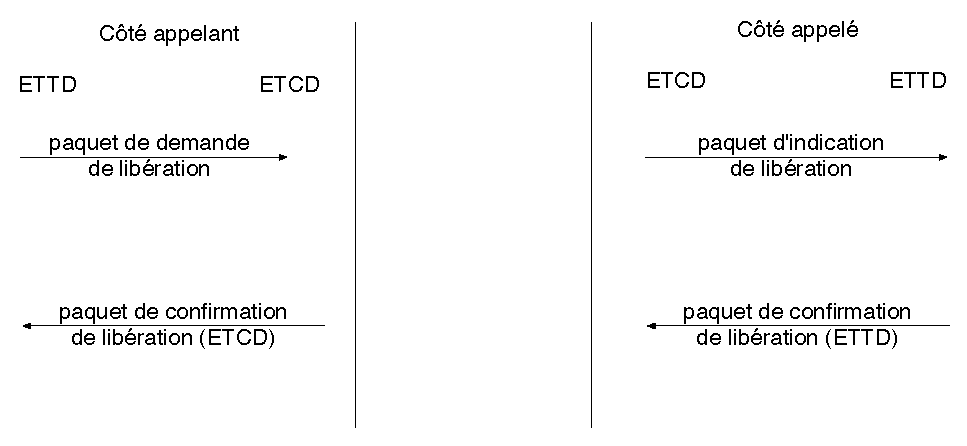
\includegraphics[scale=.7]{graphes/X25-liberation}
	\caption{Libération d'une connexion circuit virtuel permanent}
\end{figure}

\begin{figure}[h!]
	\center
	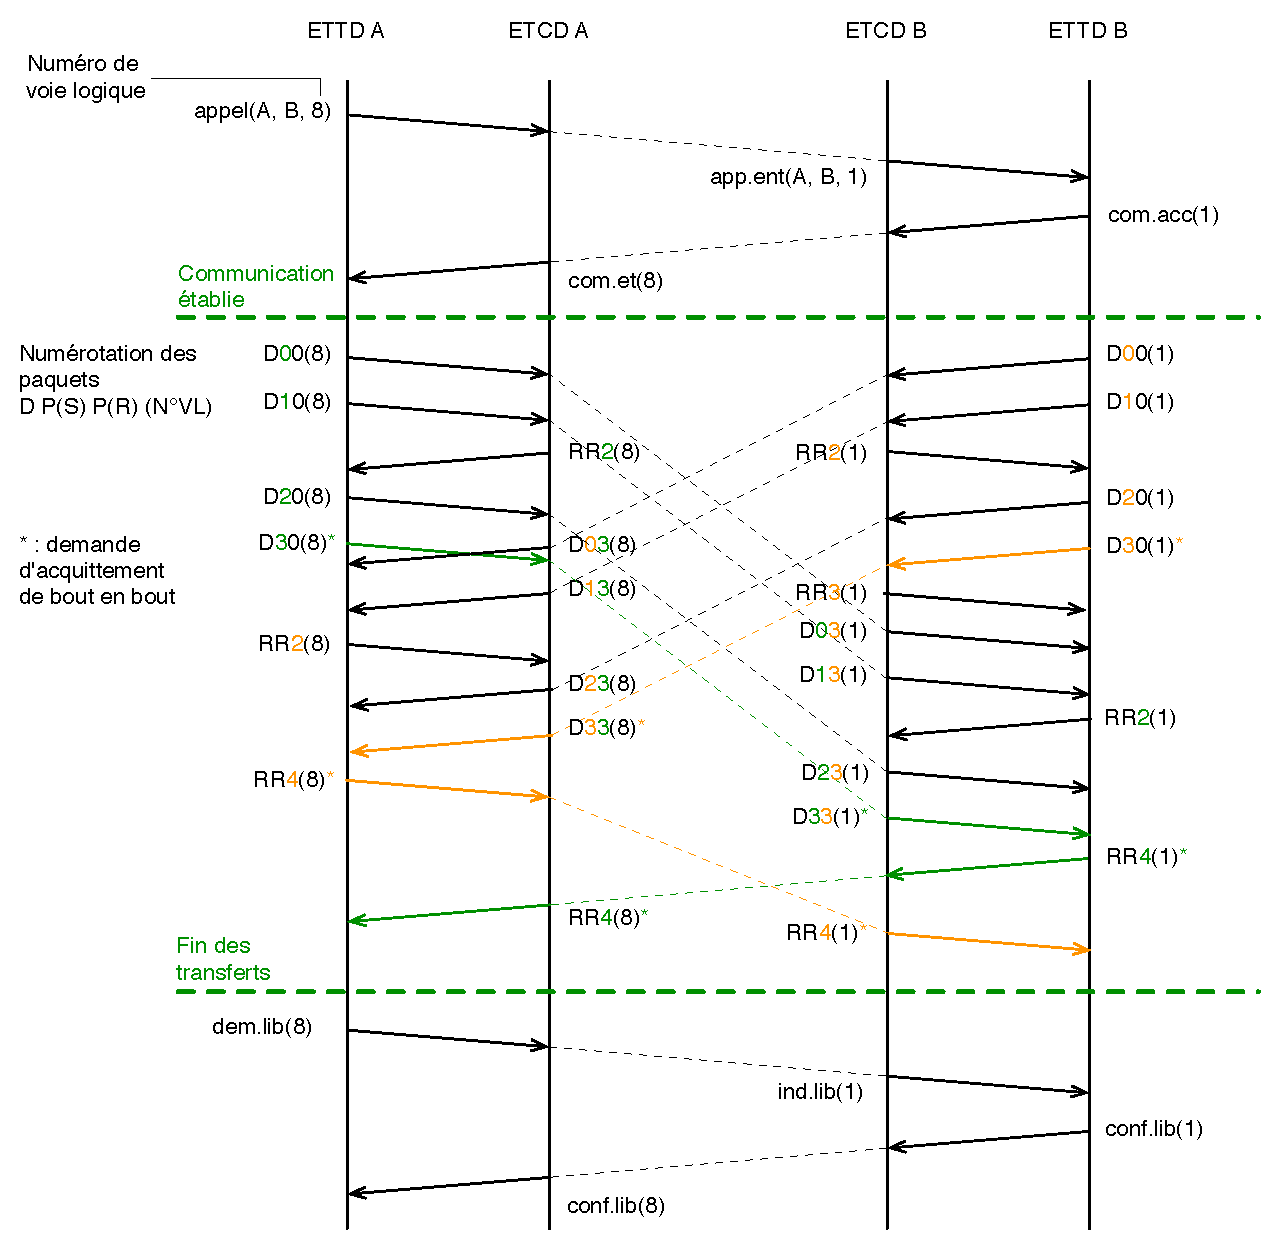
\includegraphics[scale=.75]{graphes/echange-paquets1}
	\caption{Echange de paquets entre ETTD et ETCD}
\end{figure}

\begin{figure}[h!]
	\center
	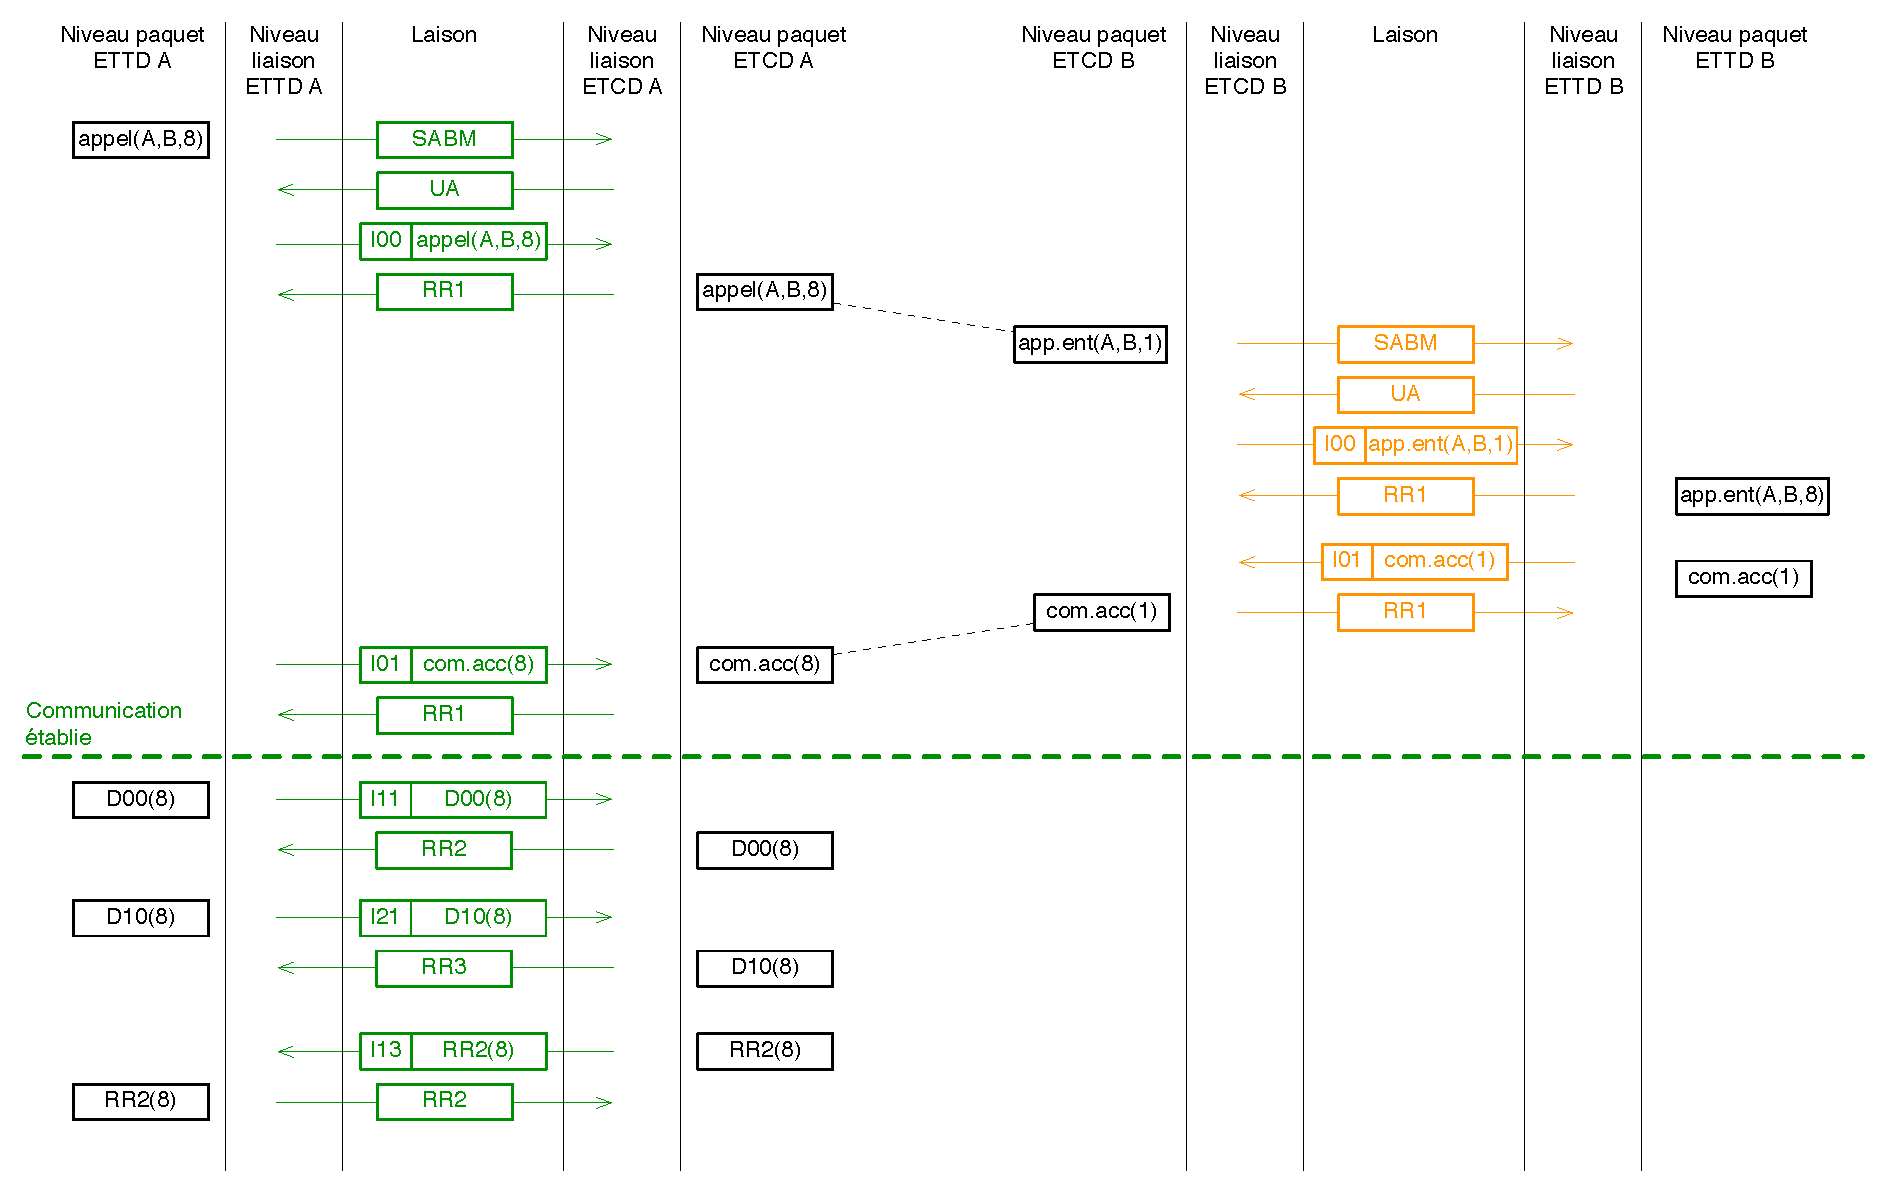
\includegraphics[scale=.5]{graphes/echange-paquets2}
	\caption{Echange de paquets entre ETTD et ETCD}
\end{figure}

\chapter{Routage} % (fold)

\section{Généralités} % (fold)

\begin{def*}[Routage]
	Le routage est le processus qui consiste, dans un réseau, ou au travers de différents réseaux, à \textbf{trouver un chemin entre une source et une destination}. C'est l'une des fonctionnalités principales de la couche réseau. On appelle \textbf{\textit{routeur}} un équipement relié à au moins deux réseaux et dont le rôle est de réémettre des paquets venus d'une de ses interfaces vers une autre.
\end{def*}

	Schématiquement, on peut représenter l'Internet comme une hiérarchie de routeurs.
	
\begin{def*}[Système autonome]
	On appelle \textbf{\textit{système autonome}} (\textit{Autonomous System} ou AS) un ensemble de routeurs et de réseaux contrôlés par une même autorité administrative: on peut donc voir l'Internet comme un ensemble d'AS. 
	Deux types de routage :\begin{itemize}
		\item Routage intra-domaine (IGP -- \emph{Interior Gateway Protocol}) :  routeurs situés à l'intérieur d'un même AS;
		\item Routage inter-domaine (EGP -- \emph{Exterior Gateway Protocol}) : routeurs qui permettent de relier entre eux différents AS.
	\end{itemize}
\end{def*}
	
	Le routage (intra-domaine) est réalisé grâce aux \textbf{protocoles de routage} qui maintiennent des \textbf{tables de routage} dans les routeurs ( et commutateurs) du réseau. 
	
	Une table de routage comporte au moins deux colonnes: \begin{itemize}
		\item destination (ou pour le réseau de destination);
		\item adresse de l'élément réseau correspondant au ``saut'' suivant (\textit{next hop}) sur le ``meilleur'' chemin vers la destination souhaitée.
	\end{itemize}
	
	Lorsqu'un paquet arrive sur un routeur (ou lorsqu'un paquet d'appel arrive sur un commutateur), le routeur (le commutateur) consulte sa table de routage pour décider du prochain saut pour ce paquet.

Le moment de prise de décision du routage (consultation de la table de routage) dépend du mode d'acheminement :\begin{description}
	\item[Acheminement par voie logique]\hfill\begin{itemize}
	 	\item décision prise une seule fois lors du passage du paquet d'établissement;
		\item tous les autres paquets de la connexion suivent la même route, après consultation de la table de translation.
	\end{itemize}
	\item[Par datagramme]\hfill\begin{itemize}
	 	\item une décision de routage est prise pour chaque paquet;
		\item la route peut être identique ou non pour deux paquets ayant le même destinataire.
	\end{itemize}
\end{description}

Tout protocole de routage doit communiquer des informations sur la topologie globale du réseau à chaque routeur afin que celui-ci puisse prendre une décision locale de routage. Or, cette information globale est difficile à collecter, sujette à des modifications fréquentes et de plus, volumineuse. 

Un ``bon'' protocole de routage visera donc :\begin{itemize}
	\item Une minimisation des messages de contrôle échangés
	\item Une minimisation de l'espace des tables de routage : \begin{itemize}
		\item minimiser le coût des routeurs;
		\item minimiser le trafic d'information de routage (puisque les routeurs s'échangent leurs tables de routage pour garantir une vue consistante de la topologie du réseau).
	\end{itemize}
	\item La robustesse : éviter les trous noirs, les boucles et les oscillations;
	\item L'utilisation du chemin ``optimal'' qui n'est pas forcément le plus court : il peut s'agir du chemin au délai le plus court, du chemin le plus sécurisé, du chemin le moins cher, ou tout simplement du chemin utilisant le moins de sauts.
\end{itemize}

\vspace{10pt}
	
Le routage est par essence, un problème de la \textbf{théorie des graphes}: il s'agit de trouver le chemin du coût minimum entre deux nœuds quelconques, sachant que le coût d'un chemin est la somme des coûts des liens qui le composent.

Il existe plusieurs classes de techniques de routage :\begin{description}
	\item[Le routage isolé] Cette classe regroupe des techniques qui ne nécessitent aucun échange d'information entre les nœuds et ne construisent pas de table de routage. (eg. le \emph{le routage par inondation} dans lequel chaque nœud retransmet toujours tous les paquets sur toutes ces interfaces, sauf l'interface entrante).
	\item[Le routage centralisé] On dispose d'un centre de contrôle de routage qui reçoit périodiquement des informations décrivant l'encombrement du réseau. Il en déduit les tables de routage de chaque routeur et les leur expédie.
	\item[Le routage distribué] Chaque routeur échange périodiquement des informations avec ses voisins et recalcule sa table de routage. Deux types d'algorithmes de routage distribué sont largement utilisés :\begin{itemize}
		\item \textbf{Le routage à vecteurs de distance} (eg. \emph{Routing Information Protocol} ou RIP);
		\item \textbf{Le routage à états des liens} (eg. \emph{Open Shortest Path First} ou OSPF).
	\end{itemize}
\end{description}

Les algorithmes à vecteurs de distance et à états des liens partagent des caractéristiques communes:\begin{itemize}
	\item ils supposent que chaque routeur connaît l'adresse de chacun de ses voisins, ainsi que le ``coût'' pour l'atteindre;
	\item ils permettent à chaque routeur de déterminer l'information de routage globale (ie. le prochain nœud pour atteindre chaque destination possible sur la route la plus courte, en échangeant de l'information de routage seulement avec ses voisins).
\end{itemize}
	
\section{Algorithme à vecteurs de distance} % (fold)

\subsection{Principe} % (fold)

L'algorithme de base est dû à \textbf{Bellman-Ford}. Chaque nœud est supposé connaître la ``distance'' (ou le «coût») qui le sépare de chacun de ses voisins (une liaison hors service a un coût infini). Périodiquement, chaque nœud envoie à chacun de ses voisins la liste des distances estimées vers chaque nœud du réseau: c'est le \emph{\textbf{vecteur de distance}}. Il reçoit parfois une liste similaire de chacun de ses voisins.
\newline

Lorsque le nœud $i$ reçoit le vecteur de distance $V_j$ de son nœud voisin $j$, $V_j(k)$ lui donne la distance (estimée par $j$) pour aller de $j$ à $k$, et il sait donc qu'il peut atteindre $k$ via $j$, avec un coût de $V_j(k)$ augmenté du coût de sa liaison à $j$. en poursuivant ce calcul pour chacun de ses voisins, $i$ peut déterminer l'estimation qui lui semble la meilleure pour atteindre chaque destination, et inscrire cette estimation ainsi que la liaison correspondante dans sa table de routage.
\newline

Plusieurs solutions permettent de pallier le problème du comptage à l'infini:\begin{description}
	\item[Le vecteur de chemin] Chaque entrée du vecteur de distance contient le chemin complet associé à la valeur. C'est une technique utilisée dans BGP, mais qui présente l'inconvénient de générer des tables volumineuses. (Il est à noter que BGP, \emph{Border Gateway Protocol}, est un protocole de routage inter-AS);
	\item[L'horizon partagé (\emph{split horizon})] Un routeur ne communique jamais le coût vers une destination à son voisin N, si N est le prochain nœud vers cette destination;
	\item[L'horizon partagé avec antidote (\emph{split horizon with poisonous reverse})] Un routeur communique toujours un coût infini vers une destination à son voisin $N$, dés l'instant où $N$ est le prochain nœud vers cette destination. Cela se traduit par une modification mineure du protocole de vecteurs de distance: au lieu de diffuser le même vecteur sur toutes leurs liaisons, les nœuds devront en composer des versions différentes, pour tenir compte des destinations qui sont atteintes via chacune de ces liaisons. C'est la technique utilisée dans le RIP.
\end{description}

\begin{rem*}
	L'horizon partagé est efficace pour éviter le comptage à l'infini lorsqu'on a une boucle entre 2 routeurs (efficace dans le sens où elle accélère la convergence), mais elle ne l'est pas lorsqu'on a 3 routeurs ou plus dans la boucle.
\end{rem*}

\begin{rem*}
	La plupart des algorithme prévoient d'envoyer les vecteurs de distances de façon périodique. Cependant, il est souhaitable de signaler aussitôt que possible des pannes, les vecteurs de distance reportant une panne de noeud ou de lien sont immédiatement envoyés (donc de façon asynchrone).
\end{rem*}

\section{Algorithme de routage à effets de liens} % (fold)

\subsection{Principe} % (fold)

Dans cette approche, un routeur communique à tout autre nœud du réseau sa distance avec ses voisins. En effet, l'idée est de distribuer les topologies et le coût de chaque lien à tous les routeurs ? chaque routeur peut alors calculer de façon autonome, son chemin optimum pour chaque destination. Si les routeurs voient les mêmes coûts pour tous les liens et s'ils utilisent le même algorithme, les routes obtenues sont garanties sans boucle. Le problème est donc de distribuer la connaissance de la topologie à chaque routeur pour qu'il puisse ensuite calculer ses plus courts chemins.

Chaque routeur doit ainsi:\begin{enumerate}
	\item \emph{Découvrir ses voisins}
	
	Un routeur en cours d'initialisation envoie sur chacune de ses lignes en sortie un paquet \lstinline!Hello!, les routeurs aux extrémités répondront à ce paquet en retournant des informations de routage (ID, adresse IP, etc).
	\item \emph{Mesurer le coût vers chacun des voisins}	
	
	Si le coût est basé sur le temps d'acheminement, le routeur peut en obtenir une bonne estimation en envoyant un paquet \lstinline!Echo! estampillé et en prenant la moitié du temps aller-retour.
	\item \emph{Construire un paquet spécial}
	
	Le routeur crée un ensemble de LSP (\emph{Link-State Packet}) décrivant ses liens. Un LSP contient l'ID du routeur, l'ID du voisin et le coût du lien vers ce voisin.
	\item \emph{Envoyer ce paquet à tous les autres routeurs du réseau}
	
	Ceci, est fait par inondation contrôlée. L'idée est lorsqu'un routeur reçoit un nouveau LSP, il en garde une copie dans sa base de données de LSP et il le retransmet sur chacune de ses voies de sorties (sauf celle sur laquelle le LSP lui est parvenu).
	\item \emph{Calculer le plus court chemin vers tous les autres routeurs}
	
	L'\textbf{algorithme de Dijkstra} calcule le chemin le plus court entre un sommet source $s$ et tous les autres sommets d'un graphe $G = (S,\,A)$ valué par une fonction de pondération $\omega \colon A \rightarrow \mathbb{R}$.
	
	On définit:\begin{itemize}
		\item $E$ : le sous-ensemble des sommets déjà évalués (pour lesquels les chemins les plus courts sont connus);
		\item $R$ : le sous-ensemble des sommets restants ($R = S \backslash E$);
	\end{itemize}
	
	Pour chaque sommet $v \in S$, on maintient deux attributs:\begin{itemize}
		\item $d[v]$ : l'estimation du coût d'un plus court chemin de $s$ à $v$;
		\item $\textrm{pred}[v]$ : le prédécesseur de $v$ sur le chemin estimé.
	\end{itemize}
\end{enumerate}

\section{Routage et commutation} % (fold)

Un commutateur est un équipement permettant d'interconnecter des liaisons de façon à former un réseau. Cet équipement, possédant plusieurs ports en entrée et plusieurs ports en sortie, a pou rôle de transférer un paquet qu'il reçoit sur un port d'entrée vers un port de sortie. La question qui se pose est alors de savoir comment le (bon) port de sortie est déterminé. La réponse se trouve dans l'en-tête d'un paquet, deux approches sont possibles: \begin{description}
	\item [Commutation en mode non connecté (datagramme)] Le paquet est réacheminé sur la base de son adresse de destination;
	\item [Commutation en mode connecté (circuit virtuel)] Le paquet est réacheminé sur la base de son identificateur de circuit virtuel.
\end{description}

\chapter{Réseaux Locaux, Techniques d'accès} % (fold)

\section{Topologies} % (fold)

Un réseau est un système qui relie entre eux des postes de travail. La manière de relier les stations définit la \textbf{\emph{topologie physique}} (encore appelée \textbf{\emph{plan de câblage}}). Elle est à distinguer de la \textbf{\emph{topologie logique}} (encore appelée \textbf{\emph{topologie d'accès}}), qui décrit la façon dont circule “logiquement” l'information. La topologie est celle prise en compte par la \textbf{\emph{méthode d'accès}}.

Il existe plusieurs types de topologies (physiques). Le choix de l'une ou de l'autre sera influencé par la vitesse à laquelle on souhaite travailler, par la disposition des lieux, par le type de câble que l'on veut utiliser ou qui est déjà installé et par le coût.

Toutes les architectures réseaux dérivent de trois topologies fondamentales:\begin{description}
	\item [Bus] : les ordinateurs sont connectés les uns à la suite des autres le long d'un seul câble (segment). Le bus est une topologie passive: les ordinateurs qui y sont connectés (et qui n'ont pas de données à transmettre) ne font qu'``écouter'' les données qui circulent sur le réseau. Le retrait des informations aux deux extrémités est implicite et s'effectue grâce aux terminateurs en fin de bus qui évitent les problèmes de réflexion du signal arrivant à l'extrémité du support;
	\item [Etoile] : les ordinateurs sont connectés à des segments de câble qui partent tous d'un même point, le \emph{concentrateur} ou \emph{contrôleur central}. Celui-ci gère l'accès au support;
	\item [Anneau] : les ordinateurs sont connectés à un câble qui forme une boucle. Chaque ordinateur fait office de répéteur en amplifiant le signal qui lui parvient afin de l'envoyer à l'ordinateur suivant.
\end{description}


Ces trois topologies de base sont simples en elles-mêmes. Toutefois, les topologies utilisées dans la pratique combinent souvent les caractéristiques de plusieurs d'entre elles, et peuvent donc s'avérer plus complexes.

Ces topologies ont des propriétés identiques de diffusion et de partage du support:\begin{itemize}
	\item toutes les stations peuvent lire les données qui transitent sur le support;
	\item toutes les stations peuvent écrire sur le support.
\end{itemize}

\subsection{Bus} % (fold)

\begin{description}
	\item [Avantages]
	\begin{itemize}
		\item facile à installer;
		\item retrait implicite des informations (grâce aux terminateurs en fin de bus qui évitent les problèmes de réflexion du signal arrivant à l'extrémité du support), contrairement à l'anneau, où c'est à l'émetteur de retirer sa propre information lorsqu'elle a fait un tour complet;
		\item topologie passive. si un ordinateur tombe en panne, cela n'a pas d'incidence sur le reste du réseau.
	\end{itemize}
	\item [Inconvénients]
	\begin{itemize}
		\item risques de collisions (ou contention d'accès) si deux signaux sont émis simultanément, se superposent et deviennent incompréhensibles (cacophonie), d'où un temps d'accès indéterministe;
		\item les unités d'accès sont passives, le signal n'est donc pas régénéré. La taille du segment est donc limitée ( à cause de l'atténuation). La taille peut  être augmentée en ajoutant des répéteurs entre les segments;
		\item lien multipoint non adapté à la fibre optique (support unidirectionnel) et complexe à maintenir;
		\item en cas de rupture du câble coaxial commun, le réseau sera dit hors service car il y aura alors “rebond” du signal aux 2 nouvelles extrémités créées (sauf si l'on ajoute deux bouchons de terminaisons).
	\end{itemize}
\end{description}

\subsection{Etoile} % (fold)

\begin{description}
	\item [Avantages]
	\begin{itemize}
		\item conflits d'accès réglés en central;
		\item technologie simple et éprouvée: topologie classique des réseaux téléphoniques avec le PABX (\emph{Private Auto Branch eXchange})= contrôleur qui relie toutes les machines;
		\item les pannes d'une machine sont gérées simplement en déconnectant la branche de la machine en cause;
		\item liens point à point: on peut utiliser la fibre optique.
	\end{itemize}
	\item [Inconvénients]
	\begin{itemize}
		\item problèmes de fiabilité du nœud central ( en cas de panne aucune transmission n'est possible);
		\item la taille du réseau (le nombre de stations) dépend de la puissance du contrôleur central;
		\item si le réseau est grand, cette topologie exige davantage de câblage.
	\end{itemize}
\end{description}

\subsection{Anneau} % (fold)

\begin{description}
	\item [Avantages]\hfill
	\begin{itemize}
		\item pas de taille limite au réseau (chaque station est connectée à l'anneau - lien en boucle unidirectionnel - par un répéteur);
		\item liens point à point adaptés à la fibre optique et simples à maintenir;
		\item temps de transfert borné.
	\end{itemize}
	\item [Inconvénients]\hfill
	\begin{itemize}
		\item retrait des informations nécessaire;
		\item problèmes de fiabilité si l'anneau se coupe (ce problème peut être pallié en doublant l'anneau);
		\item les connecteurs sont complexes et coûteux;
		\item la gestion des pannes est difficiles : dans la mesure où le signal passe par tous les ordinateurs, une panne d'un ordinateur peut avoir une incidence sur l'ensemble du réseau.
	\end{itemize}
\end{description}

Le partage du support est arbitré par des mécanismes appelés \emph{\textbf{méthodes d'accès}} ou \emph{\textbf{protocoles d'accès}} ou encore \emph{\textbf{politiques d'accès}}. Il existe deux grandes classes de méthodes d'accès: 
\begin{itemize}
	\item Les méthodes d'accès statiques;
	\item Les méthodes d'accès dynamiques; parmi ces dernières, on fait la distinction entre:
	\begin{itemize}
		\item Les méthodes à allocation déterministes;
		\item Les méthodes à allocation aléatoire.
	\end{itemize}
\end{itemize}

\section{Politiques d'accès statiques} % (fold)

Les méthodes d'accès statiques consistent à partager de façon statique (donc sans évolution dans le temps) les ressources de transmission (abusivement appelées “bande passante”) entre plusieurs communicateurs. Il existe deux façons simples d'effectuer ce partage: \begin{description}
	\item [AMRF]  (Accès multiple à répartition en fréquence) : la bande passante du support physique est découpée en sous-bandes dont chacune est affectée à un seul communicateur;
	\item [AMRT]  (Accès multiple à répartition dans le temps) : Le temps est découpé en tranches (appelés \emph{Intervalle de Temps} ou IT), que l'on affect successivement aux différents communicateurs.\\
\end{description}

\begin{description}
	\item [Avantages] \hfill
	\begin{itemize}
			\item ces techniques sont simples et efficaces si le nombre de stations est fixe;
			\item elles sont équitables entre les stations et permettent un accès régulier au support;
			\item elles permettent d'implémenter simplement des mécanismes de priorité.
	\end{itemize}
	\item[Inconvénients] \hfill
	\begin{itemize}
		\item si une station n'a rien à émettre il y a un gâchis de bande passante;
		\item pour l'AMRT: il est nécessaire de “synchroniser” les stations. Cette synchronisation doit être mise en place par une station primaire qui doit gérer les ajouts ou les retraits de stations sur le réseau. Il se pose donc des problèmes de fiabilité lorsque la station primaire est en panne.
		\item pour l'AMRF: le découpage en sous-bandes introduit des inter-bandes (afin d'éviter au maximum les interférences), d'où un gâchis de la bande passante. Chaque station a besoin d'autant de démodulateurs qu'il  a de sous-bandes afin de pouvoir recevoir de tous les émetteurs.
	\end{itemize}
\end{description}



\begin{rem*}
	Ces techniques semblent peu adaptées aux réseaux locaux en effet :
	\begin{itemize}
		\item elles sont peu flexibles dès l'instant où le nombre de stations varie;
		\item si toutes les stations n'émettent pas il y a un gâchis de bande passante qui limite les stations qui ont envie d'émettre.
	\end{itemize}
	
	Il est à noter cependant que les techniques de multiplexage sont largement utilisées dans les réseaux longue distance (WAN).
\end{rem*}

\section{Politiques d'accès dynamiques à allocation déterministes} % (fold)

Ces techniques d'allocation permettent de n'allouer des ressources ( de la “bande passante”) qu'aux utilisateurs qui en ont réellement besoin. La difficulté provient du manque de connaissance des besoins utilisateurs à tout instant. Cela nécessite donc la mise en place d'une “intelligence”, celle-ci pouvant être centralisée ou répartie entre les utilisateurs.

\subsection{Politiques d'accès à allocation sélective ou \emph{polling} (solution centralisée)}

Cette technique d'allocation d'une ressource unique (le canal) entre plusieurs compétiteurs consiste à effectuer une consultation des divers compétiteurs en les invitant à émettre à tour de rôle. Une \emph{\textbf{station centrale}} (encore appelée \emph{\textbf{site maître}}), qui peut être soit une machine soit un concentrateur de terminaux,, gère l'ensemble du système en interrogeant séquentiellement chaque station, afin de voir si elle a des trames à émettre. En cas de réponse positive, la station transmet sa trame au site maître qui, ultérieurement, interrogera la station destinataire pour savoir si elle est prête à recevoir, et lui enverra alors les données en cas de réponse positive. On distingue deux variantes:
\begin{description}
	\item [Roll-call polling] (topologie logique en étoile) : la station primaire interroge successivement chacune des stations secondaires en lui envoyant une \emph{\textbf{trame de poll}}. La station interrogée lui répond par une trame d'acquittement négatif si elle n'a rien à lui envoyer ou par une trame de données dans le cas contraire;
	\item [Hub polling] (topologie logique en bus) : la station primaire démarre un cycle en envoyant une trame de poll à la station secondaire “la plus éloignée” sur le bus. Si cette dernière a des données à émettre, elle les lui envoie puis elle envoie une trame de poll à la station secondaire “suivante” sur la liaison. Dans le cas contraire, elle envoie immédiatement la trame de poll à la station secondaire suivante. La “dernière” station secondaire envoie une trame de poll au primaire qui démarre un nouveau cycle.
\end{description}

\begin{description}
	\item[Avantages] \hfill
	\begin{itemize}
			\item la technique du polling est simple à mettre en œuvre;
			\item il est facile d'instaurer des priorités;
			\item le site maître peut facilement redonner la main au récepteur si la transmission requiert des acquittements.
	\end{itemize}
	\item[Inconvénients] \hfill
	\begin{itemize}
		\item c'est une méthode très “lourde” à gérer: le polling engendre un grand nombre de messages de contrôle (message de poll) et implique donc un \emph{overhead} (sur-débit) important;
		\item comme dans toute solution centralisée, il y a le problème d'une panne et/ou du goulet d'étranglement au niveau du site maître.
	\end{itemize}
\end{description}

\subsection{Politique d'accès à allocation de Jeton (solution répartie)}

Le principe consiste à faire circuler sur le réseau, une trame spéciale appelée “\textbf{Jeton}”. Seule la station qui possède le jeton, à un moment donné, est autorisée à émettre. Il existe plusieurs manières d'implanter cette technique. On peut différencier les techniques à \emph{\textbf{jeton non adressé}} et les techniques à \emph{\textbf{jeton adressé}}.

\subsubsection*{Anneau à jeton ou politique du jeton non adressé (\emph{Token Ring})} % (fold)

Cette méthode d'accès, est employée dans des \textbf{topologies physiques en anneau}. Un \textbf{jeton} circule sur l'anneau, et celui-ci, selon son état, \emph{libre} ou \emph{occupé}, donne ou ne donne pas le droit d'émettre à la station qui le détient.

Une station voulant émettre va devoir attendre le jeton. Lorsqu'une station reçoit le jeton et que celui-ci est “libre”, elle change l'état du jeton puis attache au jeton le message ainsi que l'adresse du destinataire du message et sa propre adresse. Lorsqu'une station “voit” passer un jeton occupé, elle ne peut pas émettre, mais elle “consulte” l'adresse de destination et l'adresse d'émission du message. Si le message lui est destiné, elle met à jour le champ d'acquittement de la trame. Si l'adresse source correspond à sa propre adresse ( le jeton a donc fait un tour complet), la station retire l'information associée à la trame, et réémet un jeton à l'état libre. Il existe plusieurs variantes quant au retour du jeton à l'état libre. Par exemple, la station ayant émis un message peut réémettre un jeton libre après que sa trame lui soit intégralement revenue ou dés que sa trame commence à lui revenir.

La méthode du jeton adressé permet de garantir l'absence de collisions. En effet, à un instant donné, une seule station est susceptible d'émettre sur l'anneau: celle qui possède le jeton.

\subsubsection{Bus à jeton ou politique du jeton adressé (\emph{Token Bus})} % (fold)

Cette méthode d'accès est employée dans des \textbf{topologies physiques en bus}. Un \textbf{anneau logique} est crée ordonnant les stations de façon cyclique. chaque station connaît son successeur sur l'anneau logique. Lorsque l'anneau logique est initialisé, les stations sont insérées au sein de l'anneau dans l'ordre de leur adresse, de la plus haute à la plus basse. Le transfert du jeton d'une station à l'autre s'effectue selon la même séquence. A un instant donné, seule la machine possédant le jeton a le droit d'émettre. Si elle n'a rien à émettre, elle envoie le jeton explicitement à une autre station (c'est pourquoi le jeton est dit “adressé”). Dans le cas contraire, elle peut transmettre pendant une durée de temps maximum déterminée, contrôlée par un compteur de temps de transmission, à la suite de quoi elle doit passer le jeton à la station suivante sur l'anneau logique.

\section{Politiques d'accès dynamiques à allocation aléatoire}

\subsection{Le protocole Aloha pur : accès aléatoire sans référence temporelle} % (fold)

Le principe du protocole \textbf{ALOHA pur} est simple : dès qu'une station a besoin d'envoyer une information, elle l'émet, sans aucune précaution particulière. Cependant, si deux ordinateurs émettent une trame en même temps, les signaux se superposent : il y a \textbf{collision}. Le signal émis est incompréhensible, il faut alors le \textbf{réémettre}. Les collisions sont détectées par les stations émettrices en examinant le niveau électrique ou la largeur des impulsions des signaux reçus (lors de l’écoute) et en les comparant à ceux des signaux transmis : si le signal reçu est différent du signal transmis, la station émettrice en déduit que les signaux ont été perturbés par une collision. Afin de déterminer les performances de cette méthode d’accès, on va supposer que les trames sont de longueur fixe et on néglige le temps de propagation sur le support. Si toutes les trames sont de longueur l, il faut donc une durée constante $t = {l \over D}$ (où D est le débit de la liaison) pour transmettre une trame. Si une machine commence à émettre une trame à un instant $t_0$, cette trame sera correctement émise à l’instant $t_0 + t$ (et donc correctement reçue par les autres stations dès l’instant où l’on néglige le temps de propagation) si aucune autre machine ne commence à émettre pendant l’intervalle de temps $[t_0 - t, t_0 + t]$. Cette “période de vulnérabilité” est de longueur $2t$.

Une amélioration du protocole ALOHA pur consiste à définir des intervalles de temps répétitifs (les slots) et à n’autoriser les stations à émettre qu’en début de chaque intervalle. Ce protocole connu sous le nom de protocole \textbf{ALOHA discrétisé} permet de réduire la période de vulnérabilité de moitié (par rapport à ALOHA pur, celle-ci passant de $2t$ à $t$ et donc d’augmenter l’efficacité de l’accès au support. (On montre que $S = G e^{-G}$ et que l’on peut alors atteindre une utilisation de 37 \%.) En revanche, il nécessite une synchronisation entre les différentes stations qui y sont connectées.

\subsection{La méthode d'accès CSMA/CD (Ethernet)} % (fold)

\textbf{CSMA/CD} (Carrier Sense Multiple Access with Collision Detection) peut se traduire en français par « protocole d'accès multiple avec surveillance de porteuse (signal circulant sur le canal) et détection de collision ». Avec cette méthode d’accès, toute machine est autorisée à émettre sur la ligne à n'importe quel moment et sans notion de priorité entre les machines. Deux règles simples gouvernent l’accès au support :
\begin{itemize}
	\item chaque machine « écoute » ce qui se passe sur le support et vérifie qu'il n'y a aucune communication sur la ligne avant d'émettre ;
	\item lorsqu’une machine détecte une collision, elle cesse d’émettre ses données.
\end{itemize}

Lors d’une collision, les deux machines impliquées interrompent leur communication et attendent un délai aléatoire avant de réémettre. La valeur de ce délai est déterminé par l’algorithme du  “retrait exponentiel” (exponential backoff) :
\begin{itemize}
	\item après la première collision, une machine attend un temps aléatoire égal soit à 0 soit à 1 ($= 2^1 -1$) \emph{unité de temps} (appelé généralement \emph{intervalle de temps élémentaire} ou \emph{slot time});
	\item après la seconde collision, une machine attend un temps aléatoire compris entre 0 et 3 $= 2^2 -1$ \emph{unités de temps} ;
	\item après i collisions, une machine attend un temps aléatoire compris entre 0 et $2^i -1$ \emph{unités de temps}; Il existe généralement une limite sur le nombre maximum d’unités de temps ($1023 = 2^10 - 1$ pour les réseaux Ethernet) ainsi que sur le nombre maximum de tentatives de retransmission après collision (16 dans les réseaux Ethernet).
\end{itemize}

La technique d’accès CSMA/CD est la plus répandue. Elle est utilisée dans les réseaux locaux de type Ethernet (norme IEEE 802.3).

Une collision peut se produire lorsque le contenu d’au moins deux trames se superposent et qu’elles deviennent corrompues.
Pour être certain de détecter une collision, on prend $\epsilon$ = temps de propagation entre les machines les plus éloignées possible du réseau. Pour pouvoir détecter une collision, il faut que le temps de transmission d’une trame soit au moins égal à deux fois le temps de propagation sur le médium :
\[
                 t_{trans} \ge 2 t_{prop}
\]

Notons que pour un câble coaxial de 1 km, le temps de propagation $\tau$ est de l’ordre de 5 µs (pour une vitesse de propagation de 200 000 km/s).

En réalité, après avoir détecté la collision, une station stoppe son émission et émet un signal de brouillage pour renforcer la collision et avertir la station de destination de la trame (qui n’est généralement pas impliquée dans la collision) que la trame qu’elle est train de recevoir est invalide et qu’elle doit l’ignorer.

En pratique, on ajoute une marge de sécurité:
\[
           t_{trans} \ge 2 t_{prop} + \textrm{Marge de sécurité}
\]

\begin{def*}[Intervalle de temps élémentaire (\emph{Slot Time})]
	Délai maximum qui peut s'écouler avant qu'une collision soit détectée ou encore délai après lequel une station est certaine d'avoir réussi sa transmission. Elle est égale à deux fois le temps de propagation d'un signal sur le support (plus une marge de sécurité). C'est l'unité de temps du protocole. Elle sert pour la détermination du délai aléatoire avant retransmission. Dans les réseaux Ethernet le Slot Time est de de $51.2 µ$s.
\end{def*}

\begin{def*}[Séquence de brouillage (\emph{jam sequence})]
	Si pendant qu'il émet, un ETTD détecte une collision, il continue d'émettre pendant un certain temps dit ``séquence de brouillage'' puis cesse d'émettre, ceci afin de ``renforcer'' la collision. S'il cessait d'émettre immédiatement, il y aurait un risque que le ou les ETTD concernés par la collision n'aient pas le temps de détecter celle-ci. Comme indiqué plus haut, la séquence de brouillage sert également à informer la station de destination de la trame (qui n’est généralement pas impliquée dans la collision) que la trame qu’elle est train de recevoir est invalide et qu’elle doit l’ignorer. Il est à noter que la durée de la séquence de brouillage n’est pas normalisée dans Ethernet (32 bits de brouillage à ``1'' sont souvent utilisés, ce qui correspond à un temps de brouillage de 3.2 $\mu$s).
\end{def*}

\begin{def*}[Délai inter-trame (\emph{intertrame gap})]
	Le délai inter-trame est un silence ``obligatoire'' entre 2 trames successives les obligeant à ne pas se suivre de trop près. Le délai inter-trame est normalisé dans Ethernet à 9.6 $\mu$s. En pratique, c’est le temps minimum que doit attendre une station qui détecte un silence sur la ligne avant d’émettre une trame.
\end{def*}

La trame Ethernet est structurée de la façon suivante:
\begin{figure}[h!]
	\center
	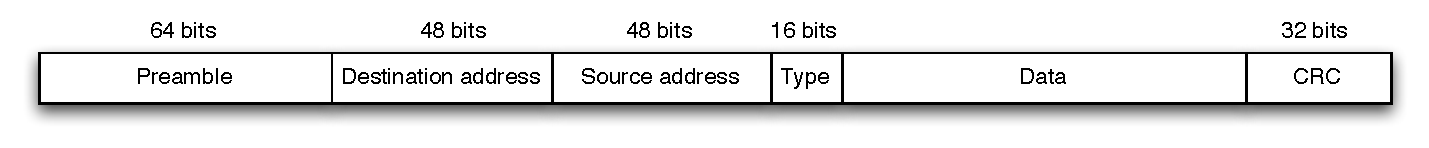
\includegraphics[scale=.75]{graphes/IP/Ethernet}
	\caption{Trame Ethernet}
\end{figure}

\begin{description}
	\item [Préambule] détermine le début d'une trame: “10101010...10101011”;
	\item [Adresse destination] détermine la destination de la trame;
	\item [Type] définit le type de contenu de la trame; à titre d'exemple, si le champ type est à 0800 (en hexadécimal) le champ de données contient un paquet IP. Ainsi, il est possible de déterminer quel protocole de niveau supérieur va utiliser le paquet encapsulé dans le champ de données (Data) de la trame;
	\item [Données] sont les données brutes de la trame à passer au protocole déterminé par le champ \emph{type};
	\item [CRC] est le \emph{checksum} (contrôle de parité) de la trame permettant d'assurer son intégrité.
\end {description}

\chapter{IP: Internet Protocol} % (fold)

\section{Le protocole IP} % (fold)

\subsection{Le datagramme IP} % (fold)

L'en-tête IP est alignée sur des mots de 32 bits. Sa longueur est donc multiple de 4 octets. Par défaut, sans option, l'en-tête IP fait 20 octets de long :

\begin{figure}[h!]
	\center
	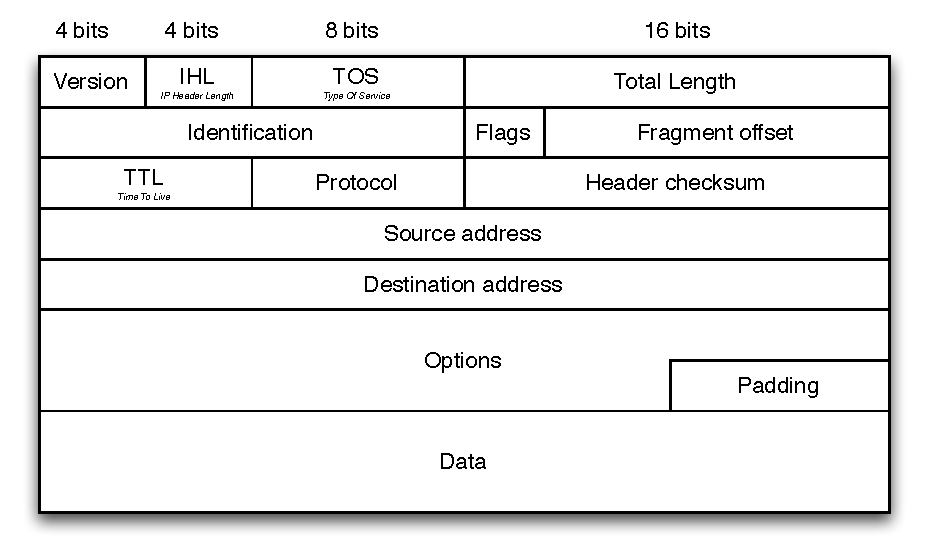
\includegraphics[scale=.75]{graphes/IP/IP}
	\caption{Datagramme IP}
\end{figure}

\begin{description}
	\item [Version] indique le format de l'en-tête. Ce champ sert à l'identification de la version courante du protocole. La version aujourd'hui utilisée porte le n°4;
	\item [IHL \emph{(IP Header Length)}] est la longueur de l'en-tête IP exprimée en mots de 32 bits (5 au minimum, 15 au maximum);
	\item [TOS \emph{(Type Of Service)}] définit le type de service à appliquer au paquet en fonction de certains paramètres comme le délai de transit, la sécurité. Codé sur 8 bits, il comprend les champs suivants:
\end {description}
	\begin{figure}[h!]
		\center
		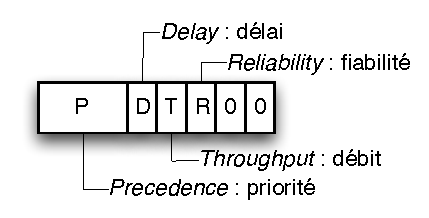
\includegraphics[scale=.75]{graphes/IP/TOS}
		\caption{TOS}
	\end{figure}
\begin{description}
	\item [Total Length] est la longueur totale du datagramme, en-tête et données inclus, exprimée en octets. La longueur d'un datagramme IP est donc limité à 65 535 octets (en pratique il est rare qu'un datagramme IP fasse plus de 1500 octets);
	\item [Identification] est une valeur fournie par l'émetteur aidant au réassemblage des différents fragments du datagramme. Le seul usage de ce champs est donc de permettre à une entité réceptrice de reconnaître les datagrammes qui appartiennent à un même datagramme initial et qui doivent donc faire l'objet d'un réassemblage;
	\item [Flags] est utilisé par la fragmentation. Il est composé de deux indicateurs : \textbf{DF} \emph{(Don't Fragment)} pour interdire la fragmentation et de \textbf{MF} \emph{(More Fragment)} pour signaler des fragments à suivre:
\end {description}
	\begin{figure}[h!]
		\center
		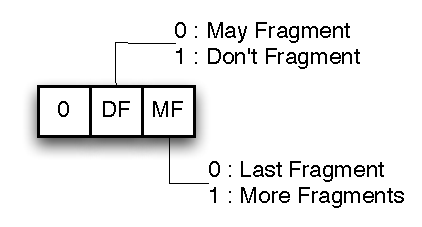
\includegraphics[scale=.75]{graphes/IP/Flags}
		\caption{Flags}
	\end{figure}
\begin{description}
	\item [Fragment Offset] indique sur 13 bits la position relative du fragment dans le datagramme initial, le déplacement étant donné en unités de 64 bits (seuls un datagramme complet ou un premier fragment de datagramme peuvent avoir ce champ à 0);
	\item [TTL \emph{(Time To Live)}] représente une indication de la date limite supérieure du temps de vie d'un datagramme. Cette valeur est comprise entre 0 et 255 et est initialisée par l'émetteur du datagramme, elle est décrémentée tout au long de la route suivie par chaque passerelle traversée. Tout intermédiaire ou destinataire qui détecte le passage de ce champ à la valeur 0 est supposé écarter le datagramme et renvoyer un datagramme ICMP \emph{Time exceeded} à l'émetteur contenant notamment l'en-tête du datagramme détruit. Cette procédure est destinée à éviter les boucles ou les cheminements trop anormaux permettant ainsi de garantir une durée de vie maximale à un datagramme;
	\item [Protocol] indique le protocole (de niveau supérieur) utilisé pour le champ de données du datagramme;
	\item [Header Checksum] est une zone de contrôle d'erreur portant uniquement sur l'en-tête du datagramme;
	\item [Source Adress] est l'adresse IP de la source du datagramme;
	\item [Destination Adress] est l'adresse IP de destination du datagramme;
	\item [Options] sert à des fonctions utiles dans certaines situations (estampillage temporel, sécurité, routage particulier, etc.). Le champ est donc de longueur variable. Il est constitué d'une succession d'options élémentaires, également de longueurs variables. Les options sont codées sur le principe \emph{\textbf{TLV} (Type, Longueur, Valeur)}. La longueur indique la taille complète de l'option en octets. L'option \emph{Record Route} a la structure suivante:
\end {description}
\begin{figure}[h!]
	\center
	\includegraphics[scale=.75]{graphes/IP/"Record Route"}
	\caption{Structure de l'option Record Route}
\end{figure}
\begin{description}
	\item [Padding] permet d'aligner l'en-tête sur 32 bits;
\end {description}

\subsection{Le paquet ARP (\emph{Address Resolution Protocol}) / RARP (\emph{Reverse ARP})} % (fold)

Le protocole ARP permet à une machine d'obtenir l'adresse Ethernet (physique) d'une autre machine, connaissant son adresse IP (logique). Le protocole RARP fait l'inverse. Un paquet ARP (ou RARP) est structuré de la façon suivante:

\begin{figure}[h!]
	\center
	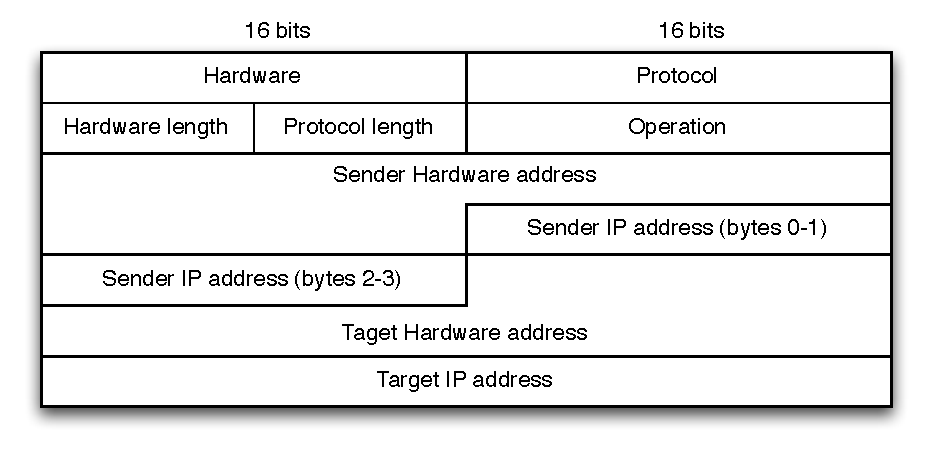
\includegraphics[scale=.75]{graphes/IP/ARP}
	\caption{Paquet ARP}
\end{figure}

\begin{description}
	\item [Hardware] définit le type d'interface pour laquelle l'émetteur cherche une réponse (eg.\lstinline!00 01! pour une interface Ethernet);
	\item [Protocol] définit le type de protocole pour lequel une requête a été émise (eg. \lstinline!08 00! pour une adresse logique IP);
	\item [Hlen] définit la taille de l'adresse physique en octets;
	\item [Plen] définit la taille de l'adresse au niveau protocolaire (IP);
	\item [Operation] décrit le type d'opération à effectuer par le récepteur (eg. \lstinline!00 01! pour une requête ARP (“\lstinline!00 03!” pour une requête RARP), “\lstinline!00 02!” pour une réponse ARP (\lstinline!00 04! pour une réponse RARP));
	\item [Sender HA] définit l'adresse physique (Ethernet) de l'émetteur;
	\item [Sender IA] définit l'adresse de niveau protocolaire (IP) demandé de l'émetteur;
	\item [Target HA] définit l'adresse physique (Ethernet) du récepteur;
	\item [Target IA] définit l'adresse de niveau protocolaire (IP) demandé du récepteur;
\end {description}

\subsection{Le message ICMP (\emph{Internet Control Message Protocol}) } % (fold)

Le protocole ICMP est utilisé lorsqu'un imprévu se produit ou pour tester Internet. Les messages ICMP sont encapsulés dans des datagrammes IP. Ils ont tous en commun le même format pour le premier mot de 32 bits :
\begin{figure}[h!]
	\center
	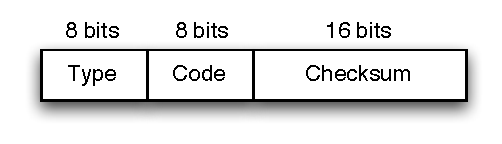
\includegraphics[scale=.75]{graphes/IP/ICMP}
	\caption{ICMP}
\end{figure}

\begin{figure}[h!]
	\center
	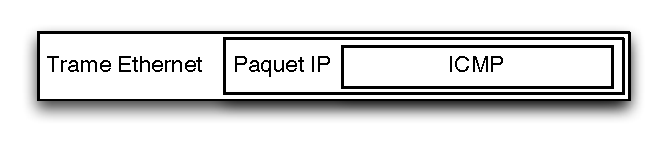
\includegraphics[scale=.75]{graphes/IP/Encapuslation_ICMP}
	\caption{Message ICMP encapsulé dans un datagramme IP}
\end{figure}

A titre d'exemple, \lstinline!Echo! et \lstinline!Echo Reply! sont utilisés pour vérifier l'état d'activité d'une machine. Une machine source envoie alors un message “Echo” à la machine destinataire dont elle veut vérifier l'activité. Celle-ci doit alors lui répondre par un message “Echo Reply”.
\begin{figure}[h!]
	\center
	\includegraphics[scale=.75]{graphes/IP/Echo}
	\caption{Echo}
\end{figure}

\textbf{Principe de l'encapsulation}
\begin{figure}[h!]
	\center
	\includegraphics[scale=.75]{graphes/IP/Encapsulation}
	\caption{Encapsulation}
\end{figure}

\section{Adressage de réseau et routage IP} % (fold)

\subsection{Classes d'adresse} % (fold)

L'espace d'adressage IP est structuré. Une adresse IP est codée sur 4 octets et est constituée de deux parties: une partie \emph{réseau} et une partie \emph{hôte}:

\qquad Adresse IP = \lstinline!<network>.<host>!

Initialement, trois classes d'adresses ont été définie s: \begin{description}
	\item[Classe A] La partie \lstinline!<network>! est codée sur 1 octet (dont le bit de poids fort est égal à \lstinline!0!) et la partie \lstinline!<host>! est codée sur 3 octets;
	\item[Classe B] La partie \lstinline!<network>! est codée sur 2 octets (dont les deux bits de poids fort sont égaux à \lstinline!10!) et la partie \lstinline!<host>! est codée sur 2 octets;
	\item[Classe C] La partie \lstinline!<network>! est codée sur 3 octets (dont les trois bits de poids fort sont égaux à \lstinline!110!) et la partie \lstinline!<host>! est codée sur 1 octet;
\end{description}

Un \emph{\textbf{masque de réseau}} (encore appelé masque “primaire”) est associé à chacune de ces classes:\begin{itemize}
	\item Le masque d'un réseau de classe A est \lstinline!255.0.0.0! (\lstinline!/8!) ;
	\item Le masque d'un réseau de classe B est \lstinline!255.255.0.0! (\lstinline!/16!) ;
	\item Le masque d'un réseau de classe C est \lstinline!255.255.255.0! (\lstinline!/24!).
\end{itemize}

La valeur (optionnelle) spécifiée après le “\lstinline!/!” indique la longueur du préfixe réseau.

En théorie, on dispose de $2^7 = 128$ réseaux de classes A (quelques très grands réseaux), de $2^{14} = 16\,384$ réseaux de classe B (des réseaux intermédiaires) et de $2^{21} = 2\,097\,152$ réseaux de classes C (des petits réseaux).

En pratique, certaines plages d'adresses sont réservées. Par exemple, il n'y a que 126 réseaux de classe A possibles, car un identifiant réseau “tout à 0” signifie “\emph{ce réseau}” et une adresse IP commençant par 127 est une adresse de rebouclage (non routable).

Au maximum, un réseau de classe A peut adresser $2^{24} = 16\,777\,216$ machines, un réseau de classe B peut adresser $2^{16} = 65\,536$ machines et un réseau de classe C peut en adresser $2^8 = 256$. En pratique, les adresses pour lesquelles la partie “hôte” est “tout à 0” ou “tout à 1” sont réservées (au réseau pour la première et au \emph{broadcast} pour la seconde).

\subsection{Sous-réseaux} % (fold)

Tout réseau peut être décomposé en un certain nombre de \emph{\textbf{sous-réseaux}} partageant le même préfixe réseau. L'adresse IP possède alors la forme suivante:

\qquad Adresse IP = \lstinline!<netowork><subnetwork><host>!

Contrairement aux identifiants réseau dont la longueur est prédéterminée par la classe de l'adresse, les préfixes de sous-réseaux peuvent être de longueur variable. La longueur d'un préfixe est choisie selon le nombre de sous-réseaux constituant un site et le nombre d'hôtes par sous-réseaux. Il est donc nécessaire de spécifier pour toute adresse IP affectée, la longueur de son préfixe. C'est la vocation des \emph{\textbf{masques de sous-réseau}}. Le masque associé à une adresse IP est un mot de 32 bits où les seuls bits positionnés à 1 sont ceux associés au préfixe de cette adresse.

Ce procédé rend obsolète la structuration des adresses IP en 3 classes A, B et C. En effet, une adresse réseau appartenant à l'une des 3 classes peut à présent adresser plusieurs réseaux physiques. Les adresses réseaux consécutives et dont la longueur du préfixe le plus long partagé est différente de celle de l'identifiant réseau imposée par sa classe, peuvent être agrégées en une adresse réseau dont la classe spécifierait un identifiant réseau de la longueur de ce préfixe.
\newline

Attribuer des adresses réseau dont la longueur de l'identifiant réseau est variable permet une structuration hiérarchique non plus sur 2 niveaux, mais sur plusieurs niveaux de l'espace d'adressage, indispensable pour résoudre le problème de l'équipement des adresses IP allouables et celui de la taille croissante des tables de routage.

\subsection{Routage IP} % (fold)

Dans un réseau à commutation par paquets, le \emph{\textbf{routage}} est le traitement qui consiste à choisir le chemin sur lequel transmettre un paquet en fonction de son adresse destination et des informations contenues dans les tables de routage. Le \emph{\textbf{protocole de routage}} permet, quant à lui, de construire dynamiquement les tables de routage. Une \emph{\textbf{table de routage}} (ou FIB, \emph{Forwarding Information Base}) est une structure complexe qui contient les informations nécessaires pour atteindre toute adresse IP valide.

Un Internet est composé de plusieurs réseaux interconnectés par des équipements appelés \emph{\textbf{gateways}} (\emph{\textbf{passerelles}} ou \emph{\textbf{routeurs}}). Chaque \emph{gateway} est directement connecté à au moins deux réseaux physiques et assure le transfert des paquets (relaye les paquets) d'un réseau à un autre. Un \emph{\textbf{hôte}} est directement connecté à au moins un réseau physique mais ne relaye jamais de paquet. Ainsi, contrairement au \emph{gateways}, il rejette systématiquement les paquets qu'il reçoit et dont il n'est pas le destinataire. En théorie, un hôte n'exécute donc pas de protocole de routage et ses tables de routage sont généralement construites manuellement par l'administrateur réseau.

Il existe deux façons de faire du routage dans IP:\begin{description}
	\item[Le routage direct] Concerne la transmission d'un paquet IP entre deux machines connectées au même réseau physique (pas de \emph{gateway} impliquée). La source encapsule le paquet dans une trame dont l'adresse de destination est l'adresse MAC (Ethernet) de la destination ;
	\item[Le routage indirect] Intervient lorsque la destination n'est pas connectée au même réseau physique que la source. La transmission du paquet est alors effectuée de proche en proche (\emph{hop by hop}); le routage IP fournit l'adresse du prochain routeur sur le chemin vers la destination souhaitée (\emph{gateway} la plus proche de la destination). Chaque paquet est alors encapsulé dans une trame dont l'adresse MAC de destination est celle de la \emph{gateway} empruntée.
\end{description}
	
Une table de routage IP est constituée d'au moins quatre colonnes :

\begin{tabularx}{\linewidth}{|X|X|X|X|}
  \toprule
  Destination & Mask & Gateway & Interface \\
  \midrule
  	{\footnotesize Destination que permet de joindre cette entrée. Il peut s'agir d'une adresse complète d'hôte ou d'une adresse réseau; {\ttfamily 0.0.0.0} correspond à la route par défaut.}  
	& {\footnotesize Spécifie, si la destination s un (sous-)réseau, le masque de ce (sous-)réseau. Si la destination est un hôte, elle contient {\ttfamily 255.255.255.255}. Si l'entrée est celle de la route par défaut, elle contient {\ttfamily 0.0.0.0}.}
	& {\footnotesize Indique l'adresse du prochain routeur. Si l'adresse de destination est celle d'un hôte ou d'un réseau directement accessible par une interface locale, apparaît, selon les systèmes, {\ttfamily 0.0.0.0} ou un astérisque.}
	& {\footnotesize Indique l'interface (la carte Ethernet) sur laquelle le paquet doit être transmis pour suivre la route considérée.} \\
  \bottomrule
\end{tabularx}

L'algorithme, simplifié, suivant permet à un routeur de déterminer, lorsqu'il reçoit un paquet IP contenant l'adresse IP “DestAdr”, sur quelle interface il doit le relayer. Les entrées de la table de routage sont notées :\begin{itemize}
	\item \lstinline!(H, 255.255.255.255, G, I)! si l'adresse \lstinline!H! est celle d'un hôte ;
	\item \lstinline!(R, M, G, I)! si l'adresse \lstinline!R! est celle d'un réseau.
\end{itemize}

\begin{algorithm}[H]
	\DontPrintSemicolon
	\Deb{
		\Si{$\exists$ entrée \lstinline!(H, 255.255.255.255, G, I)! telle que \lstinline!DestAdr = H!}{
			 Routage comme spécifié dans la table (direct si \lstinline!G = *!, indirect sinon) sur l'interface \lstinline!I!.
		}\Sinon{
			\Si{$\exists$ entrée \lstinline!(R, M, G, I)! telle que \lstinline!(DestAdr AND M) = R!}{
				 Routage comme spécifié dans la table (direct si \lstinline!G = *!, indirect sinon) sur l'interface \lstinline!I!
			}\Sinon{
				\Si{$\exists$ route par défaut \lstinline!(0.0.0.0, 0.0.0.0, G, I)!}{
					Routage indirect via \lstinline!G! sur l'interface \lstinline!I!
				}\Sinon{
					Envoyer une erreur \emph{host unreachable} ou \emph{unreachable network} à l'application émettrice
				}
			}
		}
	}
	\caption{Algorithme de routage}
\end{algorithm}

Il est à noter que si plusieurs entrées de la table de routage conviennent (\emph{match}), l'algorithme choisit celle dont l'adresse possède le plus de bits identiques avec celle du paquet (\emph{best matching}).

\textbf{Exemple de routage}
\begin{figure}[h!]
	\center
	\includegraphics[scale=.65]{graphes/IP/Routage}
	\caption{Routage d'un paquet d'un utilisateur X vers un serveur Y}
\end{figure}

\section{Fragmentation} % (fold)

Un message utilisateur de 2048 octets de données et de 20 octets d'en-tête est envoyé d'un hôte A vers un hôte B en empruntant un seul routeur. Le premier sous-réseau traversé utilise un en-tête de trame de 14 octets et une MTU (\emph{Maximum Transfer Unit}) de 1024 octets, alors que le second sous-réseau utilise un en-tête de trame de 8 octets et une MTU de 512 octets.

On considérera que:
\begin{itemize}
	\item La MTU inclut les en-têtes de trame et les en-têtes IP ;
	\item Le champ “Fragment Offset” est codé sur 13 bits; il exprime, en unités de 8 octets, la position relative des données contenues dans le fragment par rapport au datagramme initial ;
	\item Aucune option IP n'est utilisée ;
	\item Les sous-réseaux n'introduisent pas de déséquencement.
\end{itemize}

\chapter{UDP et TCP: Protocoles de transport} % (fold)

\section{UDP (\emph{User Datagram Protocol})} % (fold)

\subsection{Format de message} % (fold)

\begin{figure}[h!]
	\center
	\includegraphics[scale=.75]{graphes/TCP/paquet_UDP}
	\caption{Paquet UDP}
\end{figure}

\subsection{Fonctionnalités assurées par UDP} % (fold)

UDP est le protocole de transport (i.e de bout en bout) le plus simple qui soit. Il se contente d'étendre le service de remise de machine à machine (offert par IP) en un service de communication de processus à processus.

A ce titre, il assure essentiellement une fonction de \emph{\textbf{(dé)multiplexage}} grâce aux champs \lstinline!Source Port! et \lstinline!Destination Port!, qui permettent d'identifier (quoique de façon indirecte) les processus de communication sur les deux machines distantes. On notera que c'est la paire (port, hôte) appelée \emph{socket}, qui constitue la clé de démultiplexage pour UDP.

S'il n'y a pas de contrôle d'erreur à proprement parler, il y a néanmoins une fonction de \textbf{détection d'erreur} (optionnelle pour IPv4 mais obligatoire pour IPv6) qui repose sur le champ \lstinline!Checksum!: elle permet de vérifier que le message UDP a bien été délivré entre les deux bons ports (l'adresse IP \lstinline!dest! aurait pu être modifiée lors du transit su paquet, ce qui aurait provoqué une remise à un mauvais destinataire). Lorsqu'il est calculé, le \emph{checksum} porte sur la totalité du message UDP augmentée d'un pseudo-header comportant entre autre les @ IP source et destination (en conséquence de quoi UDP repose forcément sur IP).

En théorie les messages UDP peuvent être fragmentés par IP. En pratique, la plupart des applications utilisant UDP limitent la taille de leurs messages à 512 octets, pour éviter toute fragmentation.

\section{TCP (\emph{Transmission Control Protocol})} % (fold) 

\subsection{Généralités} % (fold)

TCP est u protocole de transport, donc de bout en bout, offrant un service de remise \textbf{fiable} de flux d'octets en \textbf{full-duplex} et en \textbf{mode connecté}. Il met notamment en œuvre des mécanismes de:
\begin{itemize}
	\item (Dé)multiplexage;
	\item Contrôle d'erreur;
	\item Contrôle de flux;
	\item Contrôle de congestion.
\end{itemize}

À la différence des protocoles en mode connecté que nous avons pu voir jusqu'à présent, TCP n'utilise qu'un seul format de segment qui sert aussi bien à établir/libérer une connexion qu'à transférer des données:
\begin{figure}[h!]
	\center
	\includegraphics[scale=.75]{graphes/TCP/paquet_TCP}
	\caption{Paquet TCP}
\end{figure}

\begin{description}
	\item [Source Port et Source Destination] Identifient les extrémités locales de la connexion. Les numéros jusqu'à 1024 correspondent à des ports réservés (eg. le port 21 correspond à FTP, le port 80 à HTTP);
	\item [Sequence Number] est le numéro de séquence du premier octet de données du segment TCP, si le drapeau \textsc{syn} est à 1, ce numéro est l'ISN (\emph{Initial Sequence Number}) et le premier octet de données sera numéroté ISN + 1;
	\item [Acknowledgment Number] est le numéro d'acquittement, si le drapeau \textsc{ack} est à 1, ce numéro contient la valeur du prochain numéro de séquence que l'émetteur est prêt à recevoir;
	\item [Data Offset] est la longueur de l'en-tête TCP exprimée en mots de 32 bits; elle indique donc où les données commencent ;
	\item [Reserved] n'est pas utilisé et doit être mis à zéro;
	\item [URG] drapeau positionné à 1 si le pointeur d'urgence est en cours d'utilisation;
	\item [ACK] drapeau positionné à 1 pour indiquer la validité du numéro d'acquittement;
	\item [PSH] drapeau positionné à 1 pour indiquer au destinataire de remettre les données à l'application concernée dés leur arrivée;
	\item [RST] drapeau positionné à 1 pour réinitialiser une connexion devenue incohérente, pour rejeter un segment altéré ou pour rejeter une tentative d'ouverture de connexion;
	\item [SYN] drapeau positionné à 1 lors d'une phase d'établissement de connexion;
	\item [FIN] drapeau positionné à 1 lors d'une phase de libération de connexion ;
	\item [Window] fenêtre d'anticipation de taille variable; la valeur de ce champ indique au récepteur combien il peut émettre d'octets après l'octet acquitté;
	\item [Checksum] champs de contrôle portant sur tout le segment augmenté d'un pseudo en-tête, constitué principalement des adresses IP source et destination;
	\item [Urgent Pointer] pointeur indiquant l'emplacement des données urgentes; utilisé uniquement si le flag \lstinline!urg! est positionné à 1;
	\item [Options] champs de longueur variable offrant des possibilités non offertes dans l'en-tête de base (eg. Détermination du MSS (\emph{Maximum Segment Size}), la taille maximum d'un segment TCP (en fait la taille maximum du champs de données d'un segment TCP, car MSS n'inclue pas l'en-tête));
	\item [Padding] champs permettant de cadrer l'en-tête TCP sur des mots de 32 bits;
\end {description}

\subsection{Établissement de connexion} % (fold)

L'établissement d'une connexion TCP se fait par échange de trois messages (\emph{three-way handshake}):
\begin{figure}[h!]
	\center
	\includegraphics[scale=.75]{graphes/TCP/Etablissement}
	\caption{Etablissement de connexion}
\end{figure}
\begin{rem*}
	Avec 2 messages, le sous-réseau pouvant déséquencer les paquets, l'appelant de la connexion reçoit un segment de données pour une connexion qui est en attente de confirmation d'établissement.

Avec 3 messages, l'appelé doit attendre de recevoir un acquittement de sa confirmation (sous la forme de données ou d'acquittement) avant de pouvoir émettre ses propres données. On évite ainsi à l'appelant de se retrouver dans un état mal défini.
\end{rem*}

Une connexion TCP est identifiée par (port S, hôte S, port D, hôte D). Il est tout à fait possible d'ouvrir une connexion entre les machines A et B, ports X et Y, de la fermer, puis quelque temps après, d'ouvrir une nouvelle connexion, toujours entre les machines A et B et es ports X et Y. On parle dans ce cas d'\emph{\textbf{incarnations}} différentes d'une même connexion. Le scénario suivant est alors possible:
\begin{figure}[h!]
	\center
	\includegraphics[scale=.75]{graphes/TCP/Numero_sequence}
	\caption{Problème de numérotation}
\end{figure}

On y voit une seconde incarnation réutilisant un numéro de séquence trop tôt, c'est-à-dire quand il y a encore une chance qu'un segment appartenant à une incarnation précédente interfère avec l'incarnation courante.

Le numéro de séquence initial (ISN -- \emph{Initial Sequence Number}) est choisi de façon à éviter cette situation. À l'origine, il devait être tiré aléatoirement; en pratique, il est généralement mis à jour grâce à un compteur de 32 bits incrémenté toutes les 4 µs.
\newline

\begin{rem*} Lorsqu'un hôte A reçoit deux segments SYM en provenance d'un même port hôte B, le second SYN peut être une retransmission du SYN original ou alors une nouvelle requête de connexion (cas de panne suivie d'un redémarrage de B). Si le SYN est une retransmission, alors sa valeur de ISN est la même que dans le premier SYN. Dans le cas contraire, et si les valeurs d'ISN sont générées par une horloge, alors l'ISN du second SYN sera différent de celui du premier SYN.
\end{rem*}

\subsection{Numérotation des données} % (fold)

L'une des principales propriétés de TCP est la fiabilité. TCP doit résoudre les problèmes de données en erreur, perdues, dupliquées ou délivrées dans le mauvais ordre par le système de communication Internet. Cela est réalisé au moyen d'un numéro de séquence assigné à chaque octet transmis, et d'un numéro d'acquittement (ACK) envoyé par le récepteur TCP. Si l'ACK n'est pas reçu pendant une durée de temporisation fixée (\emph{Timeout}), la donnée doit être retransmise. Au niveau du récepteur, les numéros de séquence sont utilisées pour ordonner correctement les segments qui ont pu être reçus dans u ordre incorrect, et pour éliminer les duplications. Les erreurs sont détectées par un champ de contrôle présent dans chaque segment TCP transmis, et vérifié par le récepteur. Si ce champ a une valeur incorrect, le segment TCP est ignoré.

TCP numérote donc ses octets de données et non pas ses segments. Le numéro de séquence du premier octet de données est transmis avec le segment, dans le champ \lstinline!SequenceNumber! de l'en-tête TCP (32 bits), et est appelé numéro de séquence du segment.

\subsection{Acquittement des données} % (fold)

Les segments TCP véhiculent également un numéro d'acquittement (\lstinline!AckNum!) dans le champ \emph{Acknowledgment Number}, qui représente le numéro de séquence du prochain octet de données attendu dans le flux de données en sens inverse. Un segment TCP est “acceptable” si son \lstinline!AckNum! est compris dans la plage:
\[
           \textrm{Plus “grand” \texttt{SeqNum} envoyé et non encore acquitté} < \texttt{AckNum} \le \textrm{Prochain \texttt{SeqNum} à envoyer}
\]
Un segment non acceptable est rejeté et provoque l'envoi d'un acquittement portant les numéros \lstinline!SeqNum! et \lstinline!AckNum! courants.

\begin{figure}[h!]
	\center
	\includegraphics[scale=.75]{graphes/TCP/Acquittement}
	\caption{Acquittement}
\end{figure}

\subsection{Contrôle de flux} % (fold)

Pour son contrôle de flux, TCP utilise un mécanisme de fenêtre coulissante de taille variable.

TCP offre un moyen pour le récepteur de contrôler la quantité de données envoyées par l'émetteur. Cela est réalisé en retournant avec chaque acquittement, une “fenêtre” indiquant la plage des numéros de séquence acceptables à partir du dernier segment correctement reçu. Cette fenêtre indique les numéros des octets que l'émetteur a le droit de transmettre avant de recevoir plus d'autorisations du récepteur.

La taille courante de la fenêtre est communiquée dans le champ \lstinline!Window! du segment.

TCP est orienté octet: la numérotation et la fenêtre portent sur des octets. TCP décide de constituer et d'envoyer un segment lorsque:\begin{enumerate}
	\item Dès qu'il y a MSS (\emph{Maximum Segment Size}) octets de données à envoyer MSS = MTU du sous-réseau local -- en-tête IP -- en-tête TCP (les entités TCP se communiquent leur MSS respectifs au moment de l'établissement (champ options) et c'est la valeur la plus faible qui l'emporte. Par défaut la MSS est de 536 octets (+ 20 en-tête));
	\item Lorsque son application lui demande explicitement: TCP supporte une fonction \lstinline!push! que le processus peut invoquer pour vider le \emph{buffer} des octets en attente d'émission;
	\item Sur expiration d'un temporisateur: pour éviter d'attendre trop longtemps les MSS octets.
\end{enumerate}

\subsection{Temporisateur de retransmission} % (fold)

Un élément important du contrôle d'erreur est le temporisateur de retransmission.\\
Il faut mesurer le temps écoulé entre l'envoi d'un octet de données ayant un numéro de séquence donné et la réception de l'acquittement couvrant ce numéro de séquence. Cette mesure s'appelle \textbf{RTT} (\emph{Round Trip Time}). Il faut alors calculer le SRTT (\emph{Smoothed Round Trip Time}) de la façon suivante:
\[
           SRTT = \alpha \times SRTT + (1 - \alpha)\times RTT
\]
et en déduire le temporisateur de retransmission, RTO (\emph{Retransmission TimeOut}):
\[
           RTP = \min\left[UBOUND, \max\left[LBOUND, (\beta \times SRTT)\right]\right]
\]
où $UBOUND$ et $LBOUND$ sont les bornes supérieure et inférieure sur les \emph{timeout}, $\alpha$ est un facteur de pondération et $\beta$ est un facteur lié à la variance du délai.

\subsection{Libération de connexion} % (fold)

\begin{figure}[h!]
	\center
	\includegraphics[scale=.75]{graphes/TCP/Liberation}
	\caption{Libération de connexion}
\end{figure}
   
\chapter{Web et HTTP} % (fold)
\label{cha:web_et_http}

Réseau d'extrémité : \begin{itemize}
	\item Système d'extrémité (ie. machines hôtes) : se situent à la périphérie du réseau et exécutent des programmes applicatifs (eg. email, web\dots) ;
	\item Modèle client/serveur : ;
	\item Modèle pair-à-pair : pas (ou peu) de serveurs (eg. Sykype, BitTorrent, KaZaA\dots).
\end{itemize}

\begin{figure}[h!]
	\center
	\includegraphics[scale=.75]{graphes/relations-protocoles}
	\caption{Relations entre les protocoles}
\end{figure}

\begin{figure}[h!]
	\center
	\includegraphics[scale=.75]{graphes/demux-protocoles}
	\caption{Démultiplexage des protocoles}
\end{figure}

Architecture des applications

\begin{description}
	\item [Client serveur] Des machines clientes demandent et reçoivent un service depuis un serveur \emph{always-on} (eg. navigation/serveur Web).\begin{itemize}
		\item Serveur :\begin{itemize}
			\item S'exécute toujours sur un équipement terminal ;
			\item Configuré avec une adresse IP permanente ;
			\item Ferme de serveurs pour passer le facteur d'échelle.
		\end{itemize}
		\item Client : \begin{itemize}
			\item Communique avec un serveur ;
			\item Eventuellement connecté par intermittence ;
			\item Configuré avec une adresse IP qui peut être dynamique ;
			\item Ne communique pas directement avec d'autres pairs.
		\end{itemize}
	\end{itemize}
	\item[Pair-à-Pair] Pas (ou peu) de serveurs (eg. Sykype, BitTorrent, KaZaA\dots).\begin{itemize}
		\item Un pair n'est pas toujours un serveur ;
		\item Communication directe entre équipements terminaux arbitraires ;
		\item Les pairs changent d'adresse IP et sont connectés par intermittence.
	\end{itemize}
\end{description}

Communication entre processus

Un processus est un programme qui s'exécute sur une machine hôte. 

Sur une même machine hôte, deux processus communiquent entre eux en utilisant un mécanisme de communication \textbf{inter-processus} (tubes, segment de mémoire partagée, signaux\dots) défini au niveau su système d'exploitation.

Les processus s'exécutant sur des machines hôtes différentes communiquent en échangeant des \textbf{messages}.\begin{itemize}
	\item Processus client : initie la communication ;
	\item Processus serveur : processus qui boucle, en attente d'être contacté par un processus client.
\end{itemize}
\begin{rem*}
	Les applications P2P sont constituées de processus à la fois client \textbf{et} serveur.
\end{rem*}

\begin{tabularx}{\linewidth}{lXX}
	\toprule
	& TCP & UDP\\
	\midrule
	Description & Orienté connexion : mis en place d'une connexion entre les processus clients et serveur (à l'initiative du client) permettant un transport \textbf{fiable} entre les processus émetteur et récepteur. & Transfert de données en mode non connecté non fiable entre processus émetteur et récepteur.\\
	Contrôle de flux & Eviter qu'un émetteur n'engorge un récepteur & Pas fourni\\
	Contrôle de congestion & Régulation du débit d'émission de l'émetteur en fonction de la saturation du réseau & Pas fourni\\
	Garanties & Pas de garanties temporelles ou de bande passante minimum & Respect de contraintes temporelles, bande passante garantie\\
	\bottomrule
\end{tabularx}

Applications usuelles

\begin{tabularx}{\linewidth}{XXXXXX}
	\toprule
	Application & Perte de données & Bande passante & Garantie temporelle & Protocole & Protocole de transport\\
	\midrule
	Transfert de fichiers & Pas de perte & Elastique & Aucune & FTP (RFC 959) & TCP\\
	Email & Pas de perte & Elastique & Aucune & SMTP (RFC 2821) & TCP\\
	Web & Pas de perte & Elastique & Aucune & HTTP (RFC 2616) & TCP\\
	Streaming & Tolérant & Audio : 5kbps-1Mbps ; vidéo : 10kbps-5Mbps & Propriétaire (eg. RealNetworks) & TCP/UDP\\
	Téléphonie IP & Tolérant & Audio : 5kbps-1Mbps & Propriétaire (eg. Vonage, DialPad) & UDP\\
	\bottomrule 
\end{tabularx}

\begin{def*}[Socket]
	Un socket est une interface locale, créée à l'initiative d'une application, contrôlée par le système d'exploitation à travers laquelle les processus applicatifs peuvent envoyer et recevoir des messages à/depuis un autre processus applicatif. 
	
	Un socket est donc un point d'accès offert aux applications pour accéder aux protocoles de transport de bout-en-bout (TCP/UDP).
\end{def*}

Interface de programmation Socket introduite dans BSD4.1 UNIX en 1981. Elle est utilisable par des applications pour créer, utiliser et libérer des sockets. C'est un paradigme client/serveur. Deux types de services de transport sont accessibles via l'API Socket : \begin{itemize}
	\item Non fiable, datagramme ;
	\item Fiable, orienté flux d'octets.
\end{itemize}

\begin{figure}[h!]
	\center
	\includegraphics[scale=.75]{graphes/socket}
	\caption{Démultiplexage des protocoles}
\end{figure}

\section{HTTP (HyperText Transfer Protocol)}

HTTP est un protocole de la couche application (couche 7). Il implémente deux programmes : un programme client et un programme serveur. Ces programmes s'exécutent sur deux machines distantes et s'échangent des messages HTTP.

HTTP définit le format des messages, et comment le client et le serveur se les échangent.

Une page web est constituée d'objets. Un objet peut être un fichier HTML, une image JPEG, un applet Java, un fichier audio\dots Ces objets sont adressables par une URL. La page web est constituée d'un document (fichier) de base qui contient des objets référencés.

HTTP utilise TCP de la manière suivante : \begin{itemize}
	\item Le client initie une connexion TCP (création d'un socket) vers le serveur HTTP sur le port de destination 80 ;
	\item Le serveur accepte la connexion TCP émanent du client ;
	\item Des messages HTTP (du protocole de niveau 7) sont échangés entre le navigateur (client HTTP) et le serveur Web (serveur HTTP) ;
	\item Fermeture de la connexion TCP .
\end{itemize}

HTTP est un protocole \emph{sans état} : le serveur ne maintient aucune information concernant les requêtes du client. 

Echanges HTTP :\begin{description}
	\item[Non persistant] Au plus un objet est envoyé ans une connexion TCP. Utilisé par HTTP/1.0.\begin{itemize}
		\item Requière 2 RTT par objet référencé (document de base inclus) ;
		\item Surcharge de l'OS pour chaque connexion TCP ;
		\item Les navigateurs ouvrent souvent des connexions TCP concurrentes (ie. en parallèle) pour récupérer les objets référencés.
	\end{itemize}
	\item[Persistant] Plusieurs objets peuvent être envoyés sur une même connexion TCP entre le client et le serveur. Utilisé par HTTP/1.1 par défaut. \begin{itemize}
		\item Le serveur laisse la connexion ouverte après l'envoi de la réponse ;
		\item Les messages HTTP suivants entre le client et le serveur sont envoyés sur la même connexion ;
		\item Fermeture de la connexion TCP sur un \emph{timeout}.
		\item Il existe deux types de connexions persistantes : \begin{itemize}
			\item \textbf{Sans pipelining} : un client émet une nouvelle requête seulement si la réponse précédente à été reçus. Un RTT pour chaque objet référencé ;
			\item \textbf{Avec pipelining} : un client envoie une nouvelle requête dès qu'il détecte la présence d'un objet référencé (ie. lors du \emph{parsing} du document de base). Par défaut dans HTTP/1.1.
		\end{itemize}
	\end{itemize}
\end{description}

Types de méthodes :\begin{itemize}
	\item Méthode POST : s'applique à la page Web qui propose un formulaire. Les valeurs saisies sont renvoyées au serveur dans le champ \emph{entity body}.
	\item Méthode GET : les valeurs saisies sont renvoyées dans le champ \emph{url} sous la forme \lstinline!?key=value&key_1=value_1!.
	\item Méthode HEAD : demande au serveur de laisser les objets demandés hors de la réponse ;
	\item Méthode PUT (HTTP/1.1) : permet d'uploader un fichier placé dans le champ \emph{entity body} à l'adresse spécifiée dans le champ \emph{url}.
	\item Méthode DELETE : supprime sur le serveur le fichier spécifié dans le champ \emph{url}.
\end{itemize}

Codes de statut HTTP

\begin{tabularx}{\linewidth}{lX}
	\toprule
	Code & Description\\
	\midrule
	200 & \lstinline!OK!\newline Requête accédée, l'objet demandé se trouve plus bas dans le message.\\
	301 & \lstinline!Moved permanently!\newline L'objet demandé a été déplacé , son nouvel emplacement est spécifié plus bas dans le message.\\
	400 & \lstinline!Bad Request!\newline La requête n'a pas été comprise par le serveur.\\
	404 & \lstinline!Not Found!\newline Le document demandé n'a pas été trouvé sur le serveur.\\
	505 & \lstinline!HTTP Version Not Supported!\newline Problème de compatibilité des versions HTTP\\
	\bottomrule 
\end{tabularx}

% chapter web_et_http (end)

\chapter{Annexes} % (fold)

\section{Equipements} % (fold)

	\begin{tabularx}{\linewidth}{>{\setlength\hsize{0.4\hsize}}X>{\setlength\hsize{0.3\hsize}}X>{\setlength\hsize{2.3\hsize}}X}
\hline 
Equipement & Couche OSI & Rôle\tabularnewline
\hline
\hline 
Amplificateur (\emph{amplifier}) & 1 & Amplification d'un signal analogique.\tabularnewline
\hline 
Répéteur (\emph{Repeater}) & 1 & Régénération du signal, dans le cadre d'une transmission numérique
(signal numérique ou analogique représentant des données numériques).\tabularnewline
\hline 
Hub & 1 & Répéteur multiports : répète les informations provenant d'un port
vers tous les autres ports raccordables. Il ne limite pas les collisions
et n'améliore pas l'utilisation de la bande passante.\tabularnewline
\hline 
Pont (\emph{Bridge}) & 2 & Relie plusieurs segments d'un réseau local. Filtre les trames en ne
laissant passer sur un segment donné que celles qui sont destinées
à des équipements situés sur ce segment. Un pont ne génère pas de
collisions : il attend le moment propice pour émettre (il peut stocker
les trames). 

\begin{minipage}{0.7\textwidth}
\medskip Fonctionnement :\par
\begin{itemize}
\item apprentissage : le pont construit lui-même sa table d'adresses MAC, au fur et à mesure qu'il reçoit des trames.
\item algorithme de \emph{Spanning Tree} : pour éviter les boucles.
\item mode \emph{promiscuous} : mode bloquant dès que l'on émet une trame.
\end{itemize}
\medskip
\end{minipage}
\tabularnewline
\hline 
Commutateur (\emph{switch}) & 2 & Un commutateur de niveau 2 fonctionne selon le même principe qu'un pont, mais il est plus performant grâce à sa matrice de commutation plus rapide.\tabularnewline
\cline{2-3} 
 & 3 & Utilisé par exemple dans les réseaux X25. Lors de l'établissement du circuit virtuel, il prend des décisions de routage et il garde un état de chaque connexion pour ensuite aiguiller les paquets en fonction de leur numéro de voie logique. Un commutateur de niveau 3 fonctionne dans un environnement homogène, à la différence d'un routeur.\tabularnewline
\hline 
Routeur (\emph{Router}) & 3 & Prend des décisions de destination ; un routeur possède au moins deux interfaces réseau. Un routeur permet de relier des sous-réseaux différents.\tabularnewline
\hline 
Passerelle (\emph{gateway}) & variable & Terme générique qui permet de désigner des équipements travaillant à différents niveaux : passerelle de niveau 1, 2, 3, etc.\tabularnewline
\hline
\end{tabularx}

\begin{sidewaystable}
\begin{tabularx}{\textwidth}{>{\bfseries}lXX} 
	\toprule
	 	& Mode CV & Mode datagramme\\[0.05in]\bottomrule
	Adressage 	& Chaque paquet contient une identification de CV & Tous les paquets doivent contenir adresse source et adresse destination $\Rightarrow$ overhead\\[0.05in]
	Routage 	& Tous les paquets suivent la même route $\Rightarrow$ tables de routage + tables de commutation & Chaque paquet est routé indépendamment des autres \\[0.05in]
	Contrôle de congestion & Facile (réservation de ressources) & Difficile \\
	\bottomrule
\end{tabularx}
\caption{Commutation Mode CV vs. Mode datagramme}
\end{sidewaystable}

\begin{sidewaystable}
\begin{tabularx}{\textwidth}{>{\bfseries}lXXX} 
	\toprule
	Acheminement		& Principe & Avantages & Inconvénients\\[0.05in]\bottomrule
	Voie logique 			& \begin{itemize}
	\item mode connecté
	\item les paquets suivent la même route : aucun déséquencement
	\item décision de routage à l'établissement de la connexion ; même route pour tous les paquets
	\item possibilité de préallouer les ressources dans chque n\oe ud traversé par la connexion
	\item possibilité d'utiliser une fenêtre de contrôle de flux sur chaque connexion
	\end{itemize} & \begin{itemize}
		\item étiquette de petite taille
	\end{itemize} & \begin{itemize}
	\item vulnérabilité, sensibilité aux pannes d'un n\oe ud u d'une liaison
	\item gestion de la table de translation et place mémoire nécessaire pour la table
	\end{itemize} \\[0.05in]
		
	Datagramme 	& \begin{itemize}
	\item mode non connecté
	\item aucune route n'est établie à l'avance ; décision de routage est prise pour chaque paquet
	\item déséquencement des paquets (routage individuel)
	\item il suffit que la source connaisse l'adresse du destinataire pour pouvoir émettre
	\end{itemize} & \begin{itemize}
		\item flexibilité $\Rightarrow$ robustesse face aux défaillances + réactivité face au phénomène de congestion
		\item répartition du trafic (paquets routés indépendamment)
	\end{itemize} & \begin{itemize}
		\item temps de commutation dans les n\oe uds plus important (décision de routage)
	\end{itemize}\\
	\bottomrule
\end{tabularx}
\caption{Routage Mode d'acheminement par voie logique vs. par datagramme}
\end{sidewaystable}

\begin{sidewaystable}
\begin{tabularx}{\textwidth}{>{\bfseries}llXX} 
	\toprule
	 						& Algorithme & Avantages & Inconvénients\\[0.05in]\bottomrule
	Etat des liens 			& Bellman-Ford & \begin{itemize}
	\item plus stable : chaque routeur est censé connaître la topologie du réseau
	\item permet $\neq$ métriques : chaque LSP pet transporter plusieurs coût
	\item converge plus vite
	\end{itemize} & Aucun \\[0.05in]
		
	Vecteurs de distance 	& Dijkstra & \begin{itemize}
		\item overhead réduit : pas de précaution pour empêcher la corruption des données
		\item moins d'espace mémoire nécessaire
	\end{itemize} & Aucun non plus\\[0.05in]
	\bottomrule
\end{tabularx}
\caption{Routage à états des liens vs. routage à vecteurs de distance}
\end{sidewaystable}

\begin{sidewaystable}
\begin{tabularx}{\textwidth}{>{\bfseries}lXX} 
	\toprule
	 						& Avantages & Inconvénients\\[0.05in]\bottomrule
	Bus 	& \begin{itemize}
	\item facile à installer
	\item retrait implicite des informations (terminateur)
	\item topologie passive : la panne d'une machine n'a pas d'incidence sur le réseau $\Rightarrow$ robustesse
	\end{itemize} & \begin{itemize}
		\item Risques de collision $\Rightarrow$ temps d'accès indéterministe
		\item unités d'accès passives $\Rightarrow$ signal non régénéré (besoin de répéteurs)
		\item non adapté à la fibre optique (support unidirectionnel)
		\item rupture du support $\Rightarrow$ réseau HS (rebonds du signal aux 2 nouvelles extrémités)
	\end{itemize} \\[0.05in]
		
	Etoile 	& \begin{itemize}
		\item Conflits d'accès générés en central
		\item technologie simple et éprouvée
		\item panne d'une machine $\Rightarrow$ déconnexion de la branche de la machine en cause
		\item fibre optique utilisable (liaison point à point)
	\end{itemize} & \begin{itemize}
		\item problèmes de fiabilité du point central
		\item taille du réseau dépend de la puissance du point central
		\item plus le réseau est grand, plus il faut de câblage
	\end{itemize}\\[0.05in]
	
	Anneau 	& \begin{itemize}
		\item pas de taille limite au réseau
		\item fibre optique (liaison point à point)
		\item temps de transfert borné
	\end{itemize} & \begin{itemize}
		\item Retrait des informations nécessaires
		\item problème de fiabilité si l'anneau se coupe ($\Rightarrow$ doubler l'anneau)
		\item connecteurs complexes et coûteux
		\item topologie active : panne d'une machine $\Rightarrow$  panne du réseau
	\end{itemize}\\[0.05in]
	\bottomrule
\end{tabularx}
\caption{Topologies}
\end{sidewaystable}

\end{document}
